\pagebreak
\chapter{Power BI}
\setcounter{section}{0}

\section{Working with M (Power Query) in Power BI}
\begin{description}
\item[Funktion] Eine \textbf{Funktion} ist ein mathematische Objekte, welches eine spezielle Relation, angewandt auf eine definierte Menge, ist. Dabei wir jedem Input genau ein Output zugewiesen. Um genau zusein, ist die Funktion die Abbildungsregel, das Objekte lautet Abbildung. Mann nennt Abbildungen auch Funktionen, wenn sie ein ein Tupel aus Reelen Zahlen abbildet (Check). Beispiel: $f:\R \rightarrow \R$
\item[Expression] Eine \textbf{Expression} ist ein \textbf{algebrasiche} oder \textbf{syntakische Phrase}. In Power Query spricht man von Expression und meint damit ganze Zeilen Ausdrücke. 
\item[Value] Es gibt verschiedene Datenstrukturen. Dabei können diese auch aus mehreren zusammengebaut sein. 
\end{description}

Die Datentypen in Power Query sind ähnlich zu anderen Programmierungssprachen. Es gibt jedoch Ausnahmen. Ist kein Wert für eine Zelle vorhanden, so wird Type \textbf{Null}. Weiter Datetypen werden im Folgenden beschreiben. Hierbei werden spezielle Funktionen verwandt, um diesen Wert zu erzeugen. Dabei werden bestimmt Syntaxen verlangt.\\

\subsection{Variable}
Variablen werden bei erzeugen in $M$ nicht deklariert. Eine automatische Zuweisung der Typen funktioniert über die Syntax. Für Funktionen können jedoch Typen für Inputvariablen und die Funktion selbst definiert werden.
\begin{figure}[H]
	\centering
	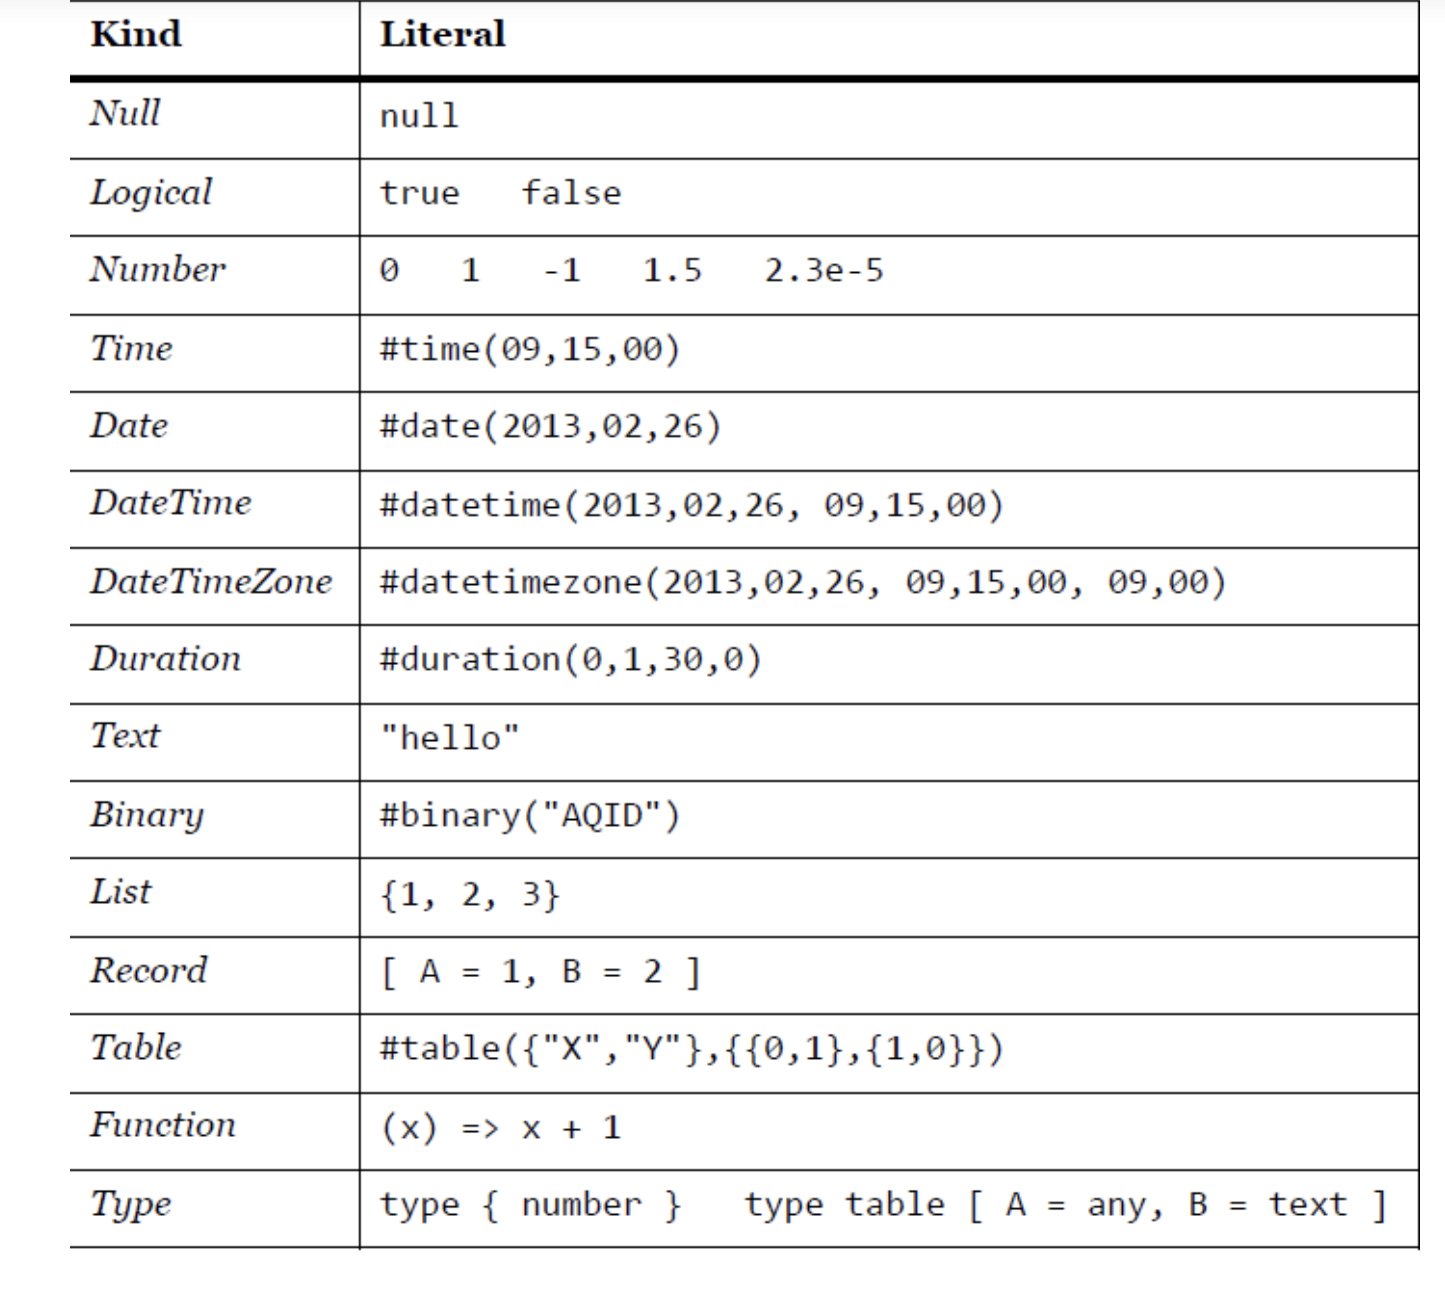
\includegraphics[scale = 0.3]{attachment/chapter_1/screenshot030}
	\caption{}
	\label{fig:screenshot030}
\end{figure}
\href{https://radacad.com/basics-of-m-power-query-formula-language}{Link}

\subsubsection{Variable name}
Variablen werden in Power Query, wie auch in anderen Sprachen, mit Hilfe einer Zeichenkette definiert. Es gibt jedoch die Besonderheit, das Variablennamen auch mit einem Leerzeichen definiert werden dürfen. Dafür muss der Name als String gesehen werden und mit einem $\#$ am Anfang versehen werden.
\begin{lstlisting}[style=M]
let
	#"Das ist wirklich ein Variablenname!" = 13,
	y = #"Das ist wirklich ein Variablenname!"
in
	y // Returns 13
\end{lstlisting} 

\subsubsection{Zuweisen / Syntax}
Für das Zuweisen eines Types zu einer Variablen wird der \textbf{as} Ausdruck verwandt. Wird eine Variable erzeugt ohne eine Funktion zu verwenden, erfolgt eine automatische Type-Zuweisung.
\begin{lstlisting}[style=M]
let 
	y = 1.3234 // type number
	#"Variable 2" = "Text" // type text
	#"Variable 3" = #date(1,1,1908) // Zuweisung erfolgt durch die intrinsische Funtkion date
\end{lstlisting}
Der \textbf{as} Ausdruck wird verwandt, um Input und Output von Funktionen zu definieren. 
 \begin{lstlisting}[style=M]
let
	Funktion1 = (Input as number) as number => 2 + 3
in
	Funktion1
\end{lstlisting}
Wollen wir einen Typen einer Spalte einer Tabelle ändern, so nutzen wir die

\begin{figure}[H]
	\centering
	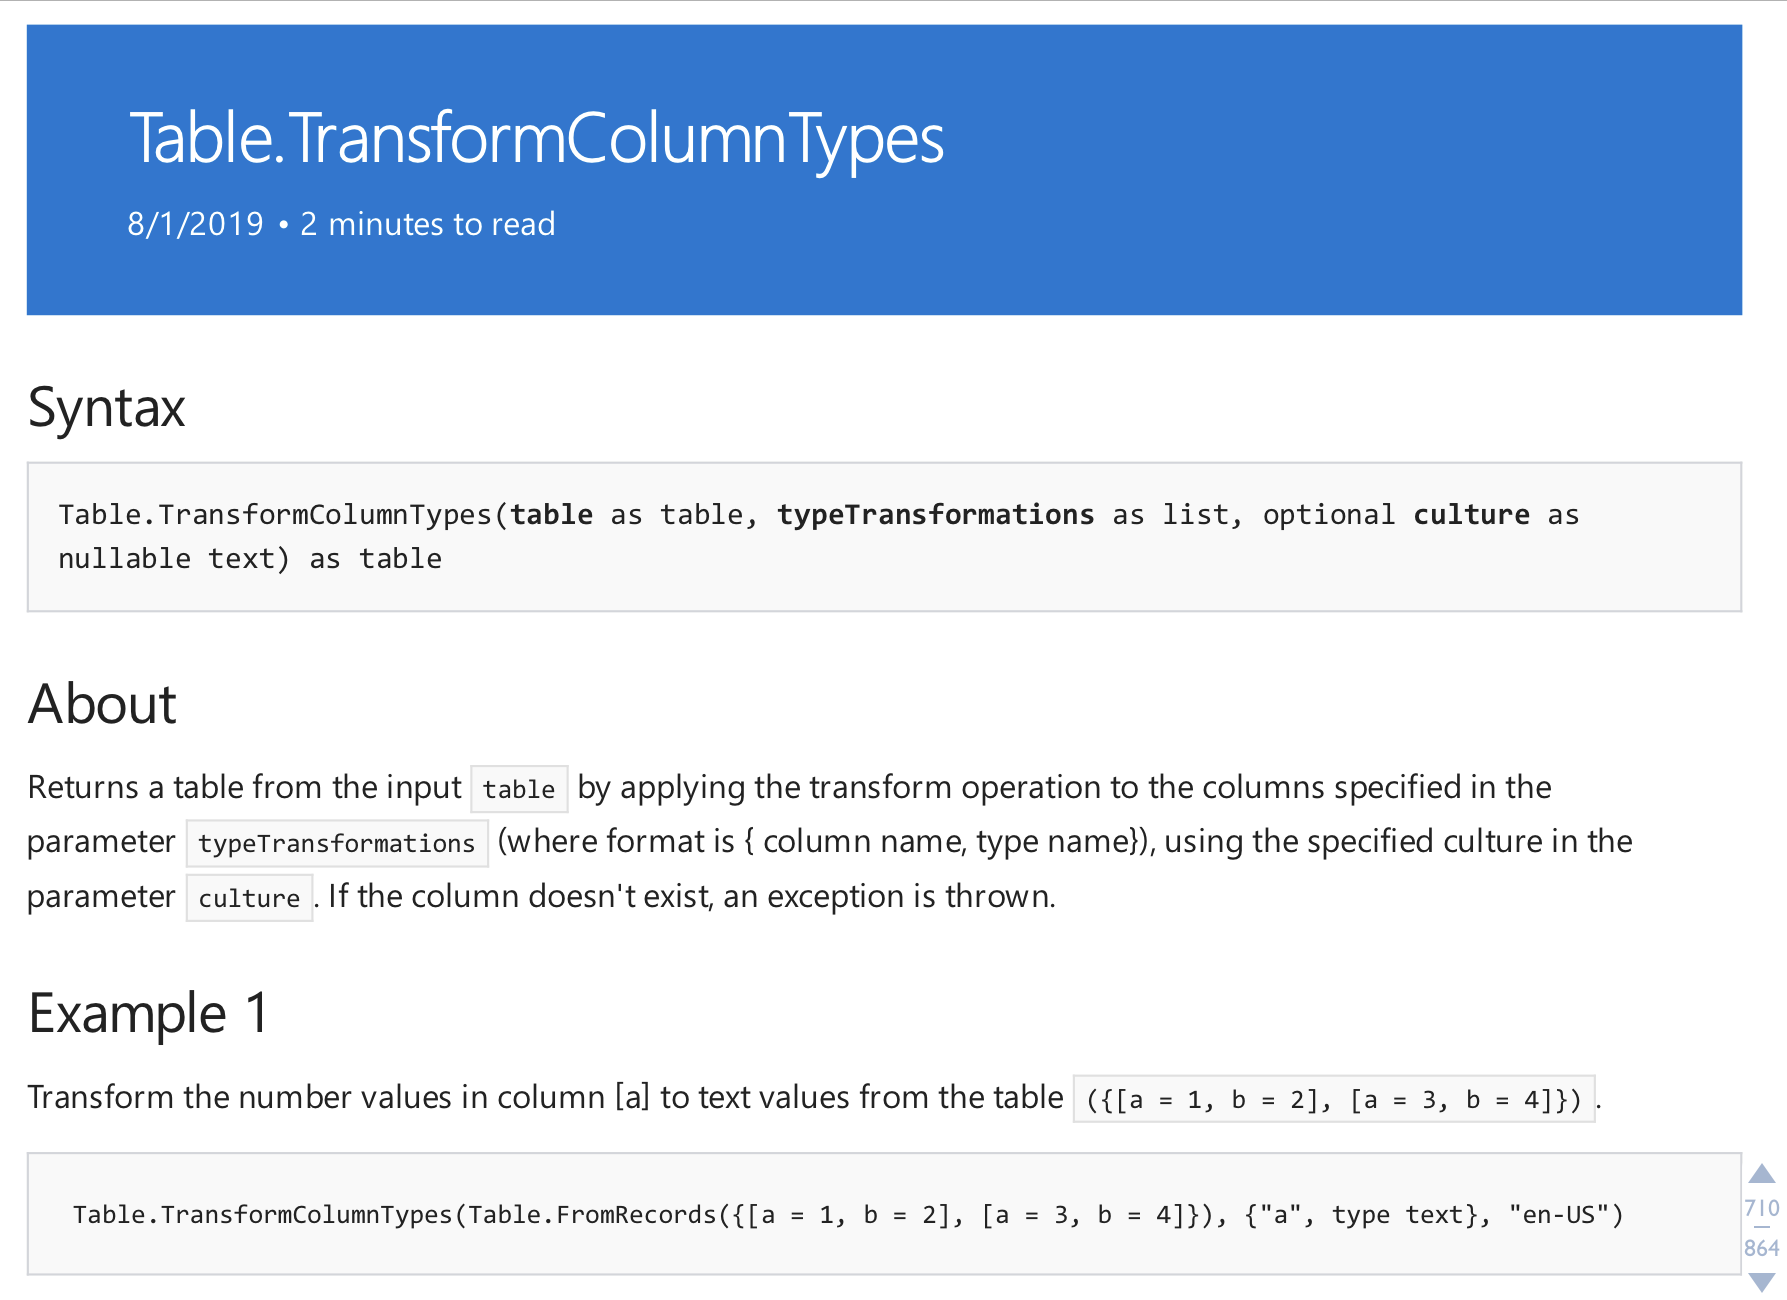
\includegraphics[scale = 0.3]{attachment/chapter_1/screenshot033}
	\caption{}
	\label{fig:screenshot033}
\end{figure}
Die Funktion ließt eine Tabelle als Input ein. Für die Transformation wir eine \textit{Liste} benötigt. Diese benötigt jedoch für jeden Eintrag selber eine Liste, mit dem ersten Eintrag den Spaltennamen und den zweiten den zu bezeichneten Typ.
Beispiel:
\begin{figure}[H]
	\centering
	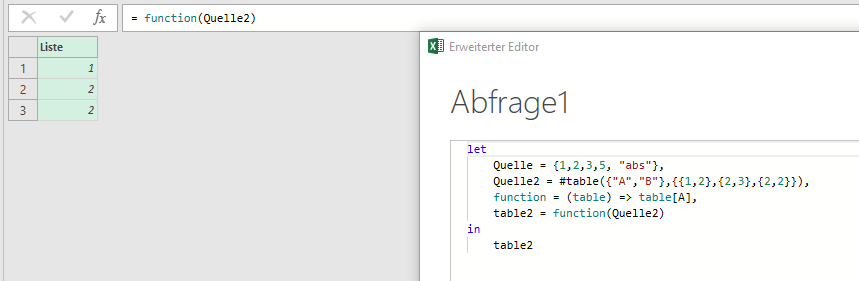
\includegraphics[scale = 0.3]{attachment/chapter_1/screenshot032}
	\caption{Eine Spalte}
	\label{fig:screenshot032}
\end{figure}

\begin{figure}[H]
	\centering
	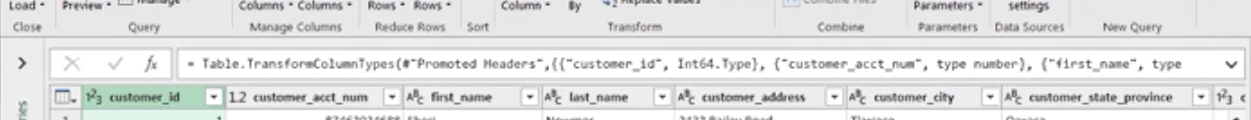
\includegraphics[scale = 0.3]{attachment/chapter_1/screenshot034}
	\caption{Mehrere Spalten}
	\label{fig:screenshot034}
\end{figure}

\textbf{Achtung} Es können verschiednen Syntaxen verwendet werden um eine Typ zu definieren. 
\begin{figure}[H]
	\centering
	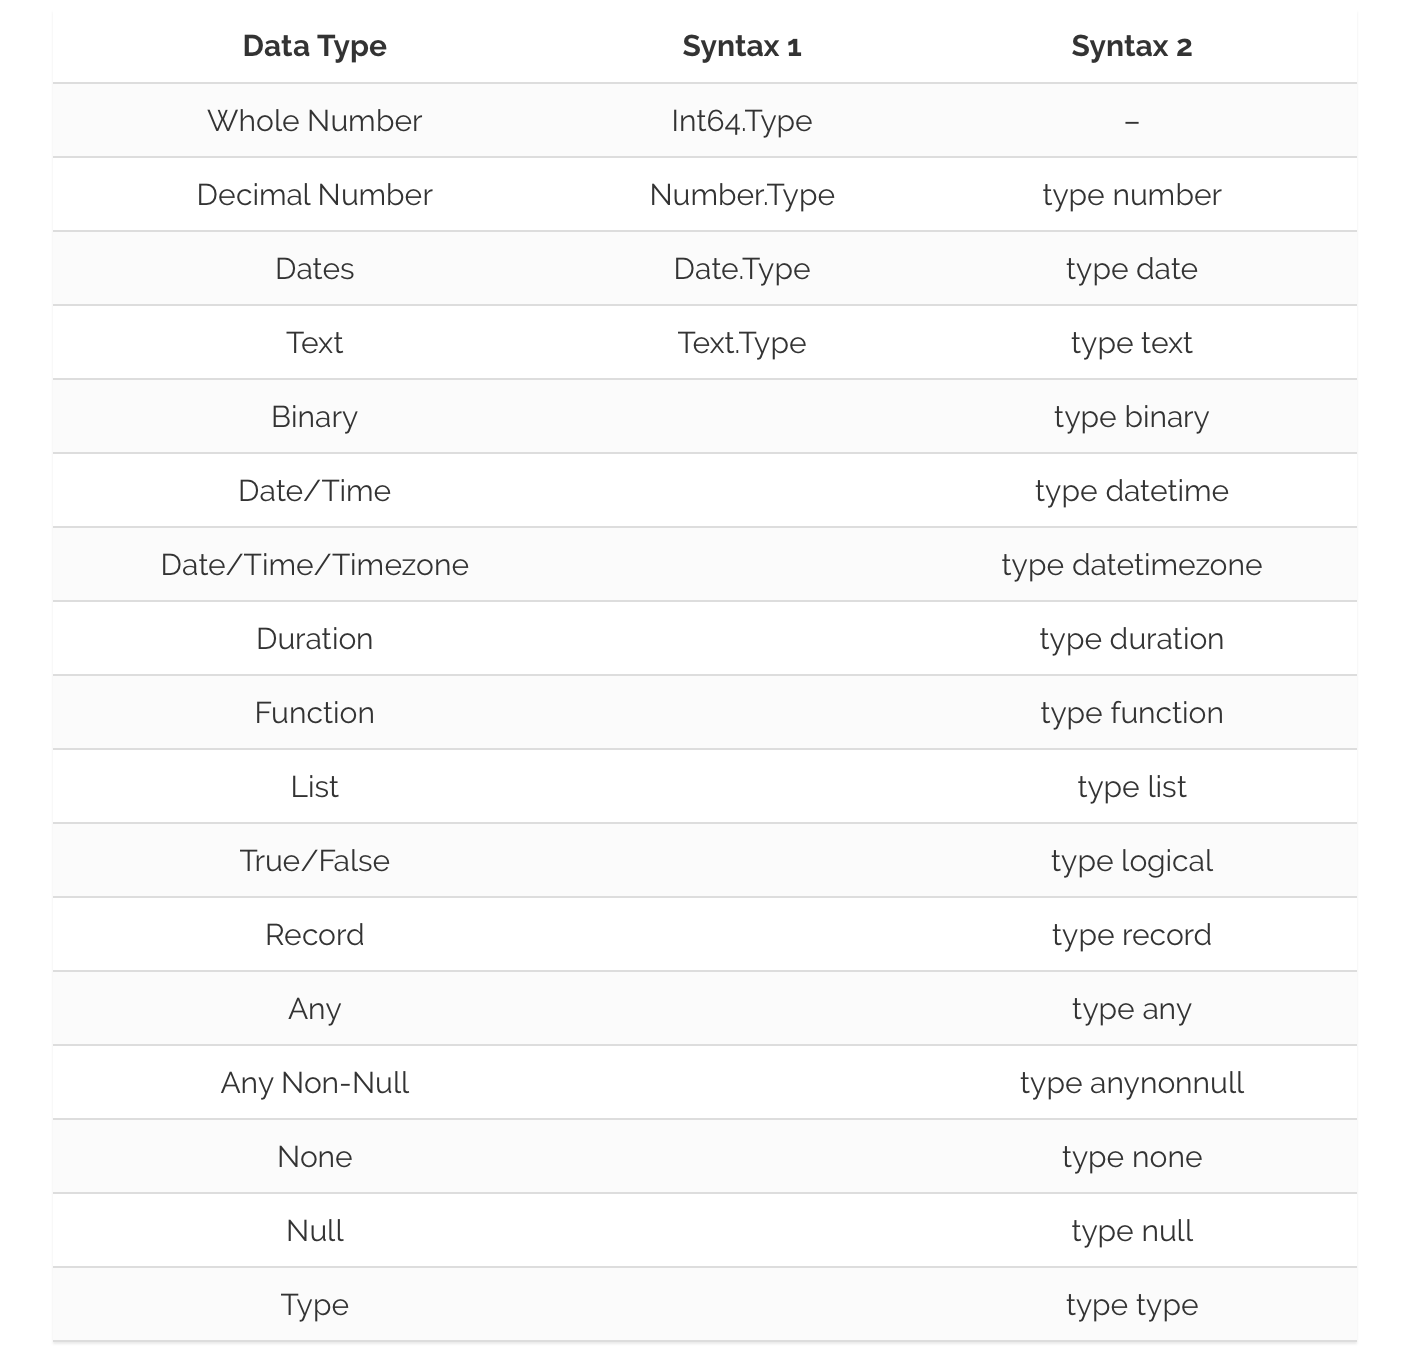
\includegraphics[scale = 0.3]{attachment/chapter_1/screenshot035}
	\caption{Mehrere Spalten}
	\label{fig:screenshot035}
\end{figure}
Dies sieht man auch im Beispiel mit mehren Spalten. Die Integer Typumwandlung erfolgt mit dem $"$Int64.Type$"$ dieser wird jedoch nicht $"$type Int64$"$ geschrieben. Für andere Typen kann diese Logik aber angewandt werden.

\subsubsection{number, text, logical}
Variablen müssen 
\begin{lstlisting}[style=M]
let
	x = 5,
	y = x + 5, 
	w = "Test Text",
	z = true,
in 
	x // Returns 
\end{lstlisting}

\subsubsection{null}
Variablen besitzen eine Ausprägung für einen Wert. Das Konzept von $"$any$"$ and $"$null$"$ wird hier nicht berücksichtigt. Diese typen können ebenfalls abgerufen werden. Dabei kann eine Funktion eine Input auf den \textit{type type} testen. 


\begin{lstlisting}[style=M]
let
	y = null // y ist vom Typ null
	w = "null" // w ist vom Typ text
	z = 0 // z ist vom Typ number
in 
	w // Return null
\end{lstlisting}

\subsubsection{Type}
Der Type \textbf{type} wird wie intrinsische Varialben mit eine Prefix deklariert. Der Prefix lautet $"$type$"$ und der Variablentype wird in $\left\lbrace \, \right\rbrace$. Für Tabellen können die Typen für die Spalten gleich mit im Tabellenkopf vermerkt werden.
\begin{lstlisting}[style=M]
let 
	x = type {number}, // Die Variable x ist vom type type.
	y = #table(
			{Column1, Cloumn2}, // Kopf der Tabelle ohne Typen
			{
				{2, "text"},
				{4, "hello"}
			}
		),

	w = #table(
			type table [Column1 = type number, Column2 = type text], 
			\\ Kopf der Tabelle mit Typen 
			{
				{2, "text"},
				{4, "hello"}
			}
		)

in
	y 
\end{lstlisting} 
\subsubsection{Intrinsiche Werte}
Um Werte wie \textit{date, duration, binary} etc. zu schaffen, werden spezielle \textbf{single intrinsic function} benötigt. Man erkennt diese daran, dass vor ihnen ein $\#$ steht. 

\begin{lstlisting}[style=M]
let
	x = #date(2019,2,2)
in
	x // Returns 2019-2-2
\end{lstlisting} 

\subsection{Strukturierte Variablen} 
Es gibt drei verschiedene Datentypen, welche aus mehreren Komponenten bestehen

erden.
\href{https://www.howtoexcel.org/power-query/m-code/}{Link}, \href{https://docs.microsoft.com/en-us/powerquery-m/expressions-values-and-let-expression}{Link}

\begin{lstlisting}[style=M]
let
	x = {a,2,abc} // List
	y = [ // Record
			variable1 = 1,
			Item = "abc,
			ID = 4
		], 
	w = #table(
			{"Column1", "Column 2" },
			{
				{2, 4},
				{"abs", 5},
				{123j,#date(2019,2,2)}
			}
in
	x{3} // Returns abc
	// y[Item] returns abs
	// w{2}[Column1] returns 123j; 2 ist die zweite Zeile (Start 0) 
\end{lstlisting} 

\subsubsection{List} Eine Liste ist ein einfaches Array, welches alle verschiedene Typen von Objekten beinhalten kann. 
\subsubsection{Record} Ein Record ist ein Array, welches zu jedem Eintrag eine Indexnamen ausweisen kann. Es können auch Records von Records gemacht werden.
\subsubsection{Table} Eine Tabelle teilt sich in den Tabellenkopf und die Zeilen auf. Um eine Table zu erstellen, muss die intrinsische Funktion $\#table()$ angewandt werden.\\

Bei der Erstellung der Tabellen, können gleich \textbf{typen} von Datenformaten gewählt werden, siehe Zuweisen/ Syntax. 

\subsubsection{Beispiele}
\begin{lstlisting}[style=M]
let  
    Source =   
{  
   1,   
   "Bob",   
   DateTime.ToText(DateTime.LocalNow(), "yyyy-MM-dd"),   
   [OrderID = 1, CustomerID = 1, Item = "Fishing rod", Price = 100.0]   
}  
in   
    Source 
\end{lstlisting}
Das Result ist: 

\begin{figure}[H]
	\centering
	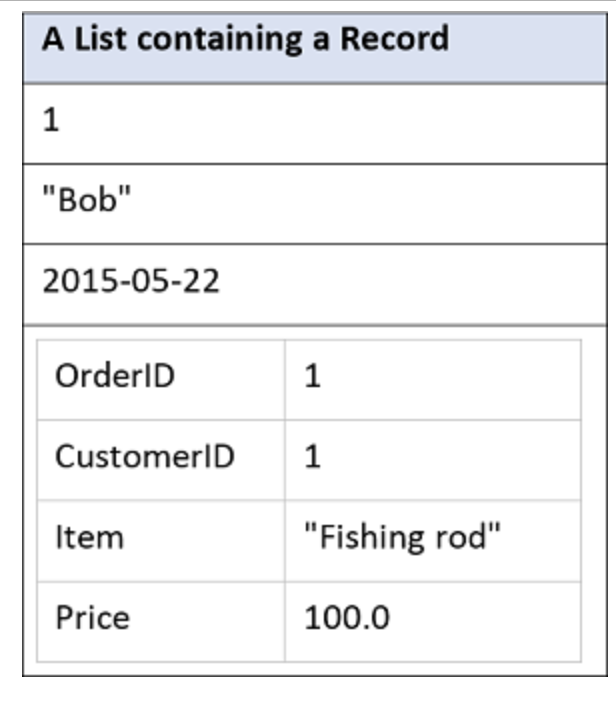
\includegraphics[scale = 0.3]{attachment/chapter_1/screenshot031}
	\caption{}
	\label{fig:screenshot031}
\end{figure}


\subsection{Function} 
Eigenen Funktionen können ebenfalls geschrieben werden. Es ist jedoch die sequenzielle Natur des M-Codes zu berücksichtigen. Eine Besonderheit zur Sprache $C++$ ist, dass die Typen für Input und Output Variablen nicht dekliniert werden müssen. Es wird dann von \textbf{impliziten Funktionen} gesprochen. Der \textit{Tye any} wird dann als \textit{Default} genutzt:
\subsubsection{Implicite function}
\begin{align}
\text{Name der Funktion } = \left(\text{ Inputvariablen }\right) = > \text{Expression}, 
\end{align} 
\begin{lstlisting}[style=M]
let  
	Add = (x, y) => x + y,
	AddResualts = 
		[
			OnePlusTwo = Add(1,2) // Ergebnis ist 3
			OnePlusOne = Add(1,1) // Ergebnis ist 2
		]
in   
   AddResualts 
   /*
   OnePlusTwo 3
   OnePlusOne 2
   */
\end{lstlisting}

\subsubsection{Explicite function}
Bei dieser Art von Funktionen müsse die Typen für die Input- wie Outputvariablen angegeben werden. Dies erfolgt im zweiten Block. 
\begin{align}
\text{Name der Funktion } = \left(\text{ Inputvariablen as $"$type$"$ }\right) \text{as $"$type$"$} = > \text{Expression}, 
\end{align} 
Mit etwas geschickt, können auch komplexere Funktionen gebaut werden.

\begin{lstlisting}[style=M]
let
	GreaterThenFive = (list) =>
		let
			OrderedList = List.Select(list, each _ >= 5) 
			/*
			List.Select(list as list, selection as function) as list
			*/
			Result = List.First(OrderedList)
		in 
	Record = [
		Ergebnis1 = GreaterThenFive({1,2,6}) // Returns 6
		Ergebnis2 = GreaterThenFive({12,12,45,23}) // Returns 12
		]
in 
	Record
\end{lstlisting} 
\subsubsection{Bewertungen (Conditions)}
Es ist essentielle für das Verstehen der meisten Funktionen, wie Tabllen, Listen, Records abgerufen und Teilmengen der Informationen selektiert werden können.
\begin{description}
\item[Table]
\begin{figure}[H]
	\centering
	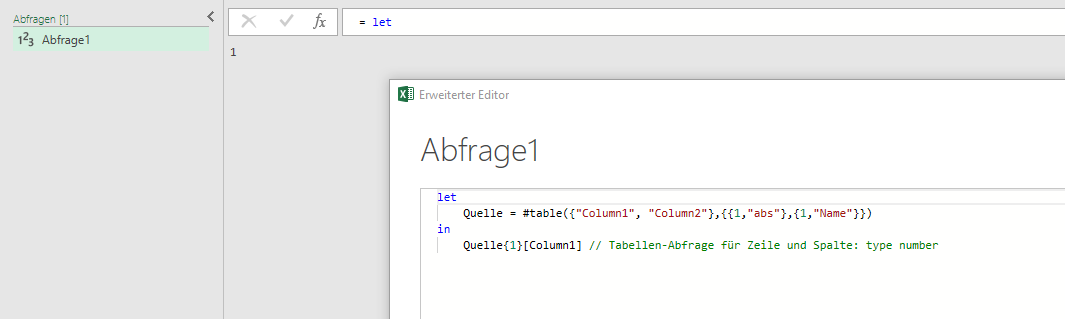
\includegraphics[scale = 0.3]{attachment/chapter_1/screenshot052}
	\caption{Tabelle - Zeile und Spalte (type cell-type}
	\label{fig:screenshot052}
\end{figure}
\begin{figure}[H]
	\centering
	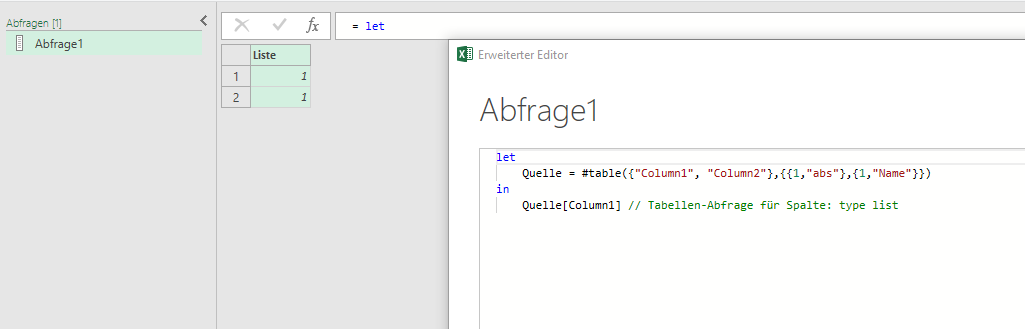
\includegraphics[scale = 0.3]{attachment/chapter_1/screenshot053}
	\caption{Tabelle - Spalte (type list)}
	\label{fig:screenshot053}
\end{figure}
\begin{figure}[H]
	\centering
	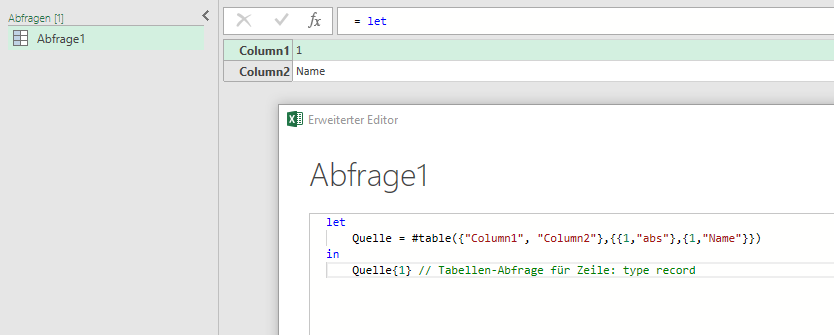
\includegraphics[scale = 0.3]{attachment/chapter_1/screenshot054}
	\caption{Tabelle - Zeile (type record}
	\label{fig:screenshot054}
\end{figure}
\item[Record]
\begin{figure}[H]
	\centering
	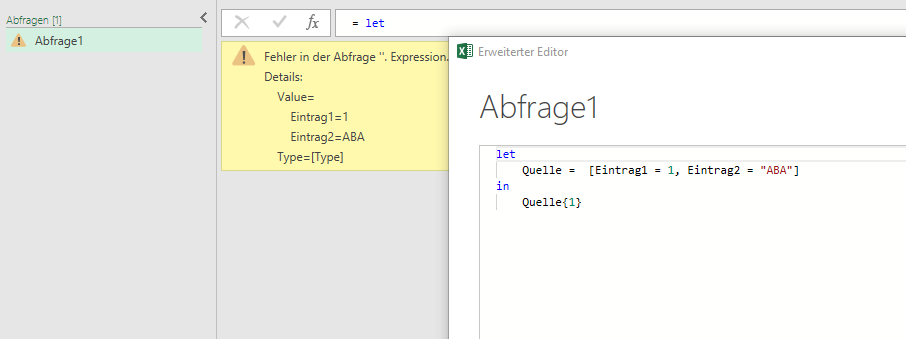
\includegraphics[scale = 0.3]{attachment/chapter_1/screenshot055}
	\caption{Record - Zeile ${}$: Geht nicht!)}
	\label{fig:screenshot055}
\end{figure}
\begin{figure}[H]
	\centering
	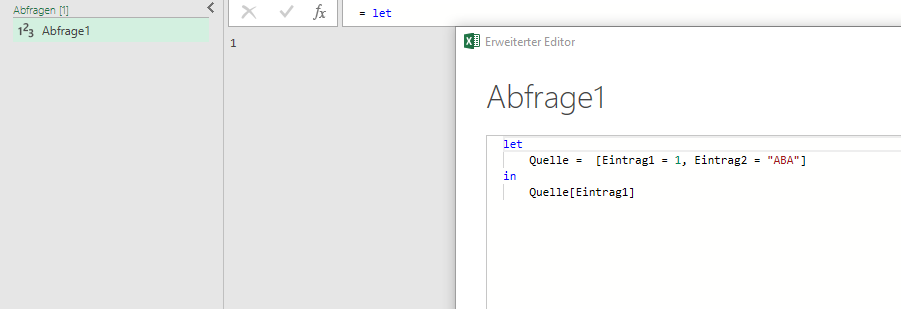
\includegraphics[scale = 0.3]{attachment/chapter_1/screenshot056}
	\caption{Record - Eintrag [] (type cell-type}; Wichtig: Table.SelectRows()
	\label{fig:screenshot056}
\end{figure}
\item[List]
\begin{figure}[H]
	\centering
	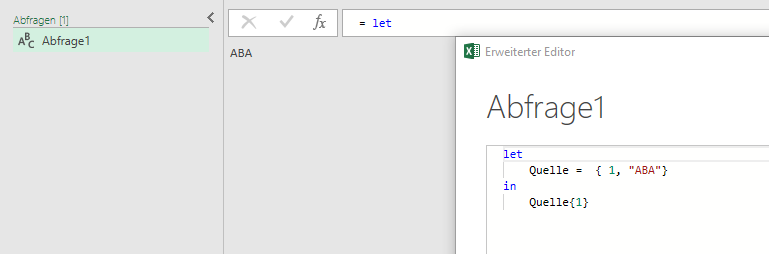
\includegraphics[scale = 0.3]{attachment/chapter_1/screenshot044}
	\caption{Liste - Zeile (type cell-type}
	\label{fig:screenshot0}
\end{figure}
\end{description}
Eine Funktion kann als Outputwert vom \textit{type logic} sein, sie kann aber auch jeden anderen Wert annehmen. Wichtig ist jedoch, wird eine Logische Abfrage im Funktionskörper veranlasst und diese nicht verarbeitet, so nimmt die Funktion den Typen logic an.\\

Eine Funktion kann, wenn ihr eine Tabelle übergeben wird, eine Liste wieder geben, wenn aus der Tabelle eine Spalte mit $[]$ ausgelesen wird, siehe \ref{fig:screenshot032}. Wird die ausgelesene Liste verglichen mit einem einzelnen Wert, so wird die logische Abfrage \textit{false} wiedergeben, da die beiden typen nicht gleich sind.

\begin{figure}[H]
	\centering
	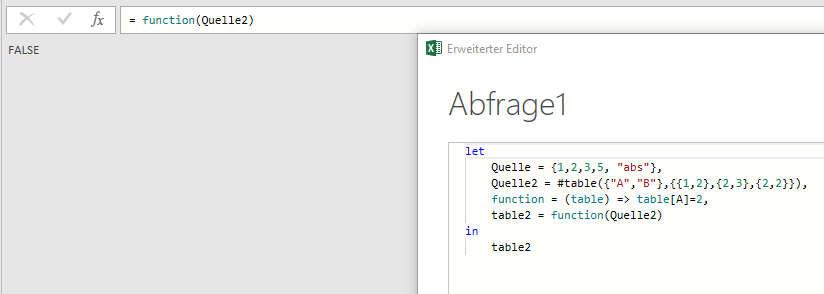
\includegraphics[scale = 0.3]{attachment/chapter_1/screenshot043}
	\caption{}
	\label{fig:screenshot043}
\end{figure}
Selbst wenn jeder Eintrag in der List den gleichen zuüberprüfenden Eintrag hat, gibt die Funktion \textit{false} wieder

\begin{figure}[H]
	\centering
	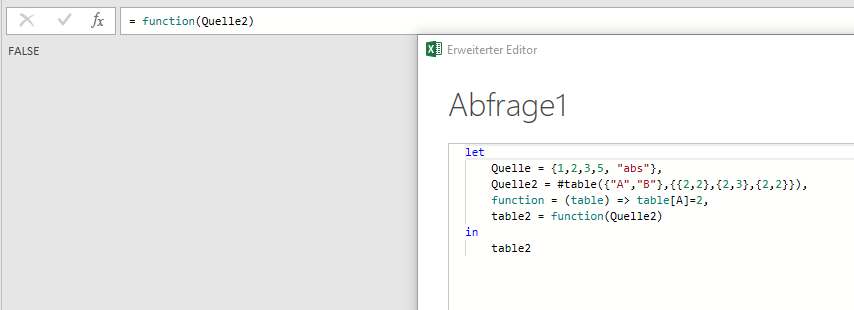
\includegraphics[scale = 0.3]{attachment/chapter_1/screenshot036}
	\caption{}
	\label{fig:screenshot036}
\end{figure}
Wird ein Abgleich mit einer List gemacht, welche die gleichen Einträge beinhaltet, so gibt die Funktion \textit{true} wieder.

\begin{figure}[H]
	\centering
	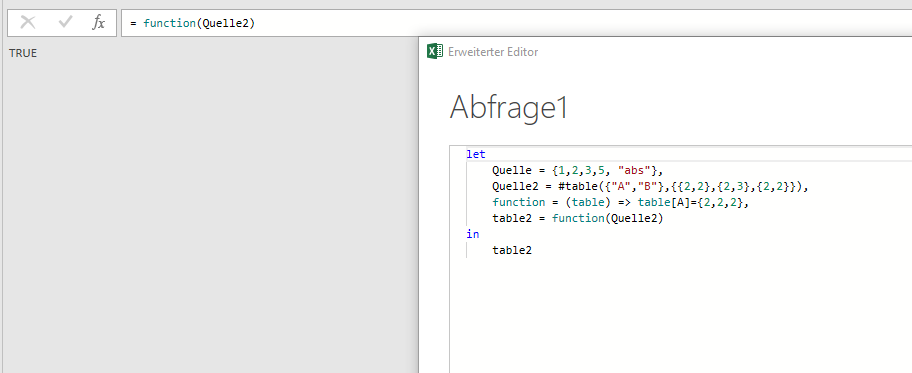
\includegraphics[scale = 0.3]{attachment/chapter_1/screenshot037}
	\caption{}
	\label{fig:screenshot037}
\end{figure}
Es sei vermerkt, es werden nicht die Typen abgefragt, sondern jeder Eintrag in der Liste wird verglichen.

\begin{figure}[H]
	\centering
	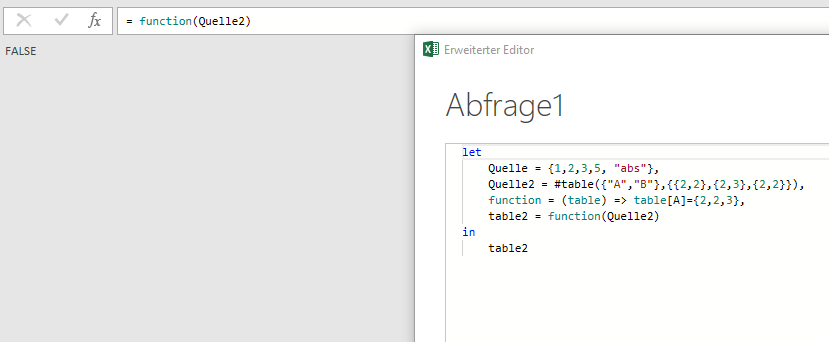
\includegraphics[scale = 0.3]{attachment/chapter_1/screenshot038}
	\caption{}
	\label{fig:screenshot038}
\end{figure}
Im Abschnitt \textbf{each} wir über die eine spezielle Funktion gesprochen. 
\subsection{Spezielle}
\subsubsection{Empty Variable}
Um den Ausdruck \textbf{each} verstehen zu können, sollte die Leere-Variable besprochen werden. In Phython als auch M wir $\_$ für Puffervariablen genutzt, welche später nicht mehr gebracht werden. 
\begin{lstlisting}[style=M]
let
	_ = Table.FromColumns({
		{"Fred", "Mary", "Phil", "Sue"},
		{1, 2, 3, 4},
		{5, 2, 5, 1}},
		{"Person", "Index", "Score"} // Tabellenkopf
	)
in
	_ // Die temporäre Variable heißt _ und ist vom Type table.
\end{lstlisting}

Um verschiedenen Daten von der Tabelle abzurufen, nutzen wir die Indexschreibweise:
\begin{align} 
	\text{Tabellen-Variablen-Namen}\left\lbrace\text{Zeile} \right\rbrace \left[\text{Spaltennamen}\right]
\end{align} 
Für den Variablennamen $\_$ gilt dies natürlich auch:
 \begin{lstlisting}[style=M]
let
	_ = Table.FromColumns({
		{"Fred", "Mary", "Phil", "Sue"},
		{1, 2, 3, 4},
		{5, 2, 5, 1}},
		{"Person", "Index", "Score"} // Tabellenkopf
	)
in
	_[Person] // Return Gesamte Spalte Person vom type list
	// _{2}[Person] // Return Zeile 2 der Spalte Person
\end{lstlisting}
Den temporären Variablennamen können wir auch weglassen, wenn Tabellen angesprochen werden. Dieser Prozess sollte für Listen nicht verwendet werden, da Power Query einen Zeilenverweis für Listen als neue Liste interpretiert:
 \begin{lstlisting}[style=M]
let
	_ = {"ab", null, 6}
in
	_{2} // Return null
	// {2} // Erstellen einer weiteren Liste
\end{lstlisting}

Für Tabellen kann jedoch der $\_$ weggelassen werden.

 \begin{lstlisting}[style=M]
let
	_ = Table.FromColumns({
		{"Fred", "Mary", "Phil", "Sue"},
		{1, 2, 3, 4},
		{5, 2, 5, 1}},
		{"Person", "Index", "Score"} // Tabellenkopf
	)
in
	[Person] // Return Gesamte Spalte Person
\end{lstlisting}
\subsubsection{Each}
Die Funktion \textit{each} ist eine einfache Funktion, welche die Syntax der Leeren Variable nutzt. Es gilt:
\begin{align}
\text{each }x := (\_) => \_ x 
\end{align} 
Der Begriff each ist vielleicht etwas irreführend, da nicht wirklich ein \textit{loop}-Durchlauf gestartet wird. Vielmehr wird die each-Funktion genutzt, wenn die ummantelnde Funktion den loop-Durchlauf startet und each eine Überprüfung für jede der übergebenen Element machen soll. \\

Es ist sehr wichtig zwischen Tabellen und Records zu unterscheiden. Wir der each-Funktion eine Tabelle übergeben und sie soll bewerten, ob eine Wert in jeder Zeile steht, funktioniert dies nicht mit einem einzelnen Wert

\begin{figure}[H]
	\centering
	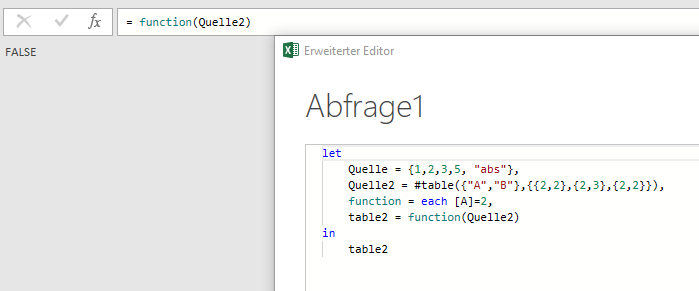
\includegraphics[scale = 0.3]{attachment/chapter_1/screenshot039}
	\caption{}
	\label{fig:screenshot039}
\end{figure}
Auch hier gilt, es muss mit einer Liste abgeglichen werden.

\begin{figure}[H]
	\centering
	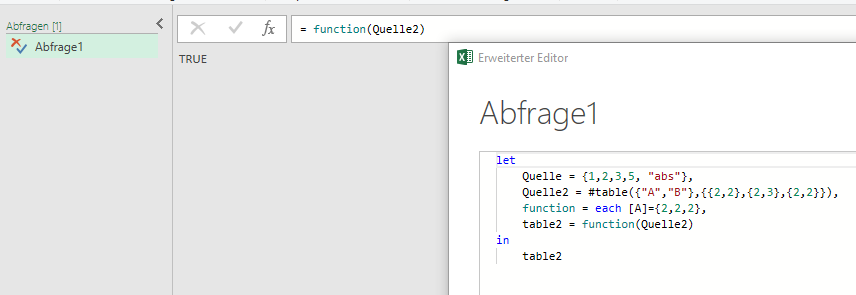
\includegraphics[scale = 0.3]{attachment/chapter_1/screenshot040}
	\caption{}
	\label{fig:screenshot040}
\end{figure}
Damit each \textit{true} zurückgeben kann, muss die geprüfte List ebenfalls die richtigen Wert enthalten.

\begin{figure}[H]
	\centering
	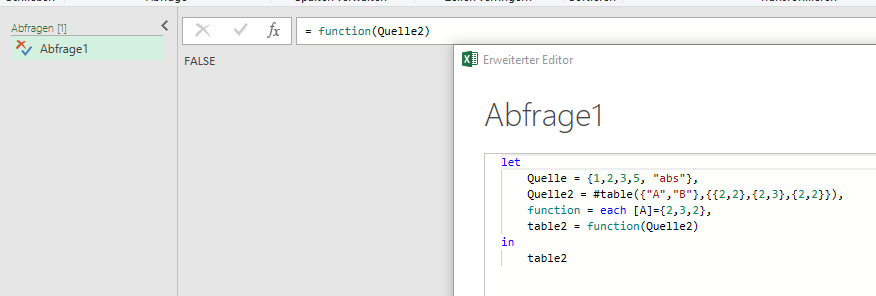
\includegraphics[scale = 0.3]{attachment/chapter_1/screenshot041}
	\caption{}
	\label{fig:screenshot041}
\end{figure}
Wird die Funktion \textbf{Table.SelectRows()} eingesetzt, so wir nicht eine Tabelle, sondern ein Record für die zu überprüfenden Zeile übergeben.

\begin{figure}[H]
	\centering
	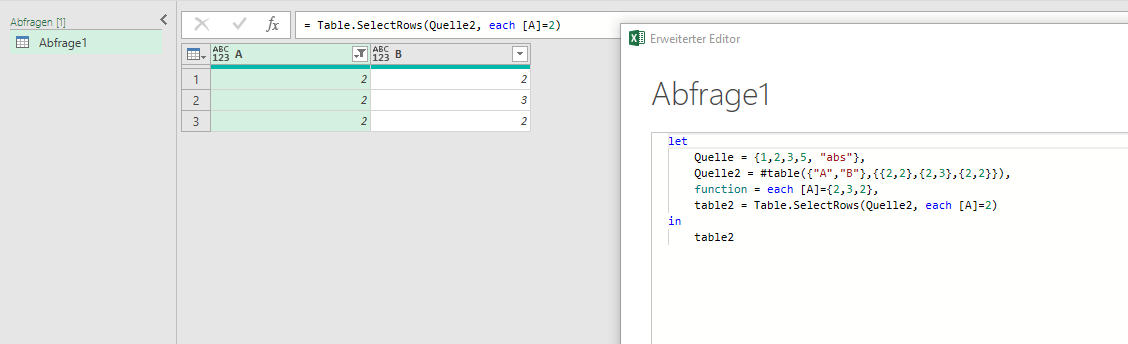
\includegraphics[scale = 0.3]{attachment/chapter_1/screenshot042}
	\caption{}
	\label{fig:screenshot042}
\end{figure}

Der \textit{each} Operator nimmt das übergebenen Record-Element, welches aus der Tabelle extrahiert wurde und überprüft mit der Eintragssyntax $[]$, die auch die Spaltensyntax für Tabellen ist, den Wert der für die Zeile in der entsprechenden Spalte steht. Eine einfache logsiche Abfrage entscheidet dann, ob der Eintrag zu $"$jeder$"$ Zeile in der entsprechenden Spalten richtig ist. Wenn ja, dann wird die Zeile ausgewählt, wenn nein, dann wird die Zeile gelöscht.\\
In der $Table.SelectRows()$ Funktion wir jede Zeile als Record übergeben. Wie oben beschrieben, wird die Auswahl pro Zelleninhalt ausgewertet.
\begin{figure}[H]
	\centering
	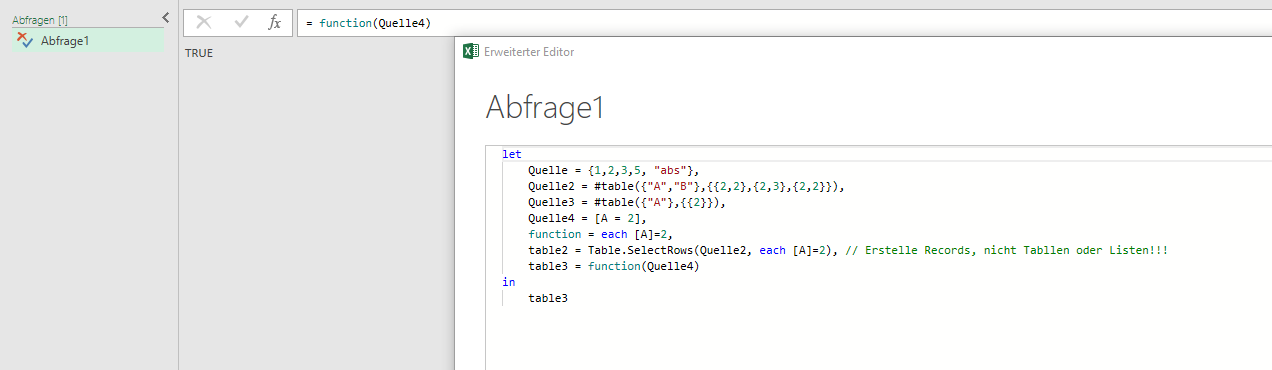
\includegraphics[scale = 0.3]{attachment/chapter_1/screenshot048}
	\caption{}
	\label{fig:screenshot048}
\end{figure} 

\subsubsection{try otherwise}
Das $\textit{try}\dots \textit{otherwise}$ Statment ist für besonders geeignet, um Fehler abzufangen. Wie das \textit{if-}Statment werden zwei Szenarien festgelegt, welche ausgeführt werden, nach der Überprüfung einer Bedingung. \\

Das try-otherwise Statment fängt jedoch \textit{Fehler} ab. Die Bedingung ist somit, wenn die Bedingung (Funktion) einen Fehler produziert, dann wird \textit{otherwise} ausgeführt.


\section{Business Intelligence: Part I - Power Query} 
\subsection{Introduction to Excel Tools}
Im ersten Teil des Kurses wird besprochen welche Methoden es in der Microsoft Power BI Umgebung gibt. In der Business Version sind einzelne Komponenten integriert, welche vollintegriert in der BI-Version sind. \\ 
In der Übersicht wird gezeigt, wie die einzelnen Komponenten aufgebaut sind.
\begin{figure}[H]
	\centering
	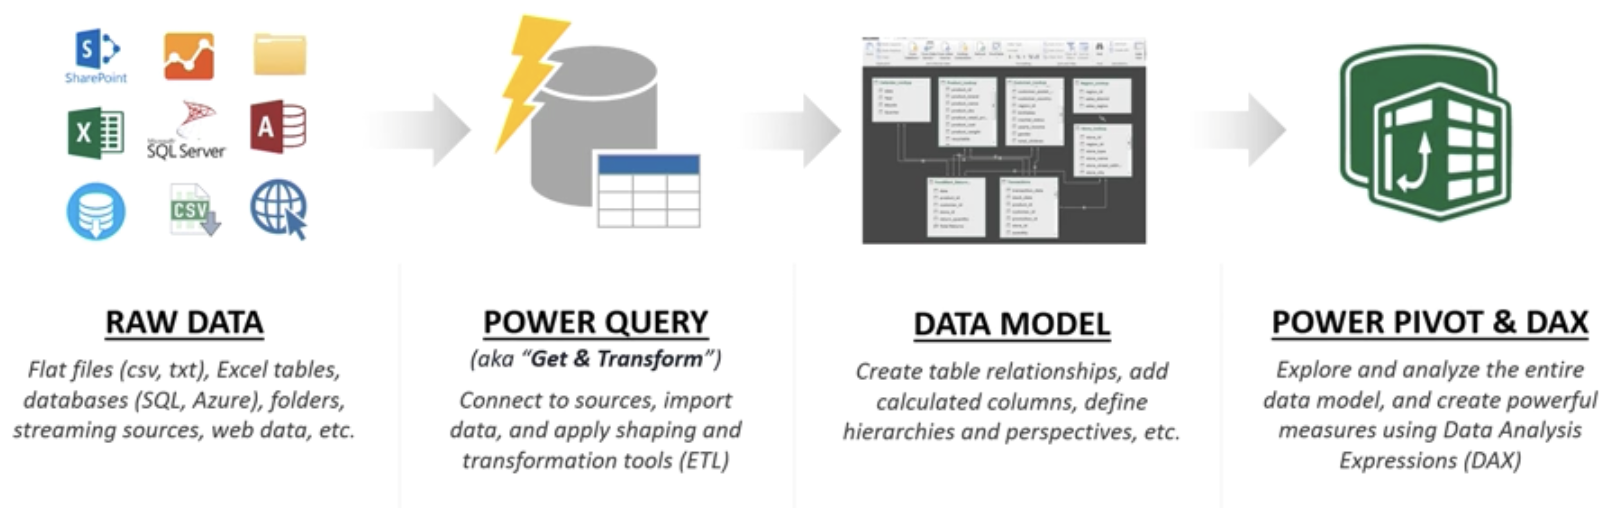
\includegraphics[scale = 0.3]{attachment/chapter_1/screenshot019}
	\caption{}
	\label{fig:screenshot019}
\end{figure}
\begin{description} 
\item[Datenbank] 
\begin{itemize}
\item Access wird mehr als Datenbank gesehen. Welche Fragen noch offen sind, im Hinblick auf Power Query, ist: "Wie unterscheiden sich Access Queries von Power Query-Abfragen?". 
\item Weitere Datenspeicherungen können in \gls{csv} oder \gls{xlsx} Dateien liegen.
\item Es können aber auch Server wie SQL Server oder SharePoint angebunden werden.
\end{itemize}
\item[Query] Mit Hilfe der Abfragen können spezifische Fragen an die eingelesenen Daten gestellt werden. Diese werden in Excel geladen. Entweder werden die Daten direkt in Excel eingelesen und oder über Pivot Tabellen / Charts dargestellt oder sie können in das Datenmodell eingelesen werden. Per Query wird mit Prinzip \gls{ETL} gearbeitet. 
\item[Datenmodell] In dem Datenmodell werden Beziehungen zwischen verschiedenen Datenquellen oder spezifischer Tabellen bezogen. Die Daten werden mit einen speziellen Komprimierungsverfahren gespeichert. Gespeichert werden die Daten im Arbeitsspeicher, für die weitere Verarbeitung. Ergänzend zur Queries durch Power Query können auch weitere Spalten angefügt werden. Es ist wichtig zu vermerken, dass nur die Daten im Datenmodell gespeichert werden, die entweder selektiert durch die Query eingelesen wird oder direkt eingespeichert wird. 
\item[PowerPivot] Dieses Option umfasst nicht nur die dynamischen Pivottabellen sondern auch die \textbf{Measures}. Power Pivot verwaltet nicht nur eine einfache Tabelle, sondern greift auf das komplette Datenmodell zu. Mit Measures können BI-Funktionen geschaffen werden. Diese werden mit \gls{DAX} erstellt.
\end{description}

\subsection{Query Editor - Tabellenblätter}
Power Query bietet verschiedene Möglichkeiten an, Daten in Excel zu laden. 
\begin{figure}[H]
	\centering
	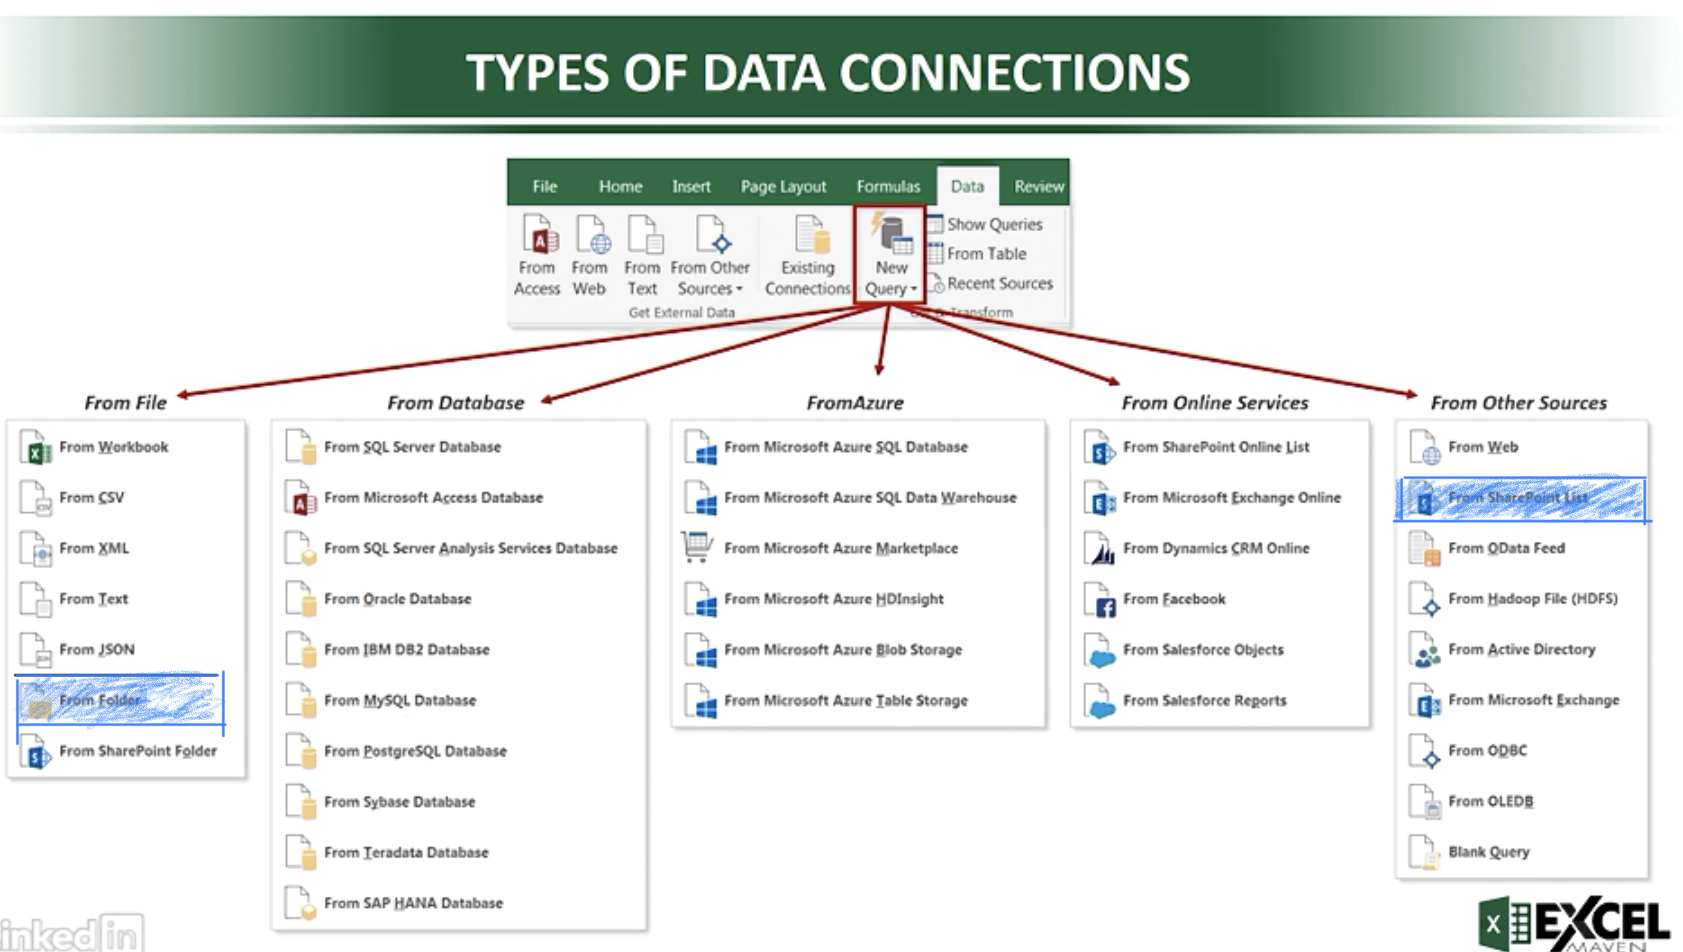
\includegraphics[scale = 0.3]{attachment/chapter_1/screenshot020}
	\caption{}
	\label{fig:screenshot020}
\end{figure}
Im ersten markierten Bereich wird drauf verwiesen, einen Pointer auf einen Ordner zeigen zu lassen. Ebenso ist es möglich, eine SharePoint-Seite anzusprechen.\\ 

Der Editor ist in drei Bereiche eingeteilt: \begin{figure}[H]
	\centering
	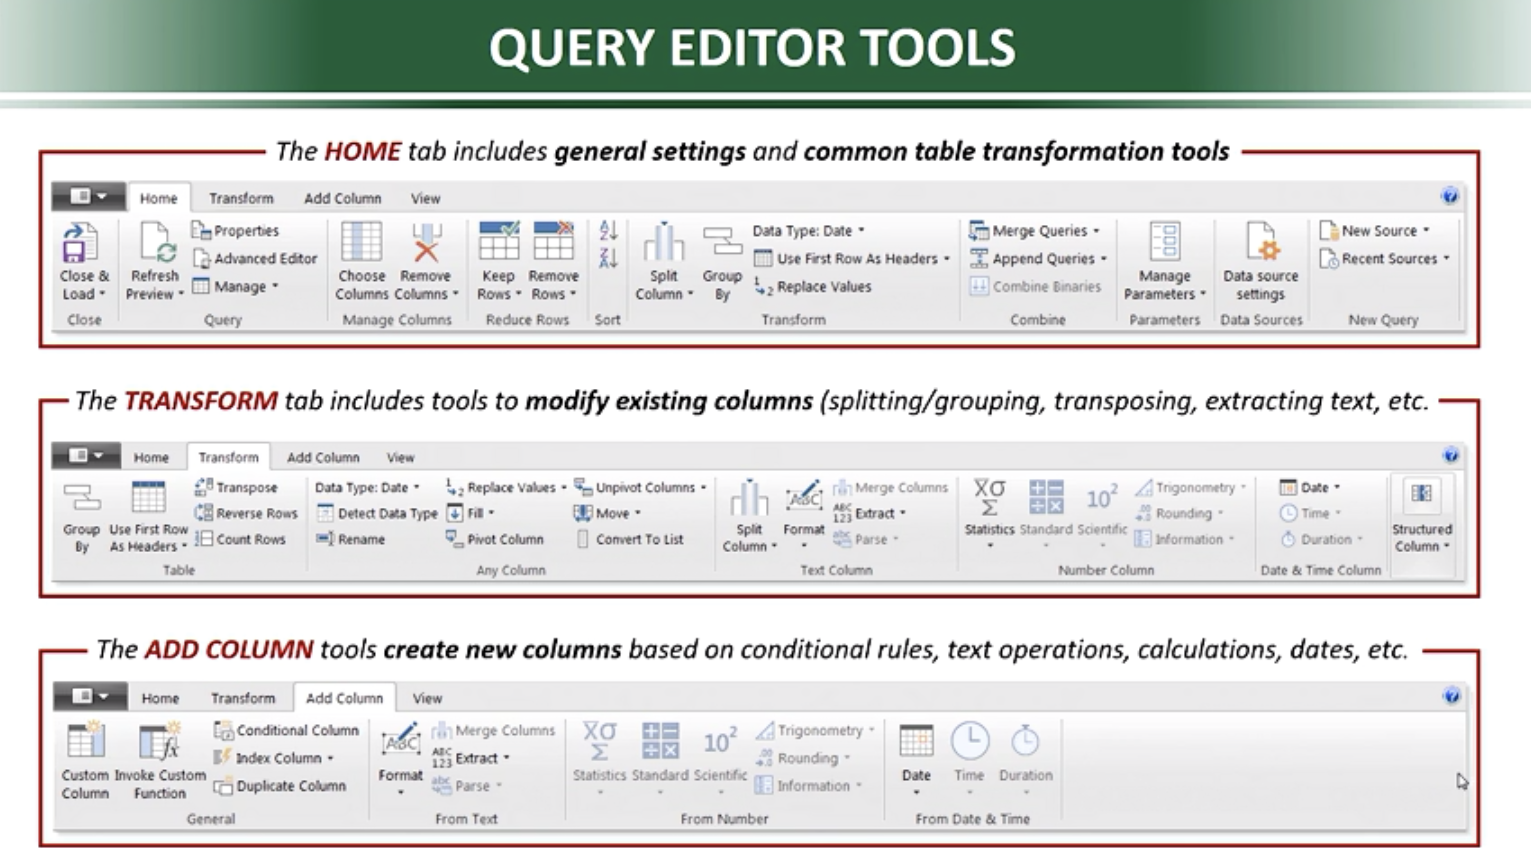
\includegraphics[scale = 0.3]{attachment/chapter_1/screenshot021}
	\caption{}
	\label{fig:screenshot021}
\end{figure}
\begin{itemize}
\item Home: Die Daten sind geladen und werden transformiert. 
\item Transform: Die Daten sind geladen und werden transformiert $\&$ verändert.
\item Add Column: Die Daten sind geladen und werden transformiert $\&$ neue Daten werden angefügt.
\end{itemize}
\subsubsection{Home}
\begin{description}
\item[Remove Duplicates] Dies Funktion ist nützlich, wenn man dynamische Indexfunktion erstellen will. Zum Beispiel, kann für die 
\begin{figure}[H]
	\centering
	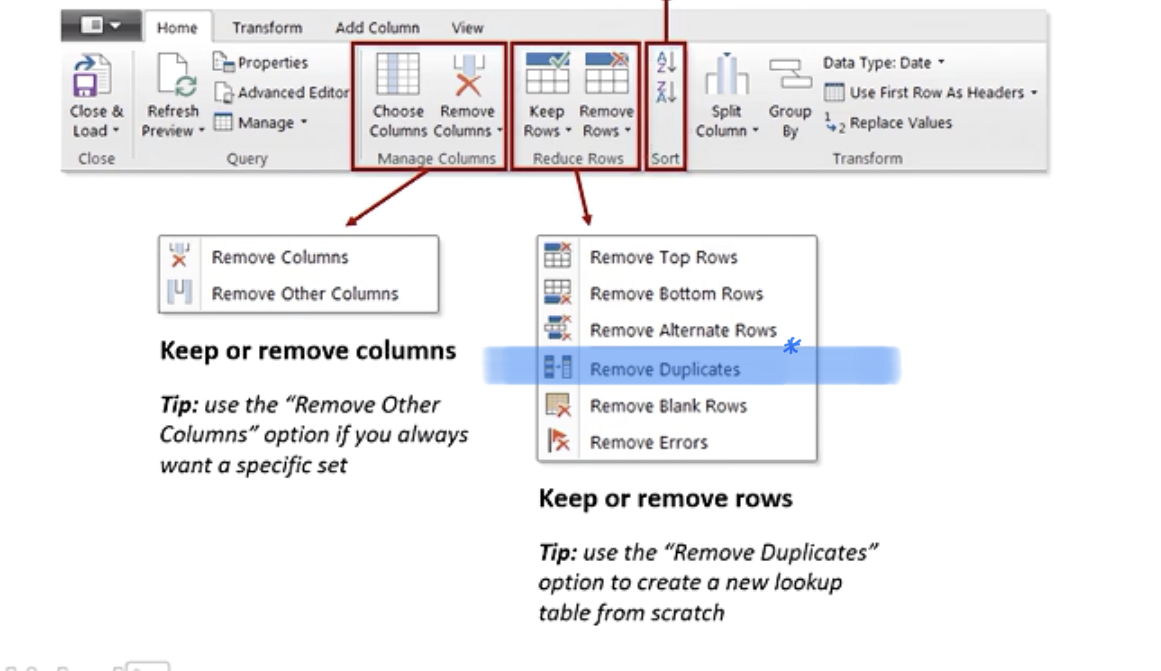
\includegraphics[scale = 0.3]{attachment/chapter_1/screenshot022}
	\caption{}
	\label{fig:screenshot022}
\end{figure}
\item[Proper Name] Es wird empfohlen die Queries auch als solche zu bezeichnen. Zum Beispiel $"$ETLName$"$. Dies wird sich (vermutlich) bei Power Pivot erschließen.
\begin{figure}[H]
	\centering
	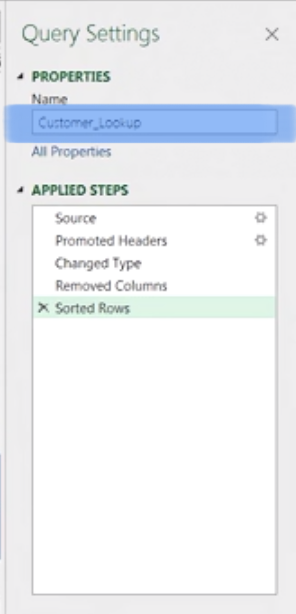
\includegraphics[scale = 0.3]{attachment/chapter_1/screenshot023}
	\caption{}
	\label{fig:screenshot023}
\end{figure}
\end{description}
\subsubsection{Transform}
\begin{description}
\item[Text Transformation] In dem Bereich unter dem Tab können Text-Einträge verändert werden. Die Funktionalität richtet sich vorrangig an Spalten vom String Typ. 
\begin{itemize}
\item Trim - Leerzeichen vor dem Eintrag können gelöscht werden.
\item Prefix - Textteile können angefügt werden.
\item Groß- und Kleinschreibung kann angepasst werden
\item Beispiel: Die Namen in der Liste können angepasst werden, falls die Vor- und Nachnamen nicht richtig großgeschrieben sind. 
\end{itemize}
\begin{figure}[H]
	\centering
	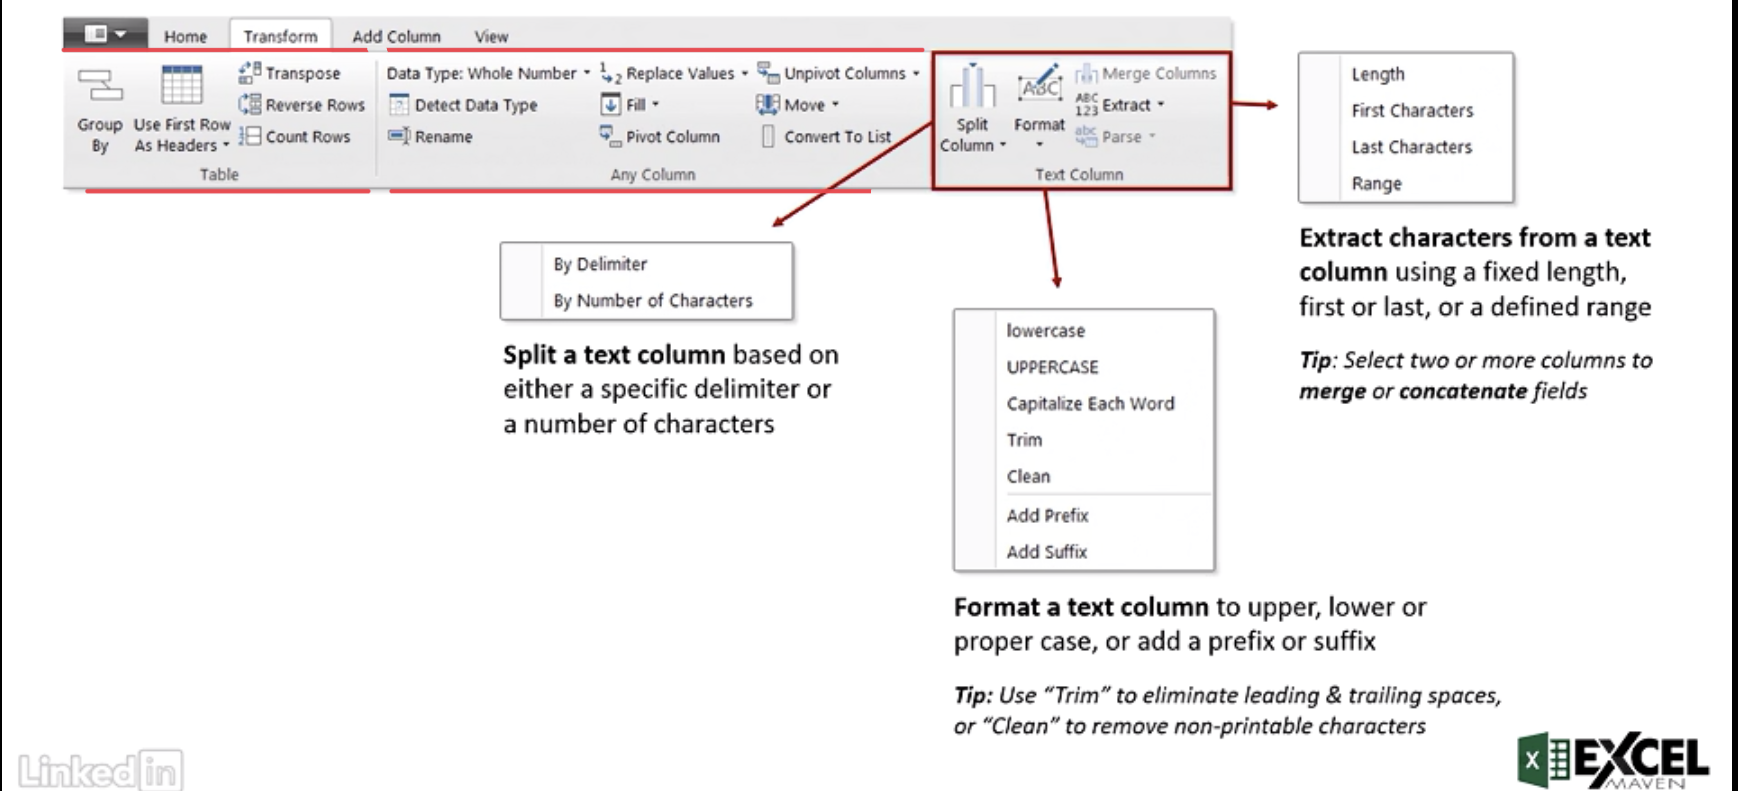
\includegraphics[scale = 0.3]{attachment/chapter_1/screenshot024}
	\caption{}
	\label{fig:screenshot024}
\end{figure}
\item[Zahlen Transformation]
\begin{itemize}
\item Statistiken geben Werte zurück. Eine oder mehrere Spalten werden reduziert auf einen Wert. Die Statistik-Funktionen werden nicht in dem \textit{Add Column} Tabellenblatt angezeigt. \textbf{Idee:} Statistik können bestimmt werden und per Verbingung gespeichert werden. Daraufhin werden diese in Power Pivot verwendet, um mit ihnen weiter zu rechnen. Den Wert kann in eine \textit{Liste} oder eine \textit{Tabelle} konvertieren.
\begin{figure}[H]
	\centering
	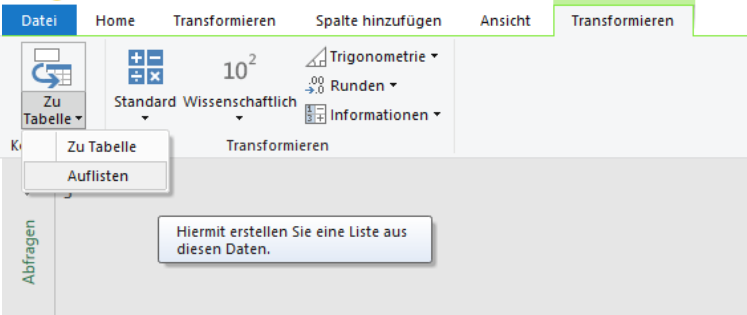
\includegraphics[scale = 0.3]{attachment/chapter_1/screenshot026}
	\caption{}
	\label{fig:screenshot026}
\end{figure}
\item Standard, Wissenschaftliche oder andere Funktion für numerische Spalten lassen sich auf Spalten anwenden
\end{itemize}
\begin{figure}[H]
	\centering
	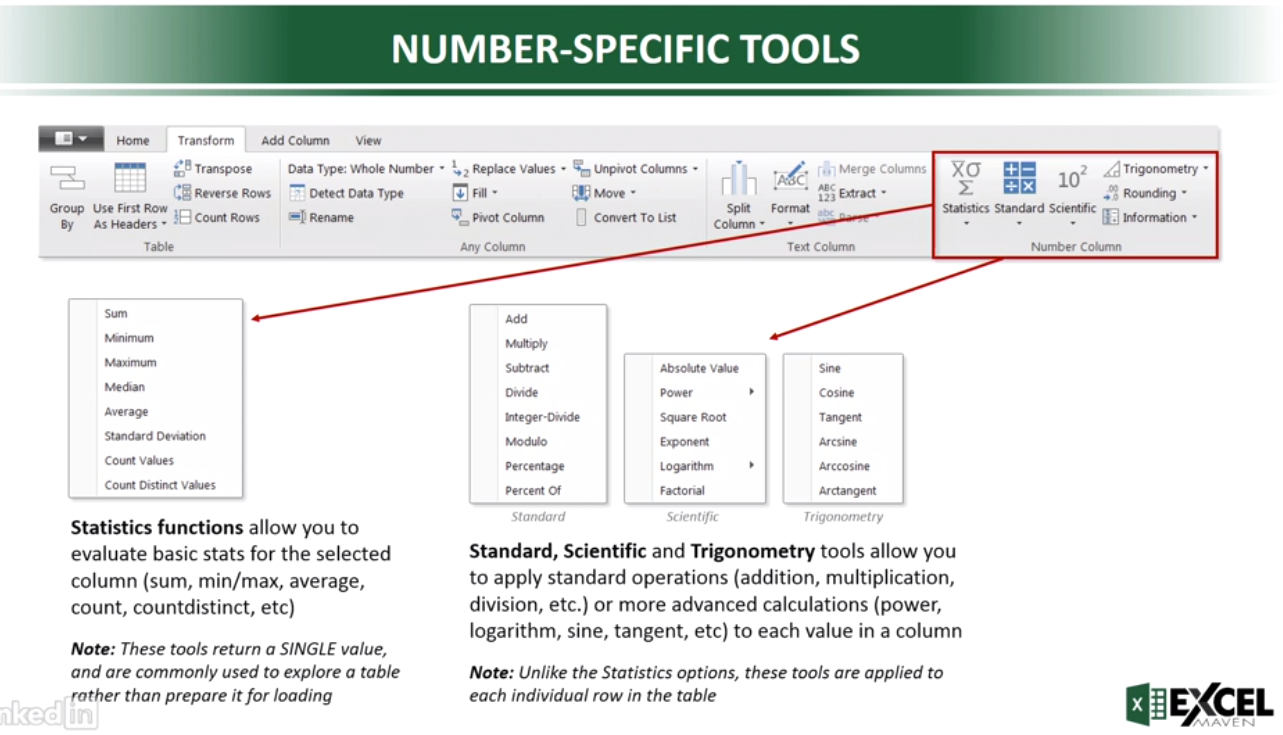
\includegraphics[scale = 0.3]{attachment/chapter_1/screenshot025}
	\caption{}
	\label{fig:screenshot025}
\end{figure}
\item[List Tool] Die Werte der Tabelle können nicht direkt verändert werden. Es kann nicht einfach in eine Zelle gegangen werden und ein Wert verändert werden. Mit List können aber ganz neue Spalten, von einer Satt aus, erstellt werden. 
\begin{itemize}
\item Power M - List - Funktionen (siehe Dokument)
\begin{figure}[H]
	\centering
	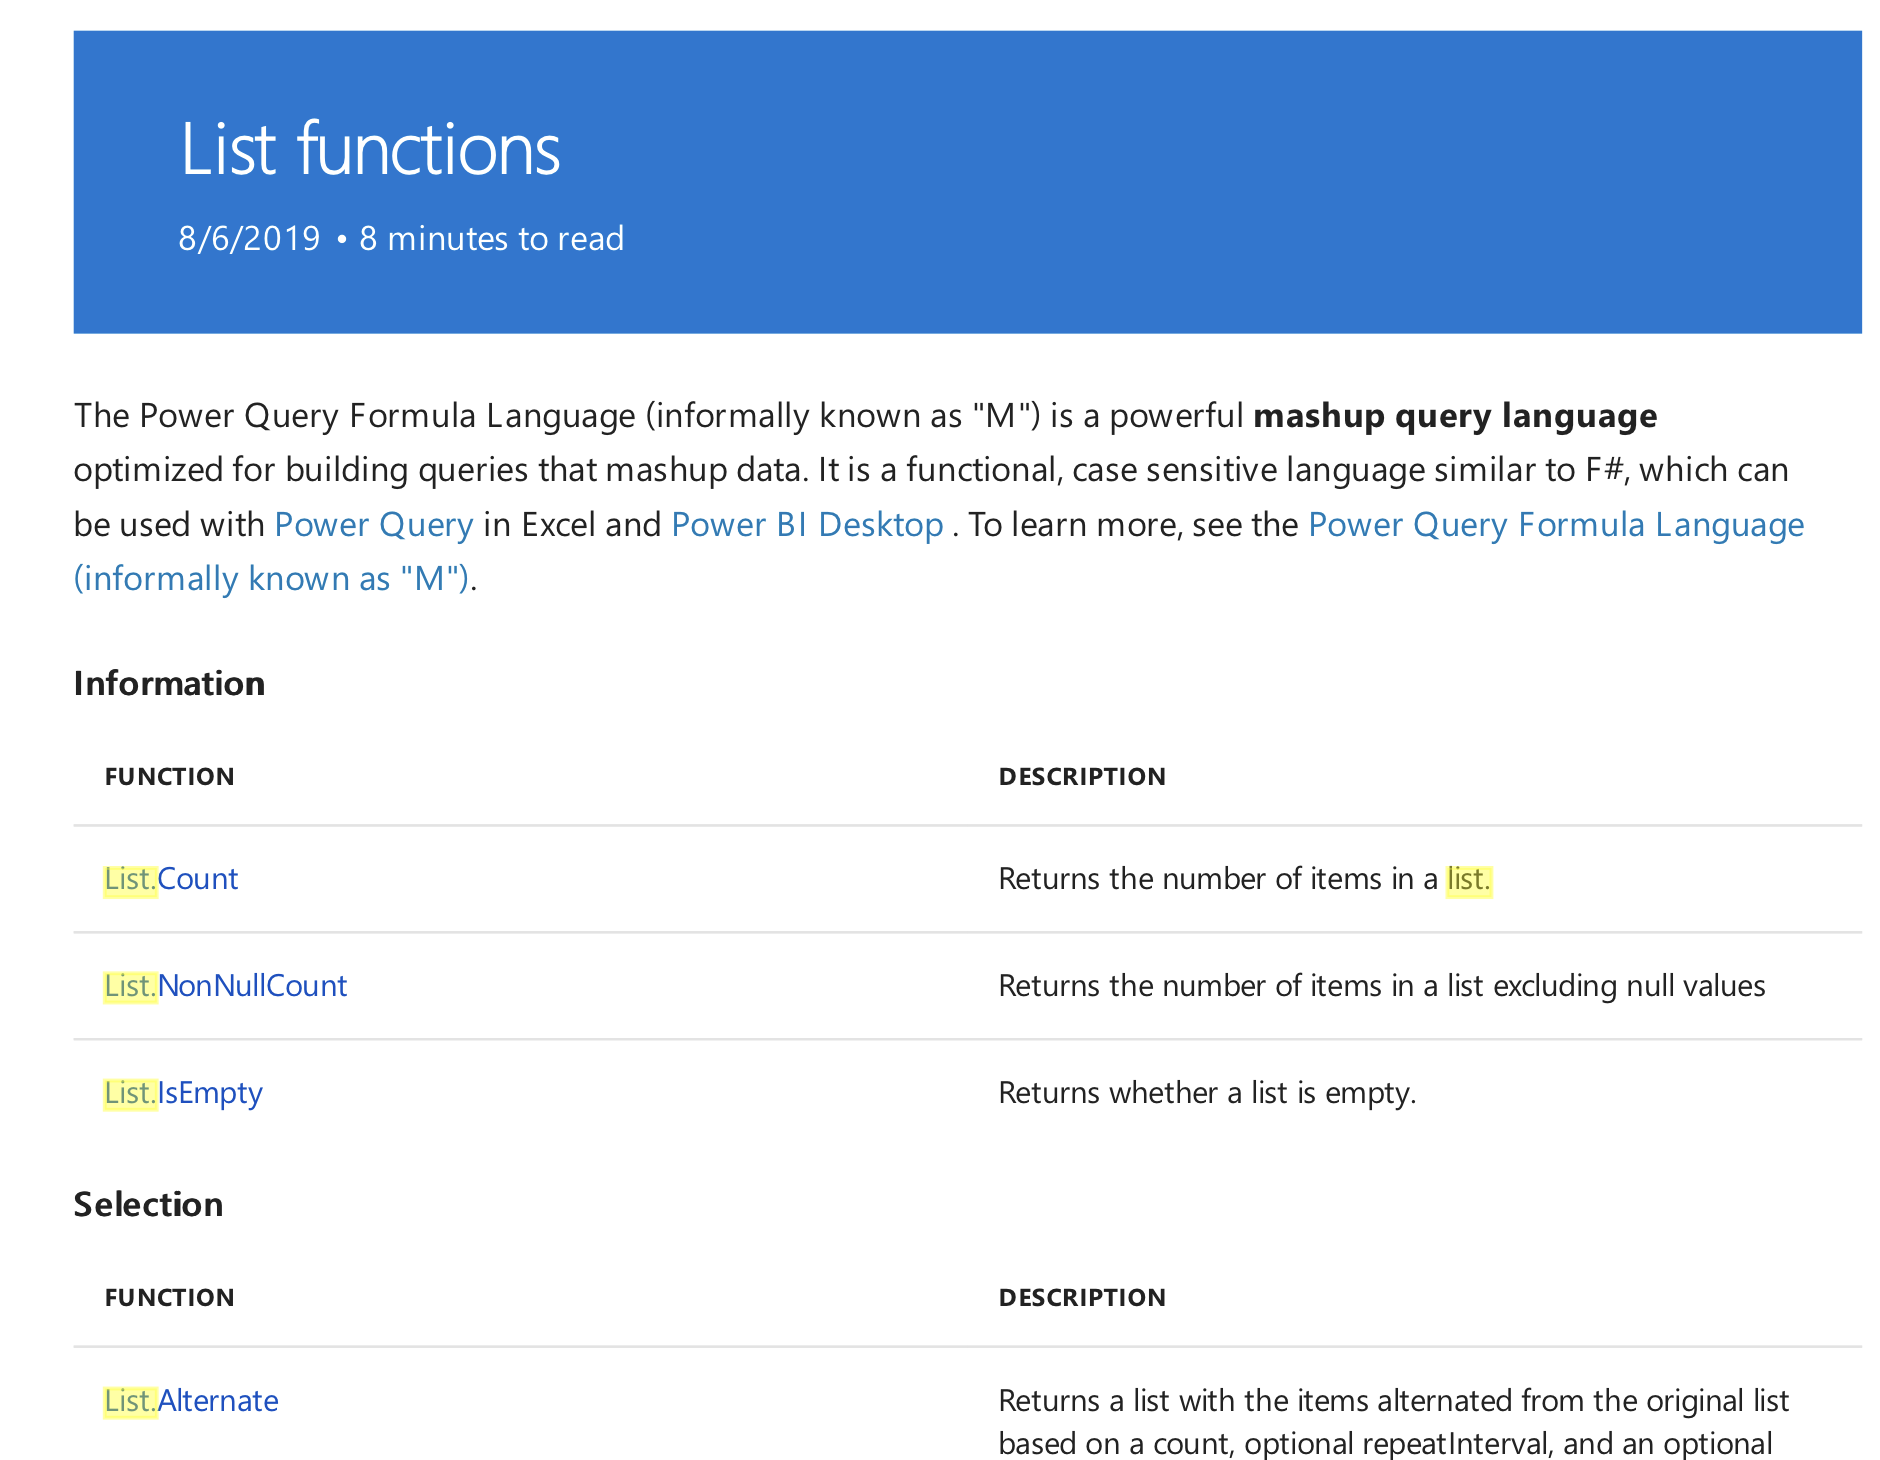
\includegraphics[scale = 0.3]{attachment/chapter_1/screenshot027}
	\caption{}
	\label{fig:screenshot027}
\end{figure}
\item Auch hier kann man keine einzelnen Zellen verändern.
\end{itemize}
Wie kann man eine neue Tabelle in Power Query anlegen?
\begin{itemize}
\item Offen \textit{Blank Power Query}
\item Mit der Funktion $=\#date(2017,1,1)$ wird der erste Eintrag in die Liste gemacht.
\begin{figure}[H]
	\centering
	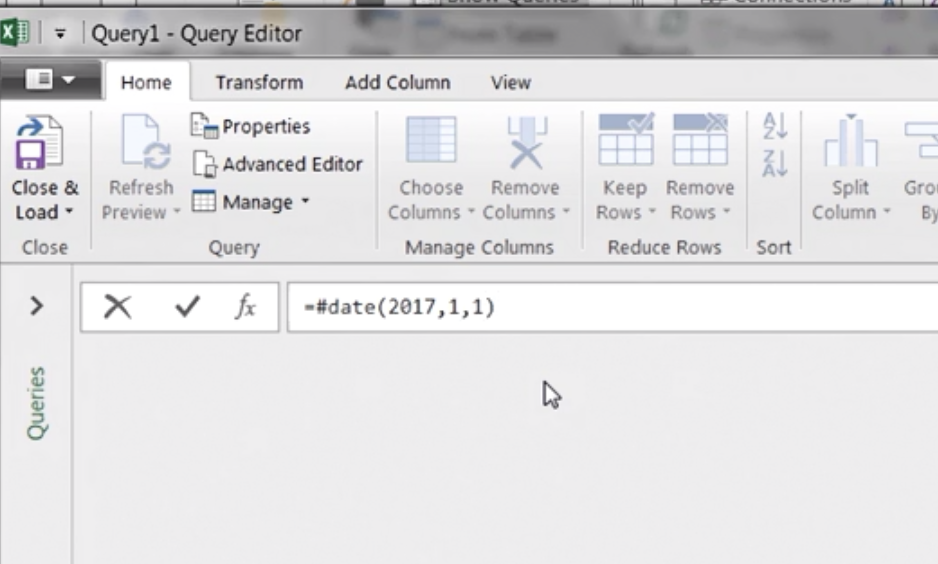
\includegraphics[scale = 0.3]{attachment/chapter_1/screenshot028}
	\caption{}
	\label{fig:screenshot028}
\end{figure}
Variablen werden in Power Query mit einem $\#$ begonnen.
\begin{figure}[H]
	\centering
	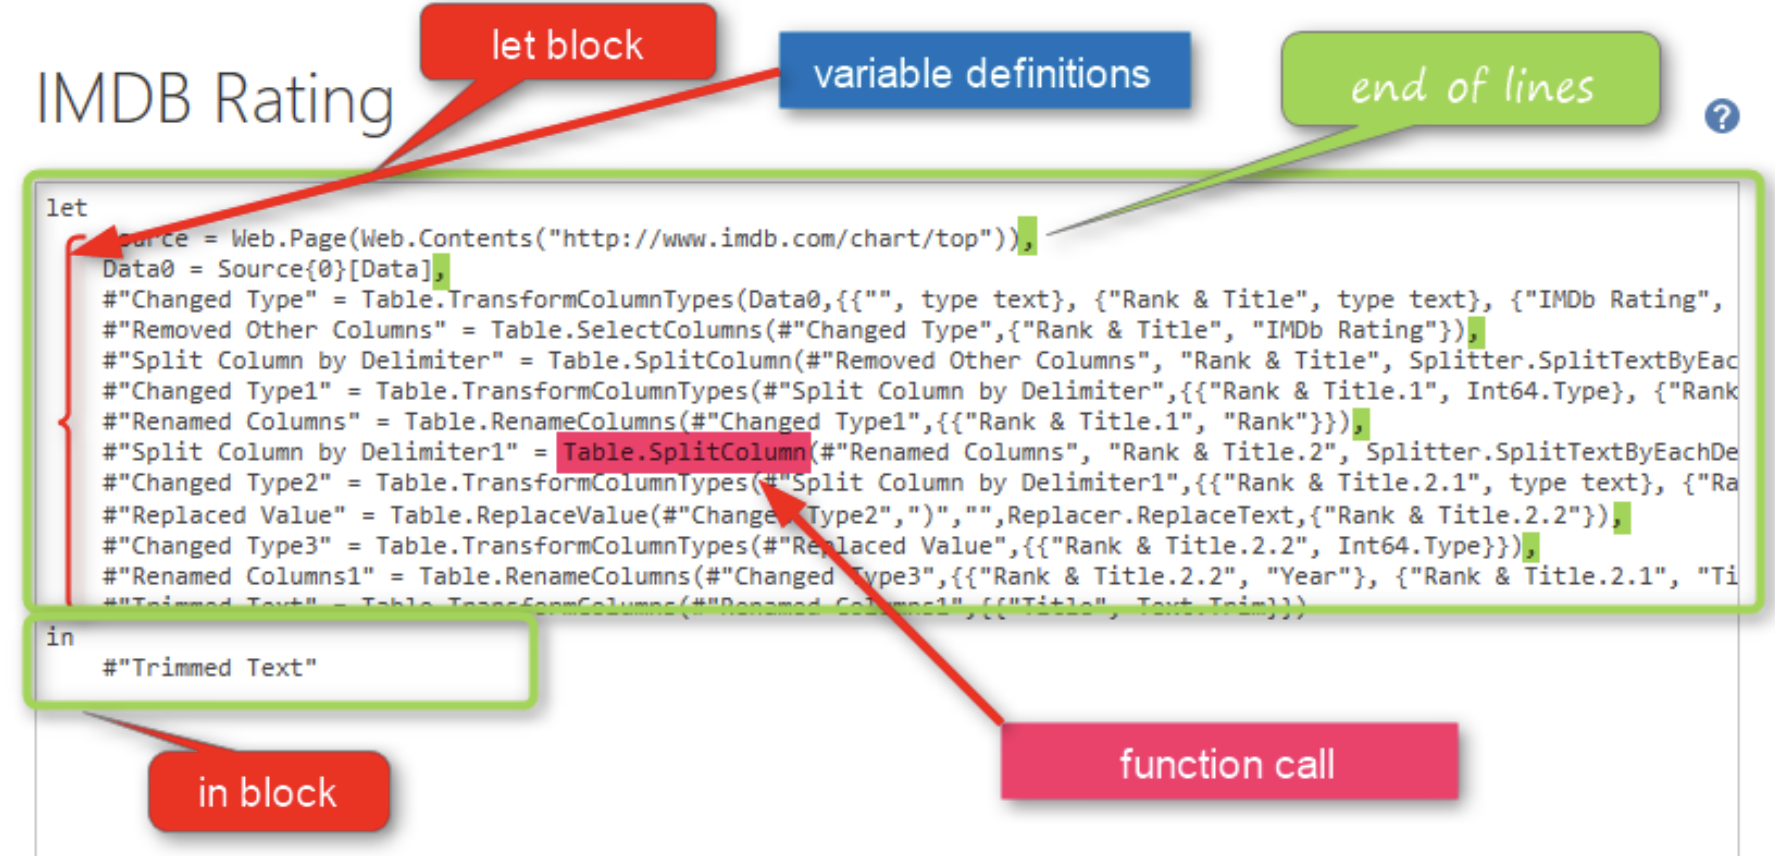
\includegraphics[scale = 0.3]{attachment/chapter_1/screenshot029}
	\caption{}
	\label{fig:screenshot029}
\end{figure}
Einfache Rechenoperationen sind auch möglich.
\end{itemize}
\end{description}

\section{Business Intelligence: Part II - Data Modeling 101}
\subsection{Data Normalization}
 Um Datenmodell aufzubauen, ist es sinnvoll, dem Prinzip der \textbf{Seperatierung} zu folgen. Daten die auf Sachverhalte mit verschiednen Entstehungsgründen zurückzuführen sind, sollten auch in seperate Tabellen stehen.
 

\begin{figure}[H]
	\centering
	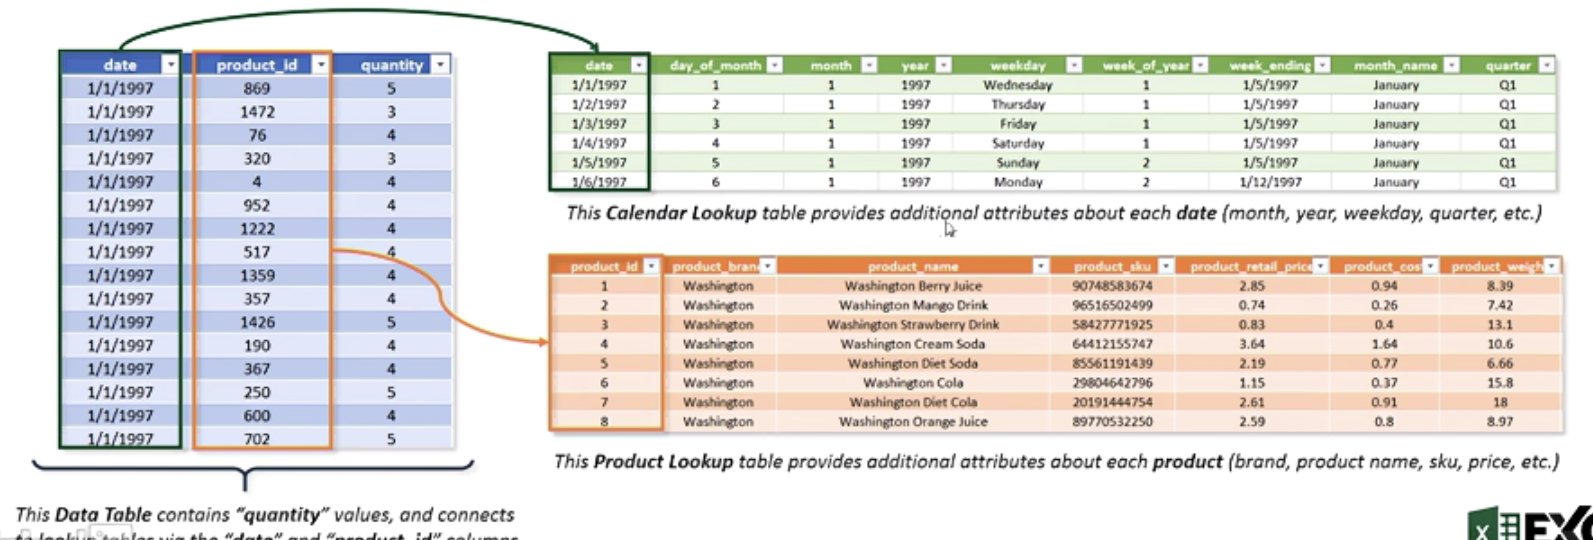
\includegraphics[scale = 0.3]{attachment/chapter_1/screenshot046}
	\caption{}
	\label{fig:screenshot046}
\end{figure}

In dem Beispiel sieht man, das die ergänzenden Daten zu dem Produkt in einer seperaten Tabelle gespeichert werden sollte.\\ 
Wir können ebenfalls unterscheiden, zwischen \textbf{Daten Tabellen} und \textbf{LookUp table}. Was als Vermerk angebracht wird, ist sich Kalender Tabellen zu generieren. Dies ist deshalb sinnvoll, weil Power Pivot kein so leichte Oberfläche hat, wie Power Query um Daten zu extrahieren (Bis jetzt).

\subsection{Data Model}

\subsubsection{Primary and Foreign Key}
The primary key serves as a unique identifier. The foreign key allows to connect to the primary key.

\begin{figure}[H]
	\centering
	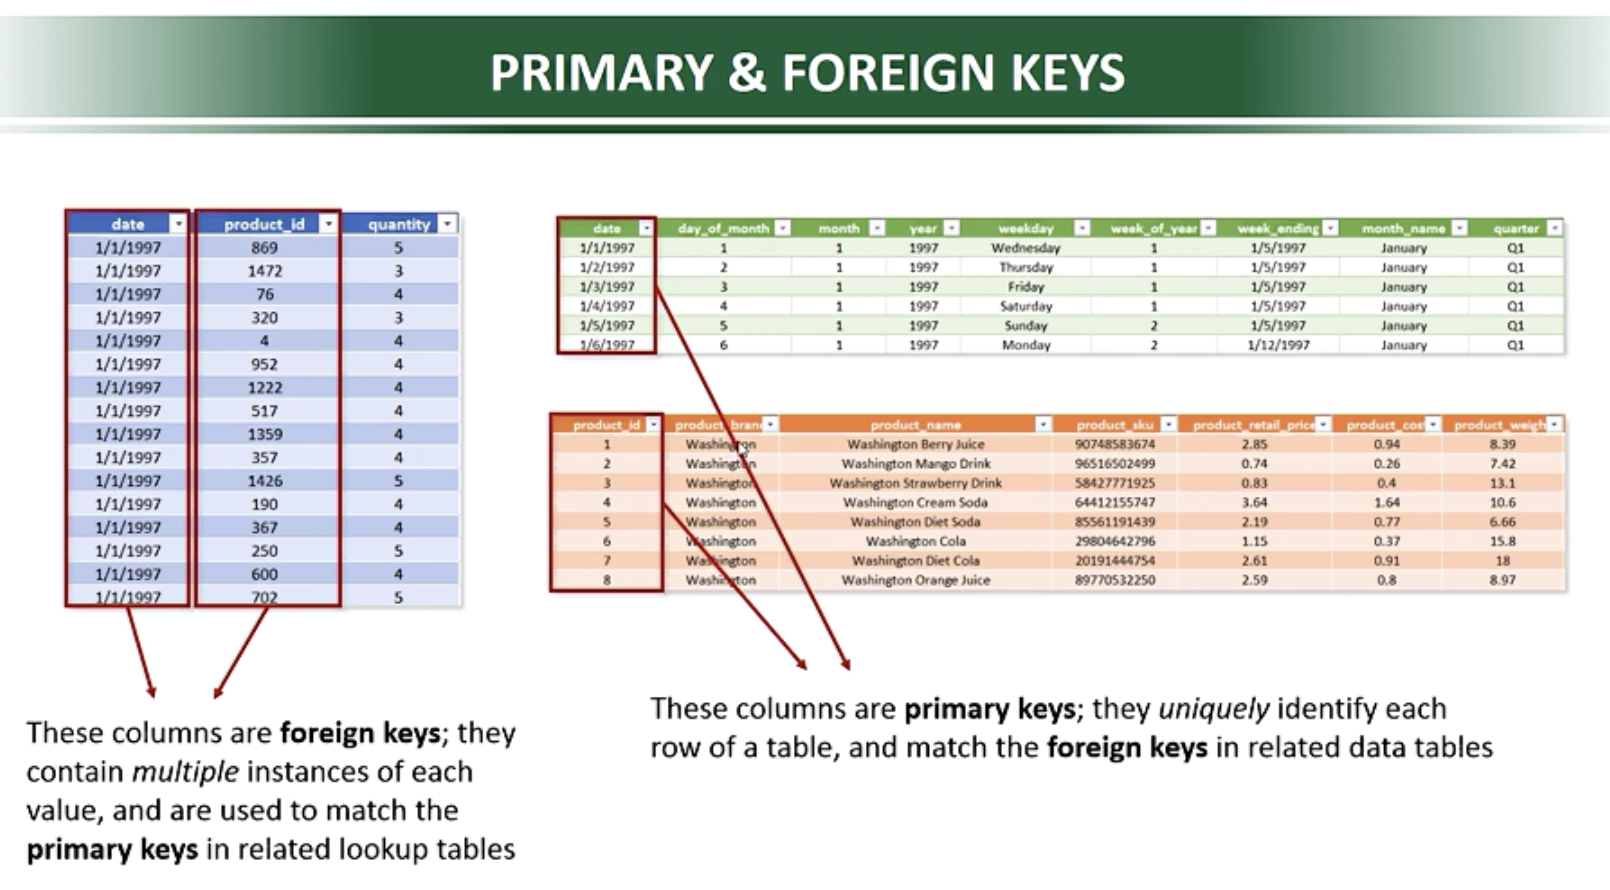
\includegraphics[scale = 0.3]{attachment/chapter_1/screenshot047}
	\caption{}
	\label{fig:screenshot047}
\end{figure}


Im Datendiagramm werden Beziehungen zwischen foreign und primary key gelegt. Dabei zieht man vom forgein key feld auf das primary key feld.\\ 

Welche andere Variante funktioniert, ist unter \textit{Design} zu sehen. Dabei erstellt man Beziehungen zwischen den Tabellen. Dies ist in Anlehnung an Power Query Zusammenführung.
\begin{figure}[H]
	\centering
	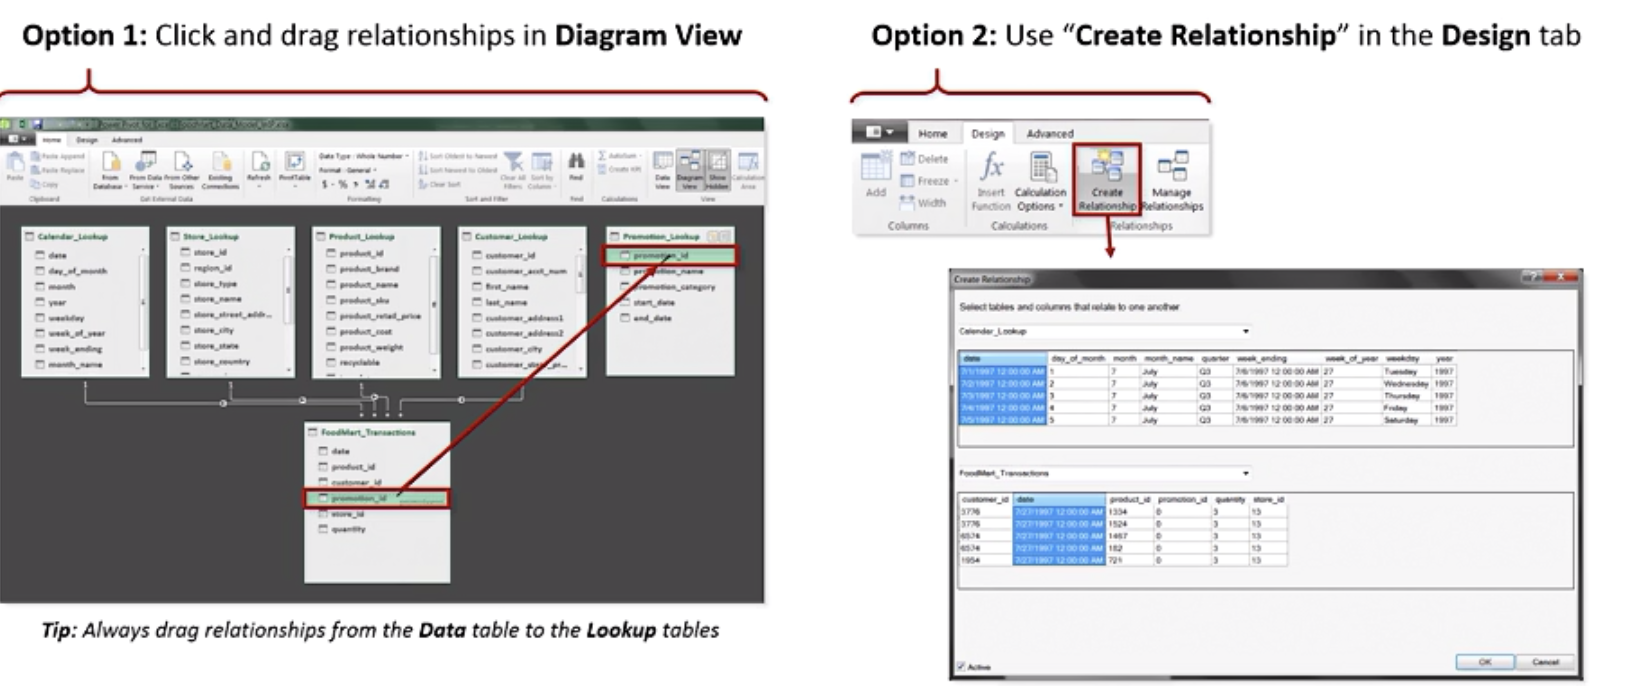
\includegraphics[scale = 0.3]{attachment/chapter_1/screenshot045}
	\caption{}
	\label{fig:screenshot045}
\end{figure}
\subsubsection{Beziehungen}
Beziehungen können auf zwei Arten erstellt werden. Die Beziehungen kann über die \textit{Diagramm Ansicht}, durch ziehen der Einträge, erstellt werden. Zum anderen kann eine Beziehungen auch über den Entwurf-Tab erstellt werden

\begin{figure}[H]
	\centering
	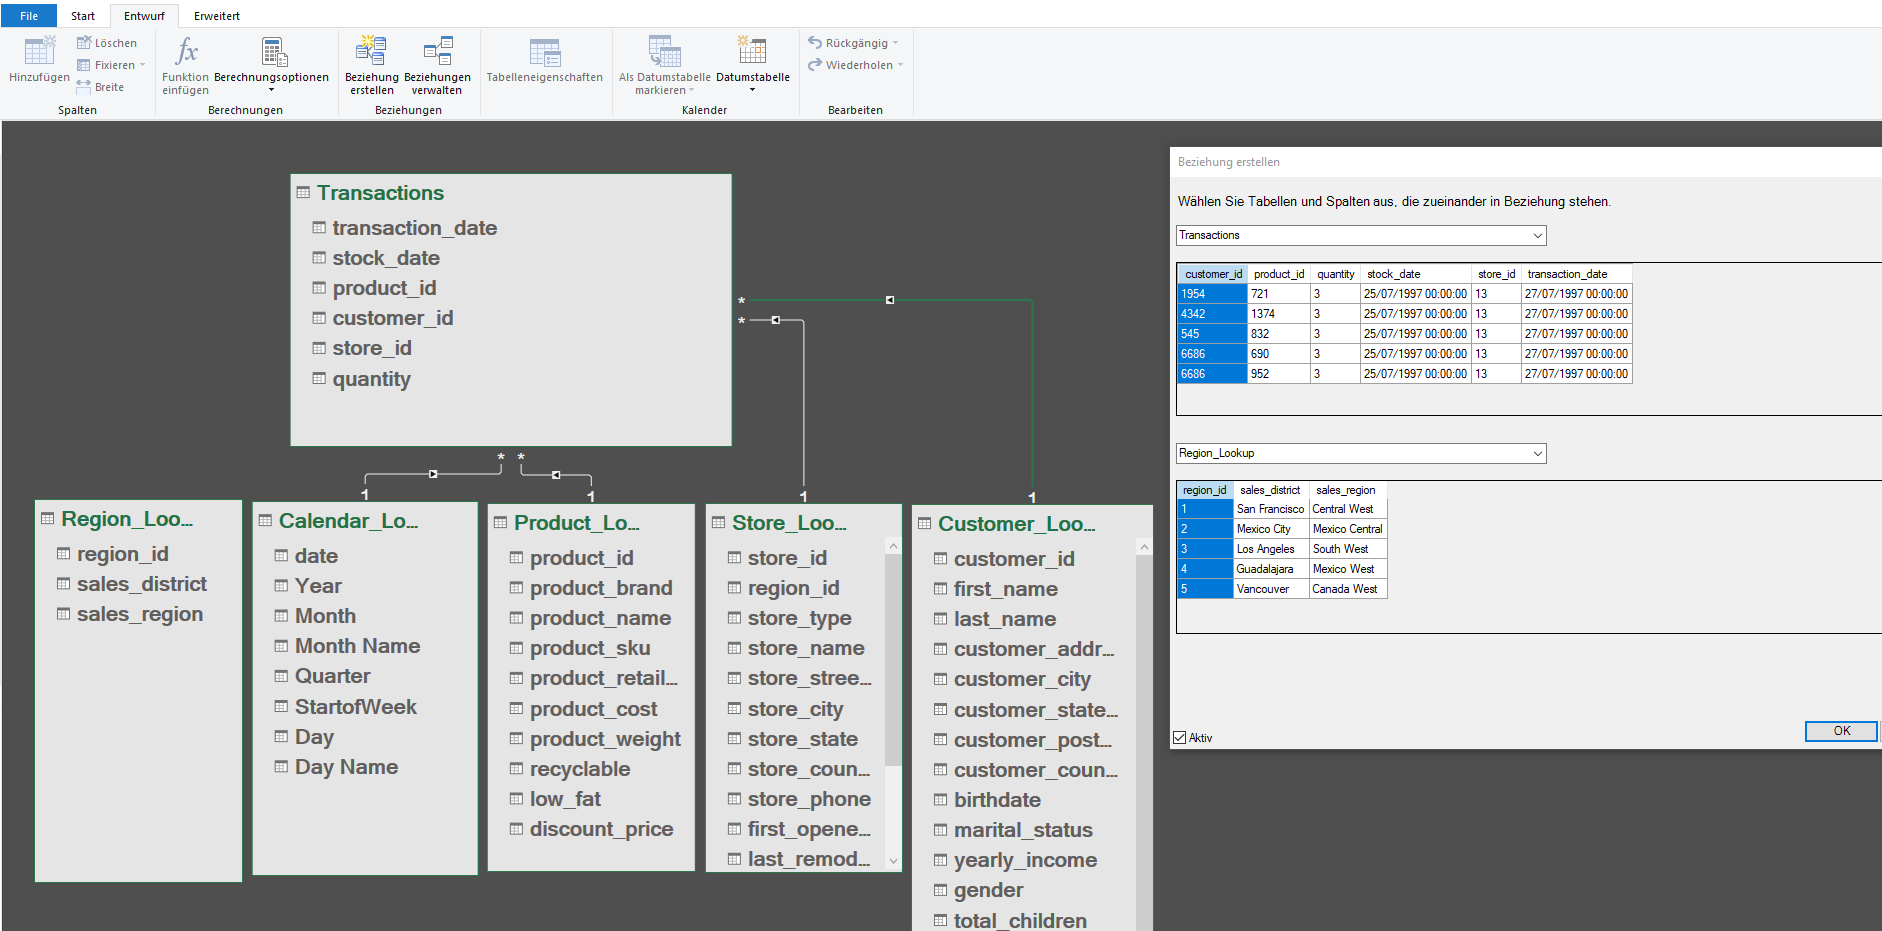
\includegraphics[scale = 0.3]{attachment/chapter_1/screenshot057}
	\caption{}
	\label{fig:screenshot057}
\end{figure}
In Power Query können verschiedene Schnittmengen gebildet werden. Es wird von \textit{Merge} gesprochen. Es können jedoch nur $n:1$ Beziehungen erstellt werden. Eine $m:n$ Beziehung von Power Pivot aktuelle nicht zur Verfügung gestellt. In Power Pivot kann nur eine Beziehungen zwischen zwei Tabellen erstellt werden. Eine weitere Beziehung wird dann als \textit{inaktiv} verwaltet. Im Datendigramm wird dies mit einer gestrichelten Linie angezeigt.
\begin{figure}[H]
 	\centering
	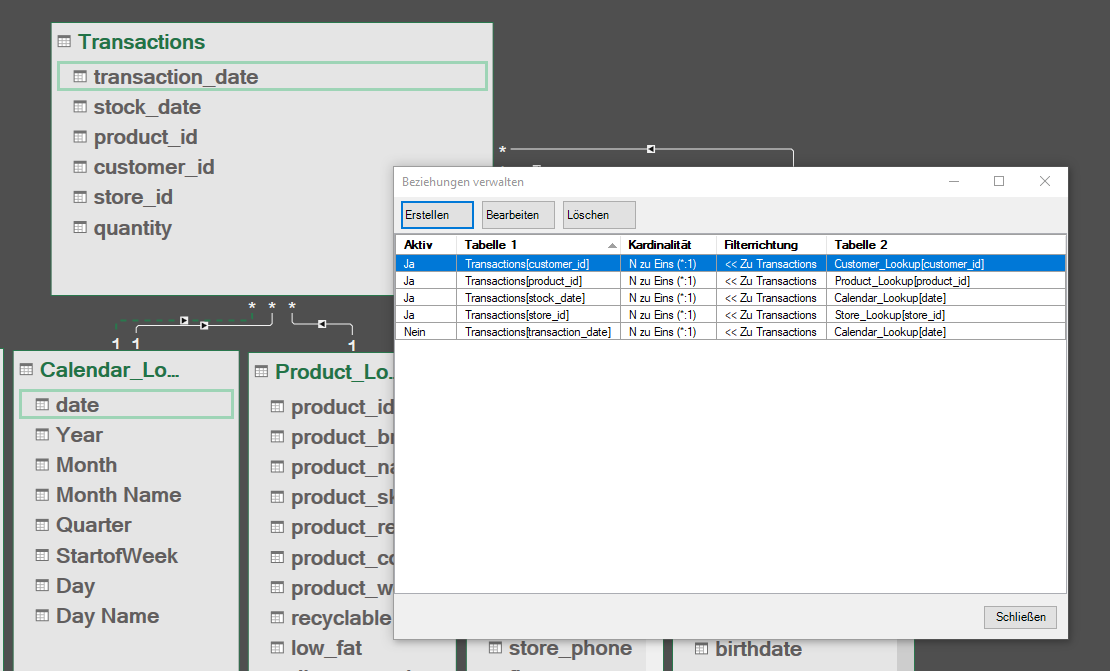
\includegraphics[scale = 0.3]{attachment/chapter_1/screenshot058}
	\caption{}
	\label{fig:screenshot058}
\end{figure}
\paragraph{Star Model}
In einem \textit{star model} werden Beziehungen nur zwischen \textit{primary key} Tabellen und \textit{foreign key} Tabellen erstellt. Es bildet sich einen Sternenmuster aus Beziehungen heraus.\begin{figure}[H]
	\centering
	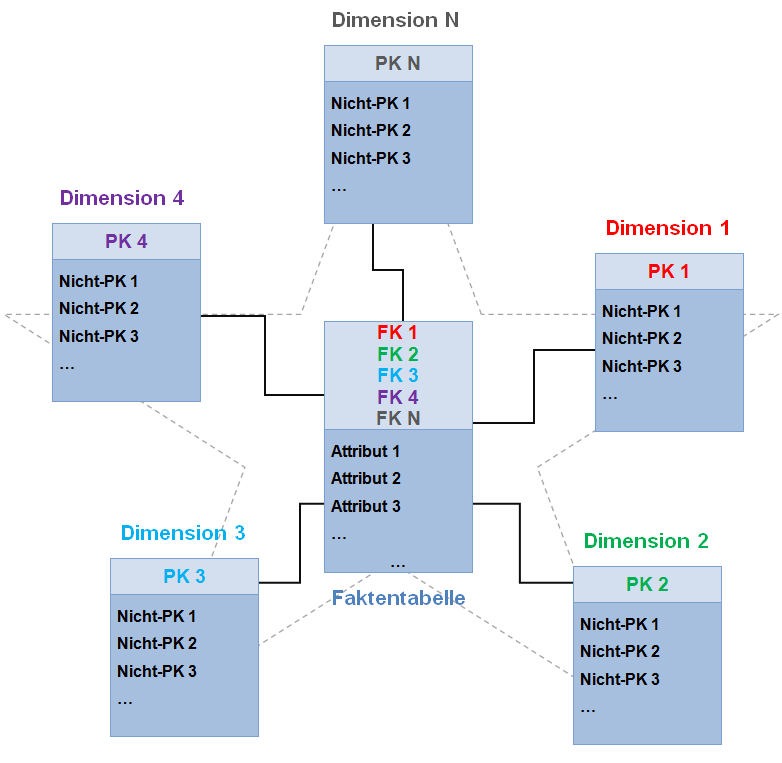
\includegraphics[scale = 0.3]{attachment/chapter_1/screenshot061}
	\caption{}
	\label{fig:screenshot061}
\end{figure}
\paragraph{Snowflake Model}
Ein \textit{snowflake model} erlaubt Beziehungen zwischen \textit{lookup tabels}. Es entsteht ein immer weiter ausbreitendes Muster.
\begin{figure}[H]
	\centering
	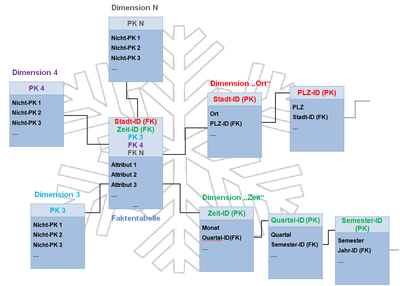
\includegraphics[scale = 0.3]{attachment/chapter_1/screenshot060}
	\caption{}
	\label{fig:screenshot060}
\end{figure}
In dem gewählten Beispiel wird \textbf{region$\_$id} in der primären Tabelle mit \textbf{region$\_$id} in der sekundären Tabelle verbunden. Eine verkettete Beziehung besteht jetzt zwischen der \textit{Transaktionsliste} und der \textit{Tabelle für Regionen}. Dies wird über \textbf{store$\_$id} geregelt.
\begin{figure}[H]
	\centering
	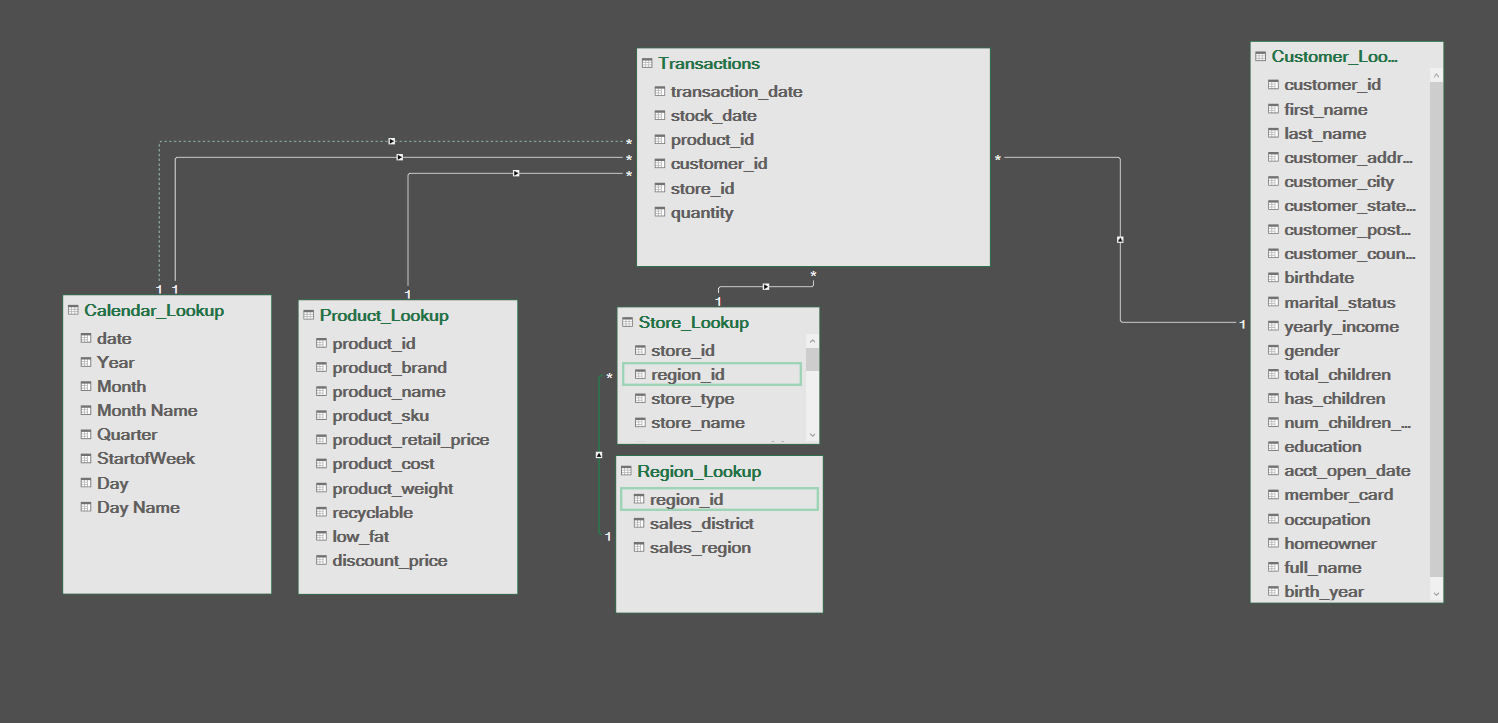
\includegraphics[scale = 0.3]{attachment/chapter_1/screenshot059}
	\caption{}
	\label{fig:screenshot059}
\end{figure}
\subsubsection{Mehrere Daten Tabellen}
Es wird stark empfohlen, zwischen \textit{LookUp} und \textit{Daten Tabellen} zu unterschieden.
Daten Tabellen werden aber nicht miteinander verbunden, sondern durch die $n:1$ Verbindung zu den jeweiligen LookUp Tabellen verbunden. Dabei wird die Pivot-Filterfunktion besser nutzbar gemacht, wie im spätern Verlauf genauer gezeigt.  
\begin{figure}[H]
	\centering
	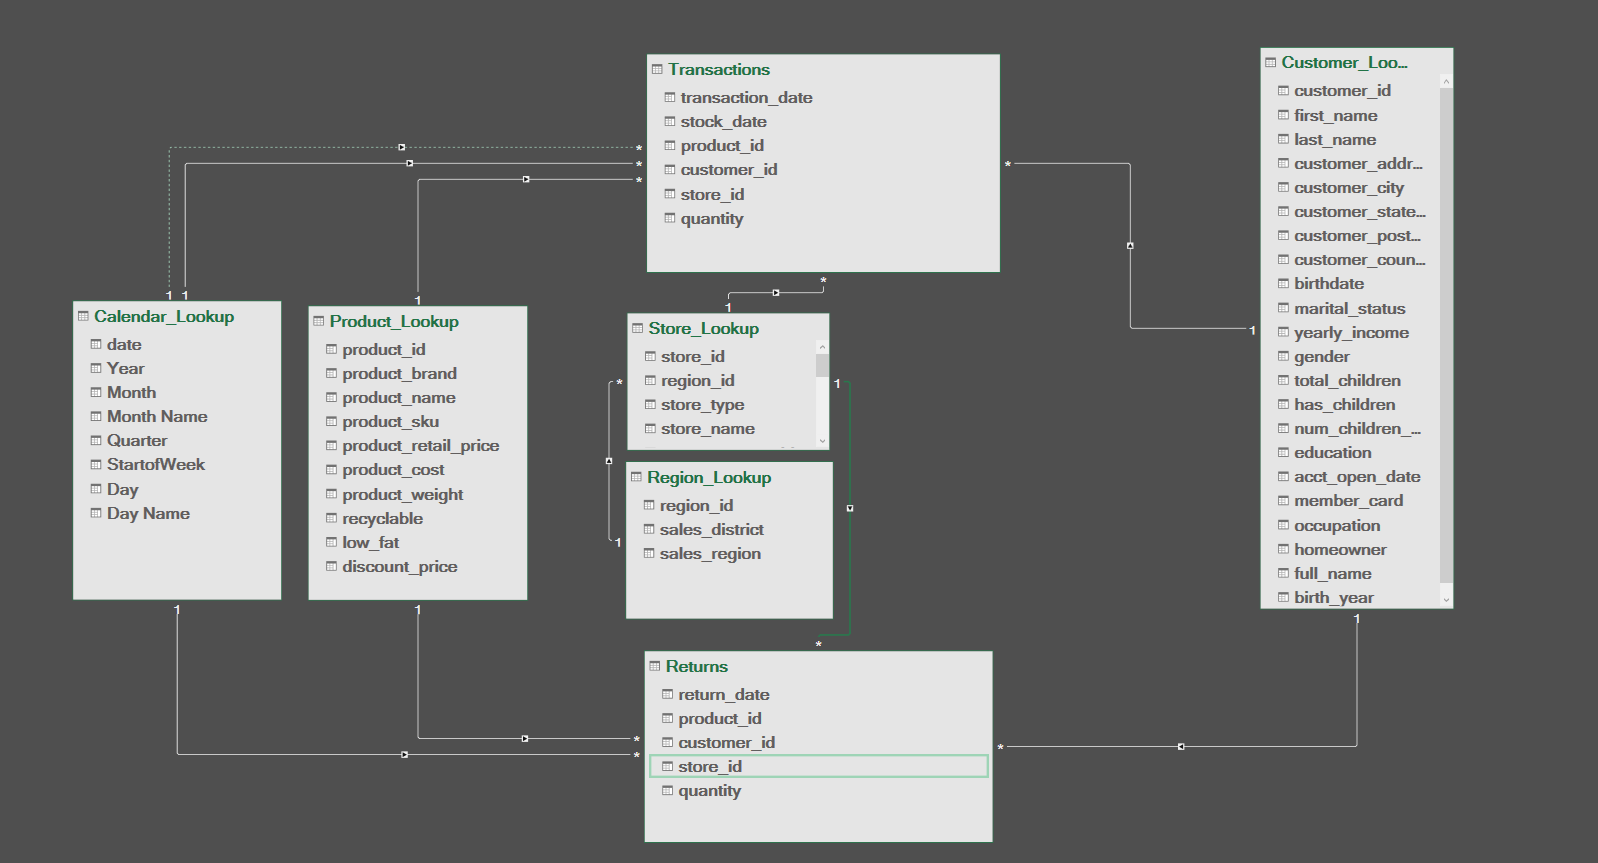
\includegraphics[scale = 0.3]{attachment/chapter_1/screenshot062}
	\caption{}
	\label{fig:screenshot062}
\end{figure}
\subsubsection{Filter}
Die Filterfunktion in den \textit{PivotTable Fields} richtet sich nach den $n:1$ Richtung. Es kann nur sinnvoll gefiltert von dem LookUp table. \textbf{Filter} $\underline{und}$ \textbf{Rows} müssen aus den LookUP Tabelle kommen! Die linke Seite kommt somit aus den Lookup Tabellen und die rechte Seite von den Daten Tabellen.
\begin{figure}[H]
	\centering
	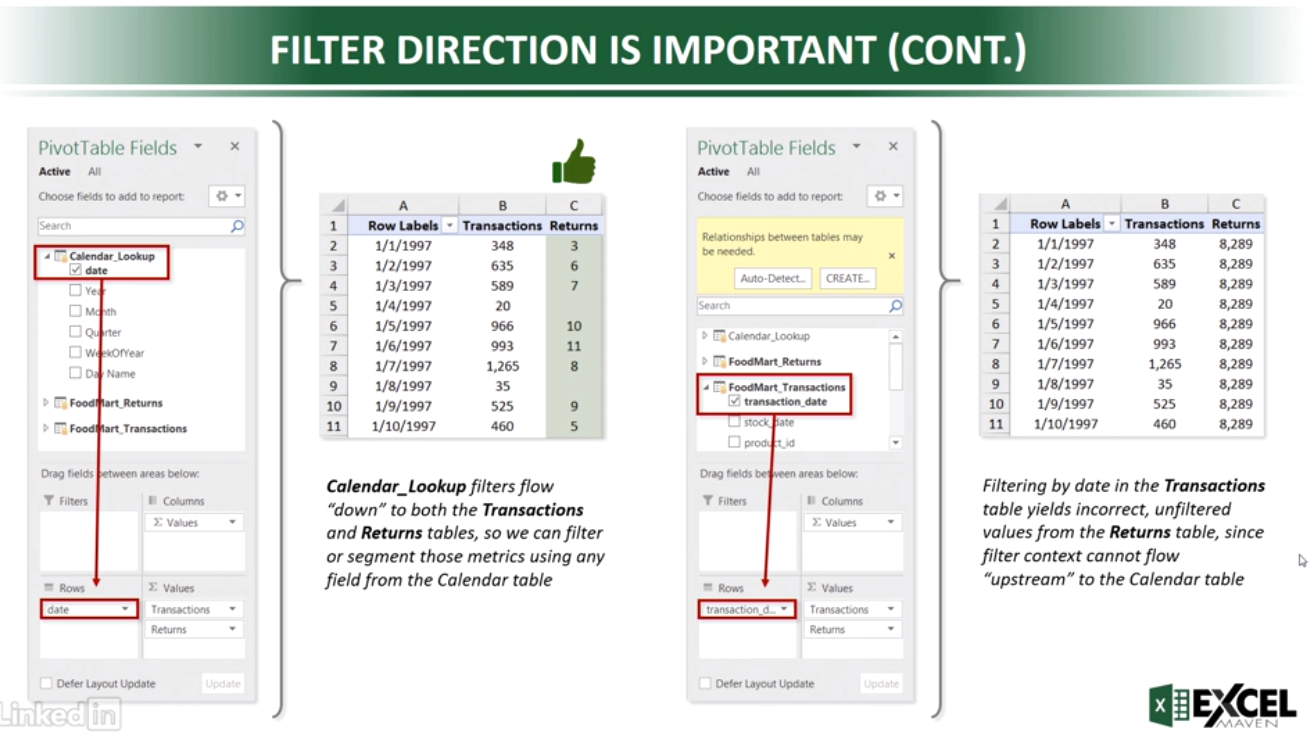
\includegraphics[scale = 0.3]{attachment/chapter_1/screenshot063}
	\caption{}
	\label{fig:screenshot063}
\end{figure}
In dem Beispiel gibt es zwei Daten Tabellen: Transaction und Return. 
Die spezifischen Werte können in die $\sum \textbf{Values}$ Spalte eingefügt werden. Die Felder für \textbf{Filter} können mit weiteren Spalten für die ID's in den Lookup Tabellen eingefügt werden. Dafür eignet sich auch ein \textit{kontinuierlicher Kalender}. Führt man die Abfrage durch Power Query durch, so kann man die aktuellen und relevantesten Daten filtern. Diese werden dann extrahiert und ein eigener Kalender mit den extrahierten unter Bewertungen kann geschaffen werden. \\
\begin{figure}[H]
	\centering
	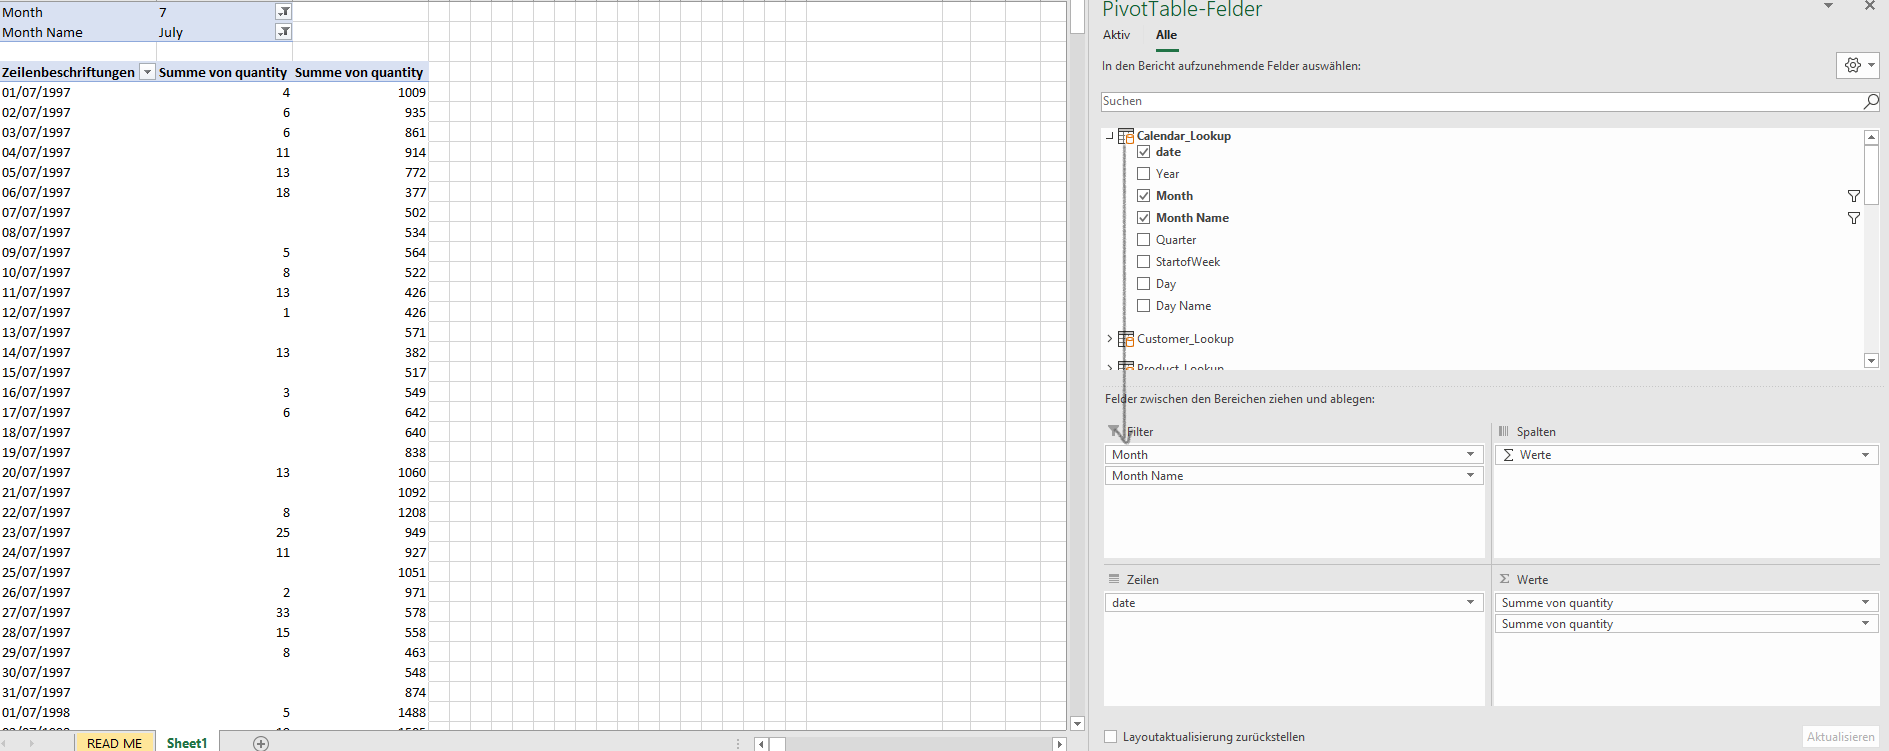
\includegraphics[scale = 0.3]{attachment/chapter_1/screenshot067}
	\caption{}
	\label{fig:screenshot067}
\end{figure}
In dem Bereich für \textbf{Spalten} und \textbf{Zeile} gilt ebenfalls, soll eine Verfeinerung der Daten aufgegriffen werden $\&$ mehrere Werte werden aus unterschiedlichen Tabellen abgegriffen, so muss die Granulierung für jeden Daten Tabelle erfolgen. Dabei muss die Spalte aus der Lookup Tabelle kommen. 
\begin{figure}[H]
	\centering
	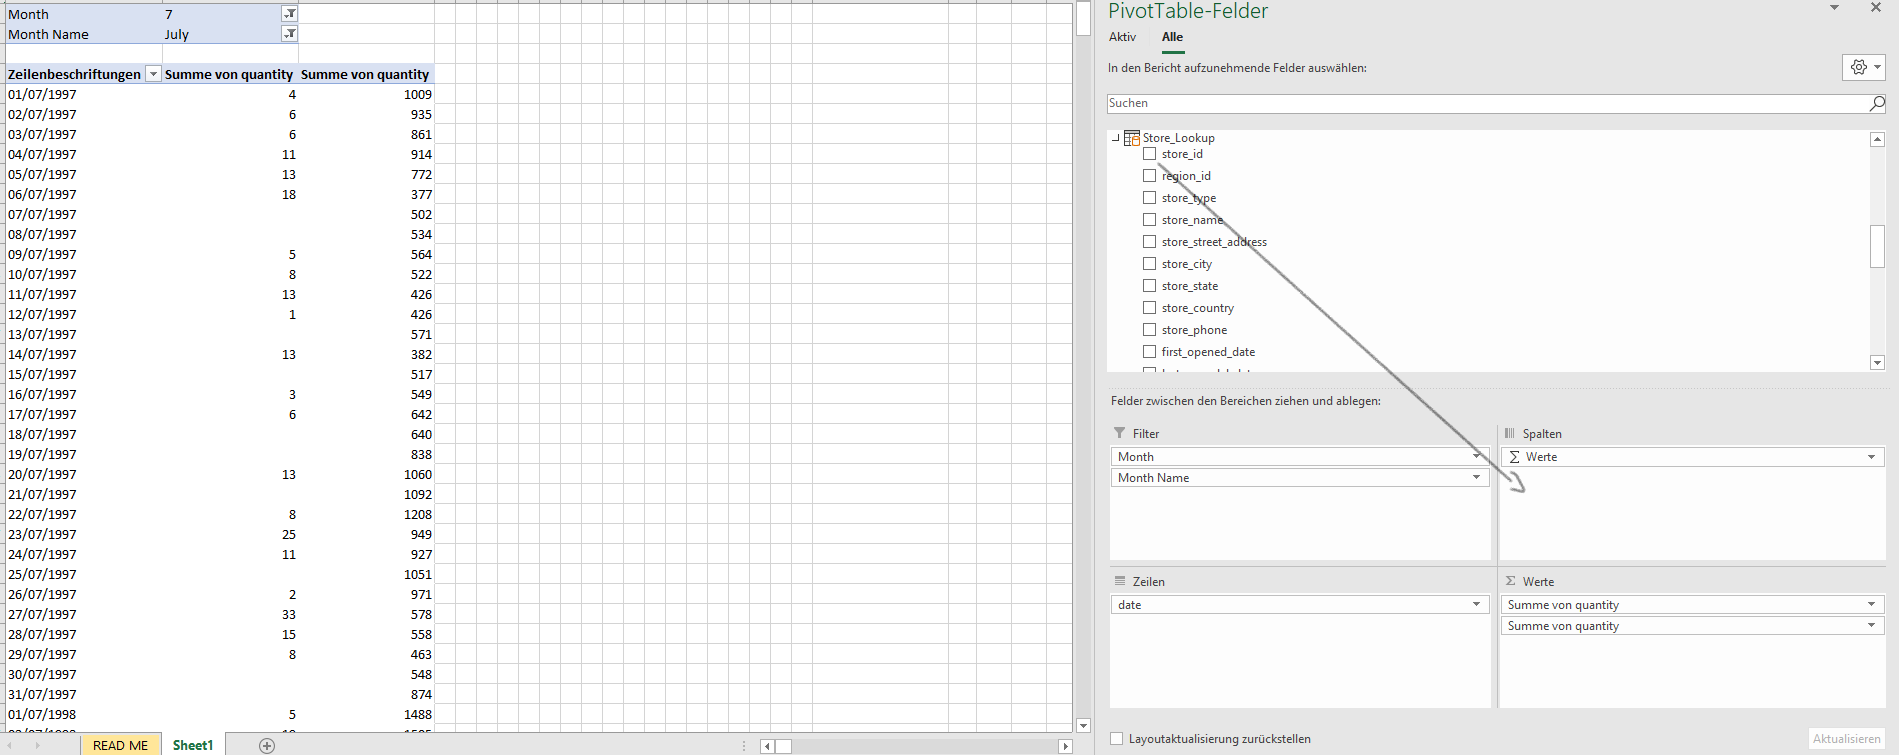
\includegraphics[scale = 0.3]{attachment/chapter_1/screenshot065}
	\caption{}
	\label{fig:screenshot065}
\end{figure}
Ein extrahieren aus einer der Daten Tabelle wird einen Fehler aufrufen, da die Filterung nicht über den Lookup Tabelle $"$durchfließt$"$. 
\subsubsection{Hide fields form client tools}
Im vorherigen Teil wurde der Fokus darauf gelegt, welche Bereich zum Filtern geeignet sind und welche nicht. Die Regel ist hier:
\begin{align}
	\text{Filter (Slice), Zeilen und Spalten enthalten \textit{Foreign Key}'s.}
\end{align}
Ein fälschlicherweise Filtern eines primären Schlüssel (Spalte) wird verhindert, indem die primären Key's in der Daten Tabelle versteckt werden. Dies geschieht nicht im Modell selber, aber im Pivot Field Bereich.\\

\begin{figure}[H]
	\centering
	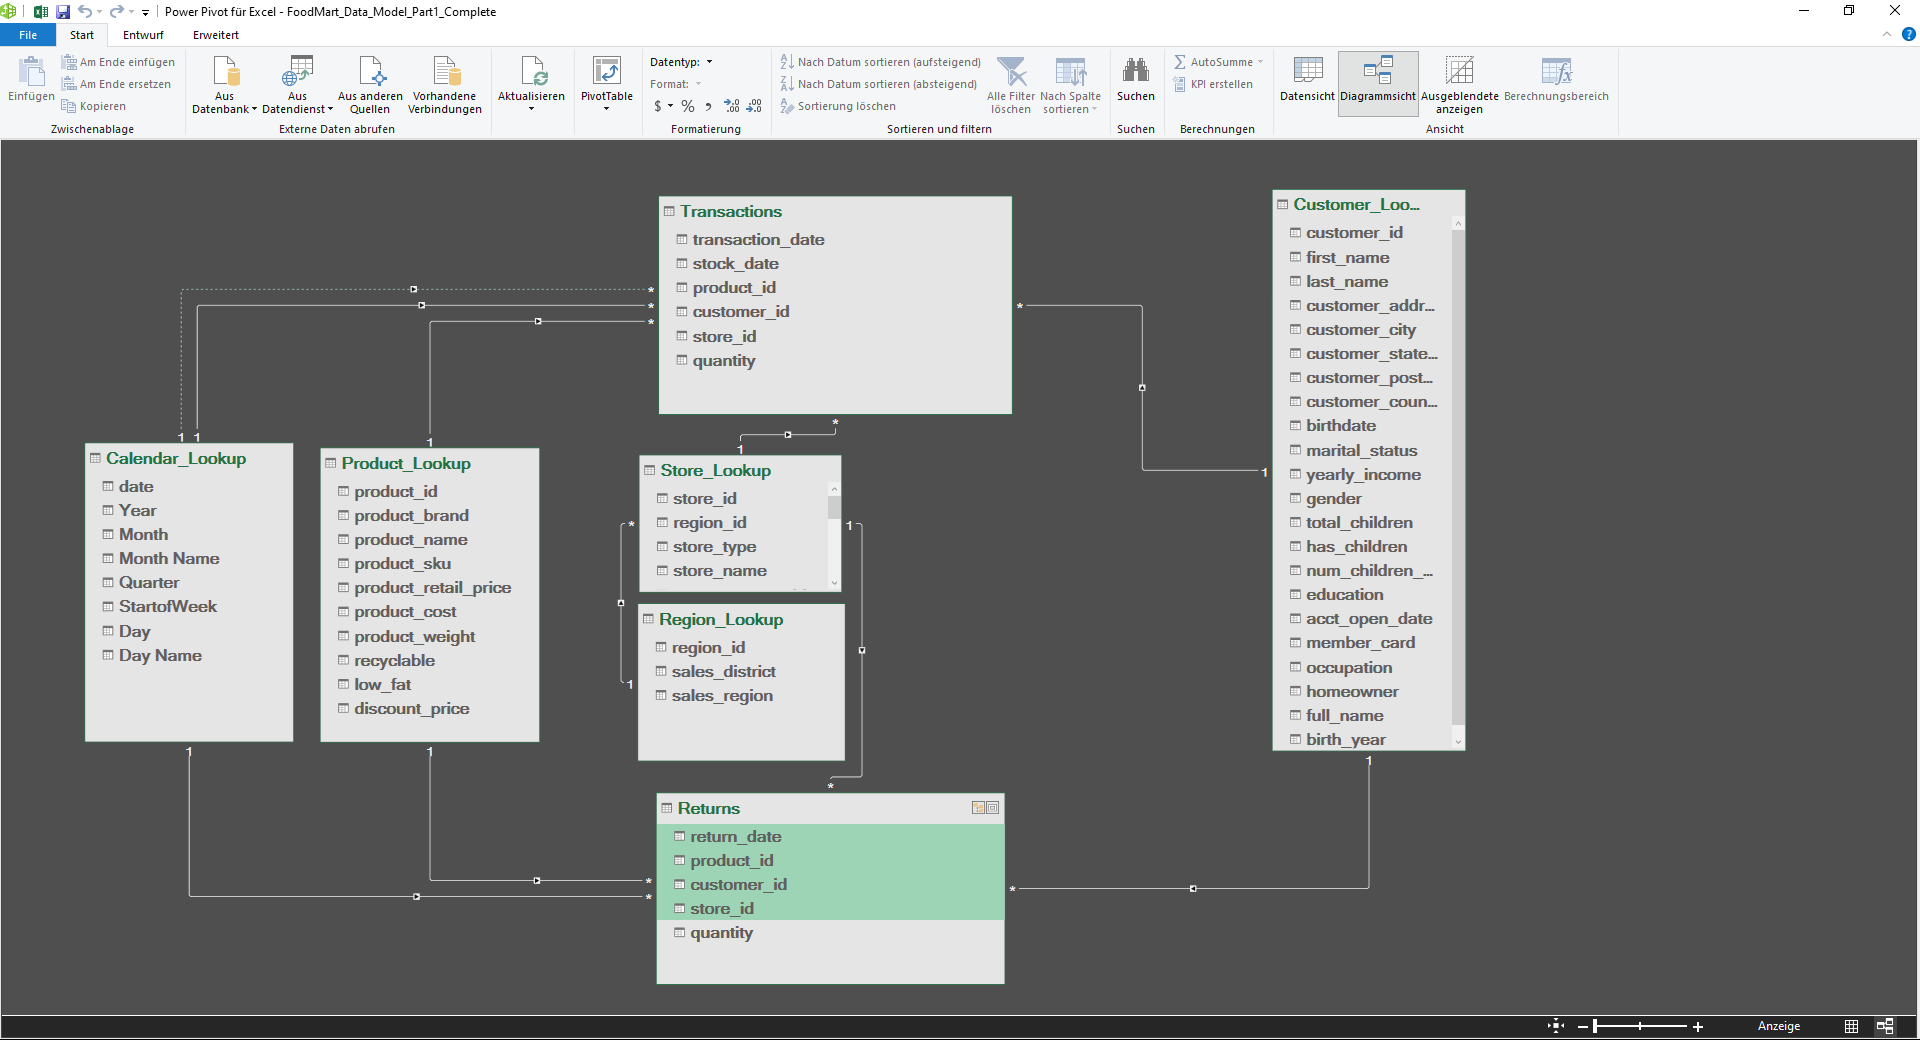
\includegraphics[scale = 0.3]{attachment/chapter_1/screenshot068}
	\caption{}
	\label{fig:screenshot068}
\end{figure}
Verwendet man die \textit{auszublendenden Funktion}, werden die Key's nicht mehr angezeigt. 
\begin{figure}[H]
	\centering
	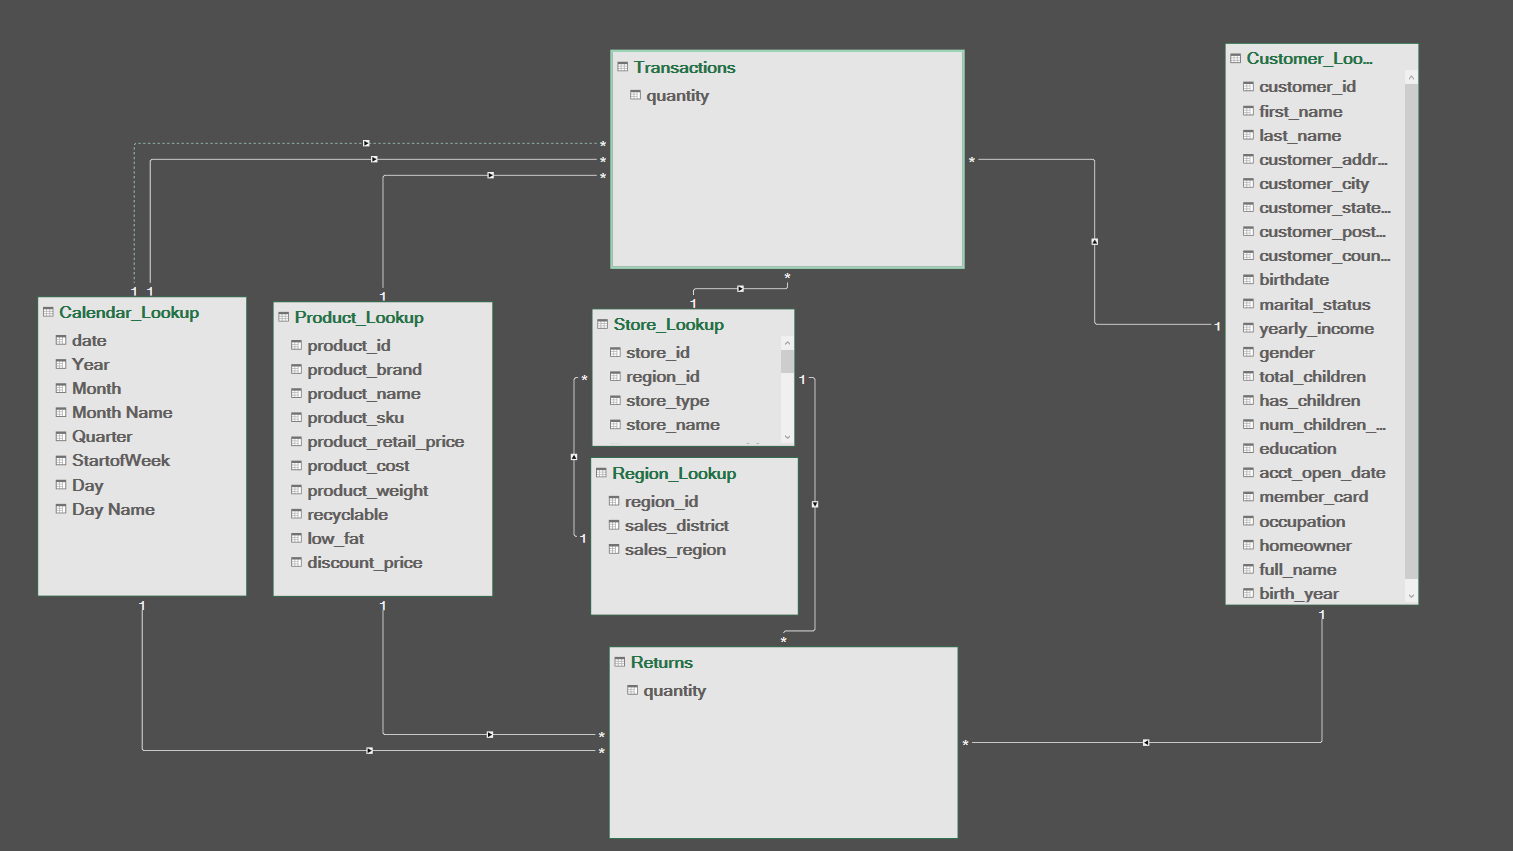
\includegraphics[scale = 0.3]{attachment/chapter_1/screenshot069}
	\caption{}
	\label{fig:screenshot069}
\end{figure}
Mit der Funktion an, wenden die Key's grau Schraffiert markiert.
\begin{figure}[H]
	\centering
	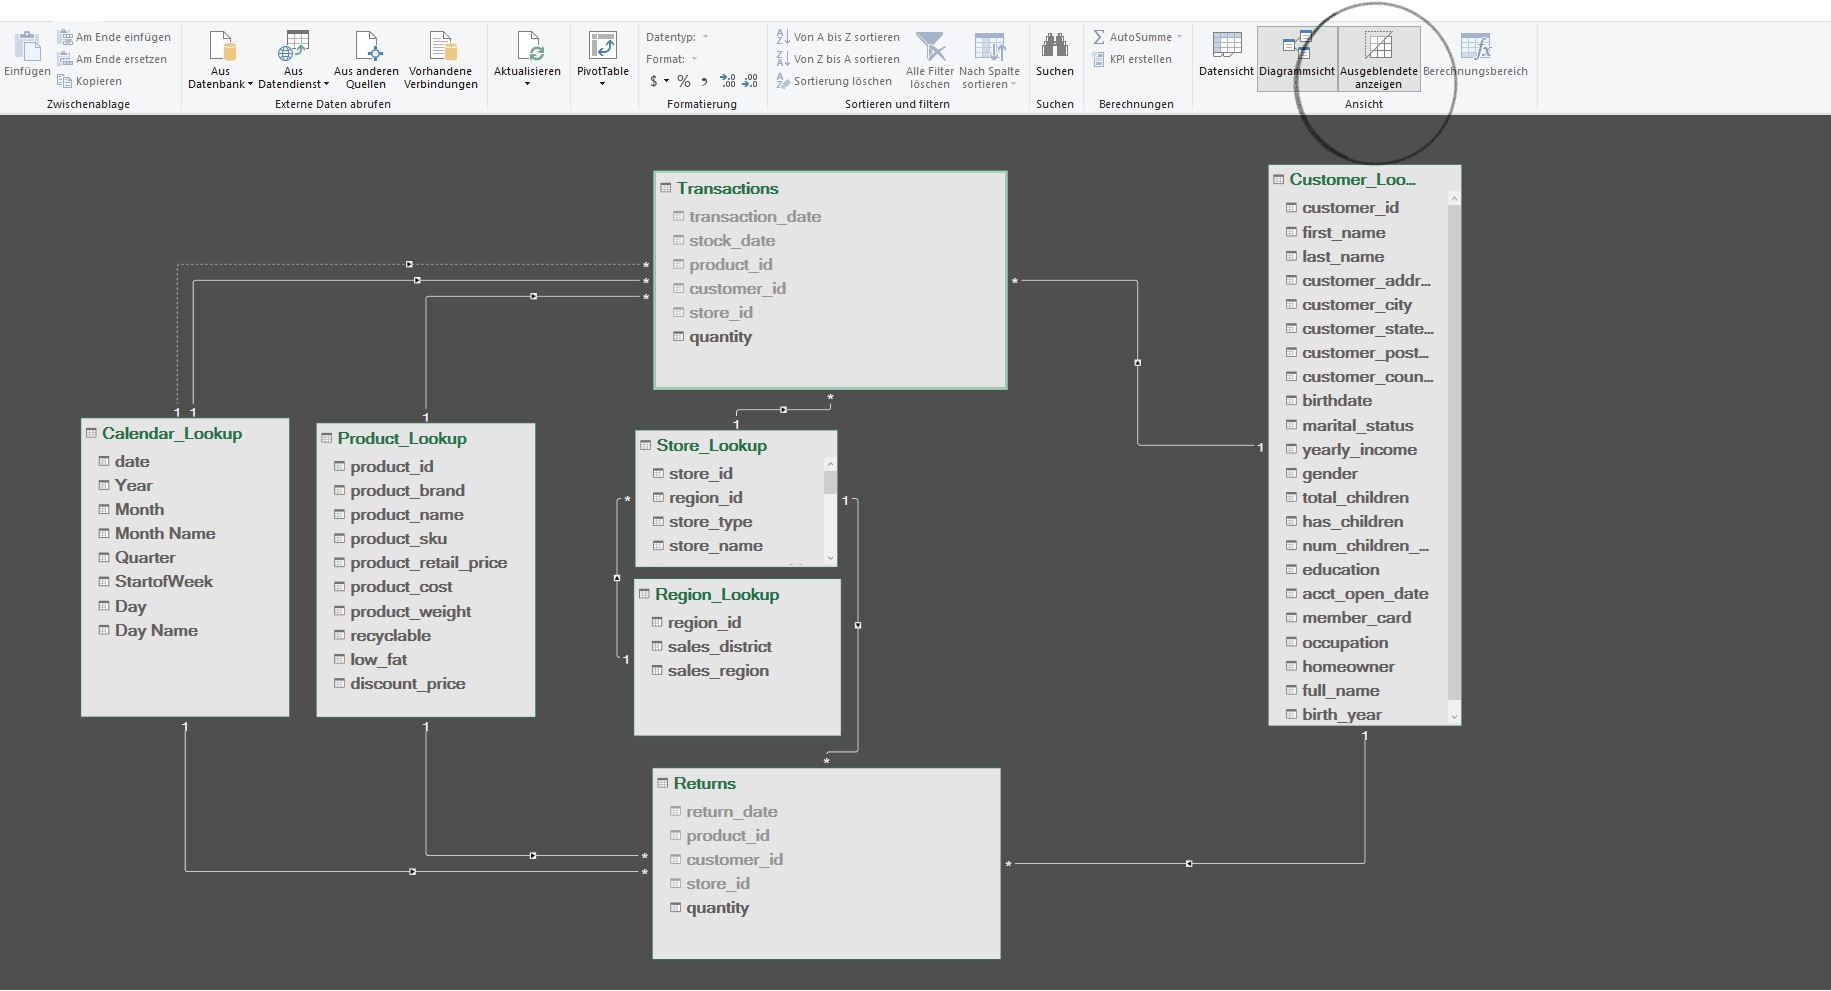
\includegraphics[scale = 0.3]{attachment/chapter_1/screenshot070}
	\caption{}
	\label{fig:screenshot070}
\end{figure}
\subsubsection{Hierarchy}
Mit Hilfe der Hierarchy können Gruppierungen von Foreign Key's erstellt werden, welche Inhaltlich zu sammenpassen. Dabei ist die Zeit eine naheliegende Tabelle.
\begin{figure}[H]
	\centering
	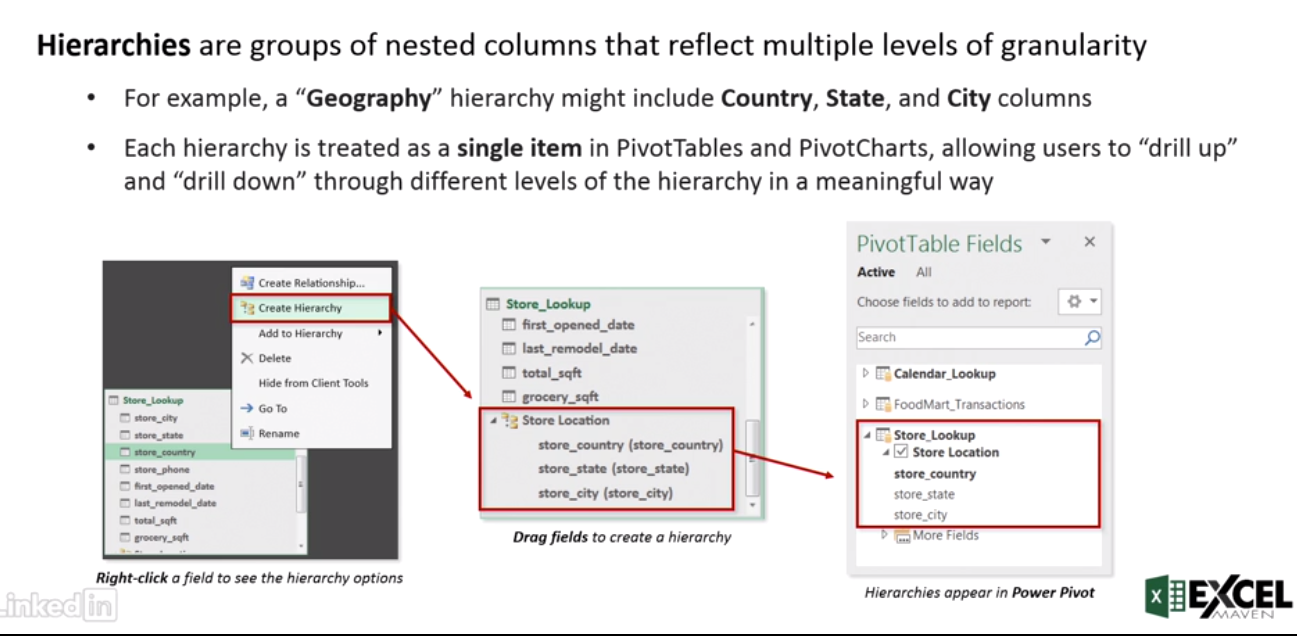
\includegraphics[scale = 0.3]{attachment/chapter_1/screenshot071}
	\caption{}
	\label{fig:screenshot071}
\end{figure}
Den Effekt wird im dritten Teil des Dreiteilers besprochen.
\begin{figure}[H]
	\centering
	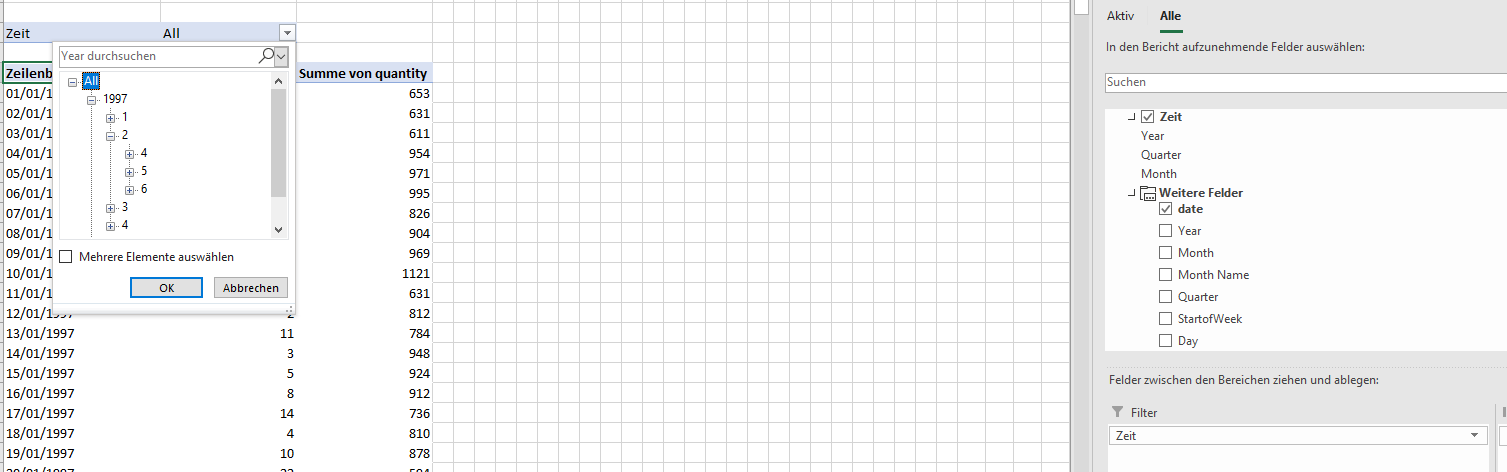
\includegraphics[scale = 0.3]{attachment/chapter_1/screenshot072}
	\caption{}
	\label{fig:screenshot072}
\end{figure}
\section{Business Intelligence: Power Pivot and DAX}
\subsection{Power Pivot 101}
\subsubsection{Oberfläche von Power Pivot}
Einige Objekte der Oberfläche wurden schon in den vorherigen Kursen behandelt. Die Resultate können am Ende der Prozesses per \textit{Pivot Tabelle} Schaltfläche in Excel eingeführt werden. 
\begin{figure}[H]
	\centering
	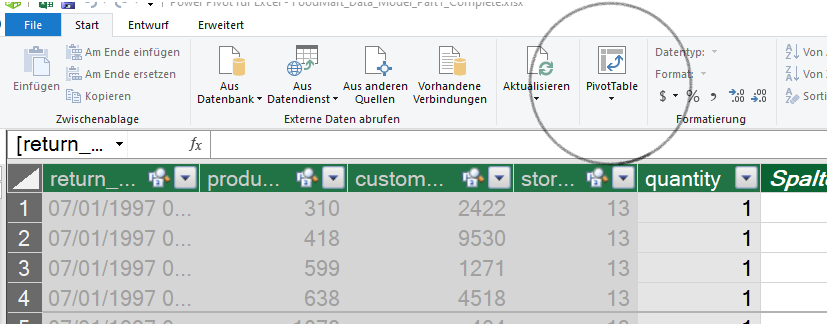
\includegraphics[scale = 0.3]{attachment/chapter_1/screenshot073}
	\caption{}
	\label{fig:screenshot073}
\end{figure}
Über diese Funktion können verschiedenen Kombinationen von Pivot Tabellen und Grafiken eingefügt werden. 
\subsubsection{Berechnungen}
\subsubsection{Funktion mit normalen Tabellen}
Tabellen die nicht über das Datenmodell verarbeitet sind und direkt mit Power Pivot eingefügt werden können die die \textbf{Berechnete Feld} Funktion nicht nutzten. Diese sind ausgegraut.
\begin{figure}[H]
	\centering
	\includegraphics[scale = 0.3]{attachment/chapter_1/screenshot074}
	\caption{}
	\label{fig:screenshot074}
\end{figure}
Tabellen die nicht im Daten Modell liegen, können extra Felder zu der Tabelle hinzufügen ohnen an den \textit{Rohdaten} etwas zu verändern. 
\begin{figure}[H]
	\centering
	\includegraphics[scale = 0.3]{attachment/chapter_1/screenshot075}
	\caption{Öffnen}
	\label{fig:screenshot075}
\end{figure}
\begin{figure}[H]
	\centering
	\includegraphics[scale = 0.3]{attachment/chapter_1/screenshot076}
	\caption{$f(x)= $2 mal Menge}
	\label{fig:screenshot076}
\end{figure}

\subsubsection{Calculated Columns}
Berechnende Spalten sind ähnlich aufgebaut, wie erweiternden Spalten in Tabellen. Es ist ratsam, diese gleich über Power Query anzulegen. Diese werden meist verwendet, um Slicer, Zeilen oder Spalten Granulierungen vorzunehmen. 
\begin{figure}[H]
	\centering
	\includegraphics[scale = 0.3]{attachment/chapter_1/screenshot077}
	\caption{}
	\label{fig:screenshot07}
\end{figure}
Die benutzerdefinierten Spalten werden für einzelnen Tabellen verwendet. Die \textbf{Measures} werden für das gesamte Datenmodell verwendet. Alles was mit aggregierten Werten zu tun hat, wird darüber bestimmt. 
\begin{figure}[H]
	\centering
	\includegraphics[scale = 0.3]{attachment/chapter_1/screenshot078}
	\caption{}
	\label{fig:screenshot078}
\end{figure}
Ebenso ist zu berücksichtigen, dass es aggregierte Werte geben kann, diese werden dann aber für jeden Zeile verwendet.
\begin{figure}[H]
	\centering
	\includegraphics[scale = 0.3]{attachment/chapter_1/screenshot079}
	\caption{}
	\label{fig:screenshot079}
\end{figure}
Einig der \gls{DAX} Funktion sind gleich von der Syntax und dein Eingabewerten wie in Excel.
\begin{figure}[H]
	\centering
	\includegraphics[scale = 0.3]{attachment/chapter_1/screenshot080}
	\caption{}
	\label{fig:screenshot080}
\end{figure}
\subsubsection{Implicit Funktionen}
Zieht man die Spalten von den Daten Tabellen in den \textit{Werte Bereich} wir die Auswahl von verschiedenen Funktionen geben. Diese Funktionen nennt man \textbf{Implicit Function}.
\begin{figure}[H]
	\centering
	\includegraphics[scale = 0.3]{attachment/chapter_1/screenshot081}
	\caption{}
	\label{fig:screenshot081}
\end{figure}
Die Funktionen sind fix vorgegeben. Warum oft darauf hingewissen ist, \textit{explicit function} zu nutzen, liegt daran, dass implizierte Funktionen fix und keine weiteren Änderungen an ihnen vorgenommen werden kann. 
\begin{itemize}
\item Der Name der Funktion kann nicht verändert werden.  
\item Zahlenformate zu den Funktionen kann nicht geändert werden. Hinweis: Soll ein gewisses Zahlenformat beibehalten werden, bietet Power Pivot explizite Funktionen an, das Format fix zu halten. Dabei wird bei jeder weiteren Verwendung der Funktion das Dateiformat angepasst.
\end{itemize}

\subsubsection{Explicit Funktionen - Measures}
Einfache \textbf{expliziete Funktionen} werden in die Tabellen in Funktionsbereich geschrieben. 
\begin{figure}[H]
	\centering
	\includegraphics[scale = 0.3]{attachment/chapter_1/screenshot082}
	\caption{}
	\label{fig:screenshot082}
\end{figure}
Bildet man die gleiche implizierte Funktion nach, so funktioniert sie auch in gleicher Weise.
\begin{figure}[H]
	\centering
	\includegraphics[scale = 0.3]{attachment/chapter_1/screenshot083}
	\caption{}
	\label{fig:screenshot083}
\end{figure}
Die Verwaltung der \textit{expliziten Funktionen} kann auch über Excel unter \textit{Power Pivot/ Measures} eingesehen werden.
\begin{figure}[H]
	\centering
	\includegraphics[scale = 0.3]{attachment/chapter_1/screenshot084}
	\caption{}
	\label{fig:screenshot084}
\end{figure}
Wir ein \textit{Measures} erstellt, kann dies ebenfalls über das Eingabefeld erfolgen.
\begin{figure}[H]
	\centering
	\includegraphics[scale = 0.3]{attachment/chapter_1/screenshot085}
	\caption{}
	\label{fig:screenshot085}
\end{figure}
Die Zuweisung hat nicht damit zu tun, dass nur Werte aus der Tabelle verwendet werden können, sondern damit zu welcher Tabelle es im Pivot Field angezeigt wird. 
Die \textit{expliziten Funktionen} werden deshalb bevorzugt, weil
\begin{itemize}
\item eine genau Bezeichnung möglich ist.
\item Measures aus verschiedenen Tabellen zusammengeführt werden könnnen.
\item Datentypen angepasst werden können.
\end{itemize} 

\begin{figure}[H]
	\centering
	\includegraphics[scale = 0.3]{attachment/chapter_1/screenshot086}
	\caption{}
	\label{fig:screenshot086}
\end{figure}

\subsubsection{Filterfunktion}
Die Art und Weise wie Filter (Slicer), Zeilen und Spalten verwendet werden können, kann als Wasserfall-Diagramm verstanden werden. Die Filter werden in den Lookup Tabellen gesetzt. Über die Key's werden die Tabellen, welche in Beziehung zu der Lookup Tabelle stehen gefiltert. Soll ein Filter für mehrere Daten Tabellen angelegt werden, wo werden nämlich alle Tabellen gefiltert, welche in Beziehung stehen. Ein lokaler Slicer kann im Zweifelsfall über eine eigene Spalte in der Datentabelle erstellt werden. Die Filterfunktion erstreckt sich dabei über alle Spalten, die in der Lookup Tabelle zu finden sind, selbst wenn sie in der ursprünglichen Tabelle nicht angefügt wurden.\\

Erzeugte Slicer müssen mit anderen Verweisen verbunden werden, sodass die Daten upgedatet werden sollen. Sonst bleiben auch verknüpfte Koordinaten-Kategorien seperat.
\subsection{Basic DAX Function}
\subsubsection{Syntax und Operatoren}
Die \gls{DAX} Sprache ist eine Funktionssprache. Dies bedeutet, ein \gls{g_Measure} muss eine Funktion enthalten, die eine Form der Aggregations zu lässt. Hingegen können \gls{g_Berechnende-Spalte} ohne Funktionen auskommen und einfache Operatoren verwenden. \\
Die gängigsten Operatoren für \gls{DAX} sind:

\begin{figure}[H]
	\centering
	\includegraphics[scale = 0.3]{attachment/chapter_1/screenshot087}
	\caption{}
	\label{fig:screenshot087}
\end{figure}
Für \textit{and} wird $\&\&$ verwendet, und für \textit{or} werden zwei vertikale Trennstriche verwendet. 
Für die Syntax der Funktionen kann Power Query verwandt werden. Die Referenz zu einer Spalte in einer Tabelle funktioniert gleich. Variablen Namen werden aber anders gehandhabt. Namen mit Leerzeichen werden mit einfachen Anführungsstrichen umschloßen.
\begin{figure}[H]
	\centering
	\includegraphics[scale = 0.3]{attachment/chapter_1/screenshot088}
	\caption{}
	\label{fig:screenshot088}
\end{figure}
Die Funktionen ähneln den die aus Excel und Power Query bekannt sind. Im weiteren Verlauf wird aber noch verstärkt auf einzelne Funktionen eingegangen.

\begin{figure}[H]
	\centering
	\includegraphics[scale = 0.3]{attachment/chapter_1/screenshot089}
	\caption{}
	\label{fig:screenshot089}
\end{figure}

\subsubsection{Function} 
Für numberische Werte können viele verschiedenen Spalten hinzugefügt werden.

\begin{figure}[H]
	\centering
	\includegraphics[scale = 0.3]{attachment/chapter_1/screenshot090}
	\caption{}
	\label{fig:screenshot090}
\end{figure} 

Werden mehrer Spalten hinzugefügt, so können Sortierungen über die Zeilenfilterung durchgeführt werden.


\begin{figure}[H]
	\centering
	\includegraphics[scale = 0.3]{attachment/chapter_1/screenshot091}
	\caption{}
	\label{fig:screenshot091}
\end{figure} 

\begin{figure}[H]
	\centering
	\includegraphics[scale = 0.3]{attachment/chapter_1/screenshot092}
	\caption{}
	\label{fig:screenshot092}
\end{figure}
Einfache Logische Funktionen verhalten sich wie schon oben beschrieben. Bei \textit{And()} und \textit{Or()} Funktionen können auch mit den dazugehörigen Operatoren beschrieben werden. Sollen mehrere Menge zusammengefasst werden, nimmt man die Operatoren.
\begin{figure}[H]
	\centering
	\includegraphics[scale = 0.3]{attachment/chapter_1/screenshot092}
	\caption{}
	\label{fig:screenshot092}
\end{figure} 
\paragraph{Switch Function}
Ein einfacher Austausch von Werten.
\begin{figure}[H]
	\centering
	\includegraphics[scale = 0.3]{attachment/chapter_1/screenshot094}
	\caption{}
	\label{fig:screenshot094}
\end{figure}
Switch erlaubt auch eine Variante, in der mehrer Überprüfungen vorgenommen werden können. In der ersten Übergabe wird $true()$ übergeben.
\paragraph{Text Funktionen} 

\begin{figure}[H]
	\centering
	\includegraphics[scale = 0.3]{attachment/chapter_1/screenshot095}
	\caption{}
	\label{fig:screenshot095}
\end{figure}
\subsection{Advanced DAX Function}
Die bisherigen Funktionen finden sich ein der einen oder anderen Form in Excel oder auch der M-Query Sprache wieder. Es gibt aber auch komplexerer Funktion in \gls{DAX}. Die $Calculate$ Funktion. Diese erlaubt komplizierte Berechnungen, basierend an verschiedenen Filtern. Dies ist nützlich, wenn Berechnungen nur für bestimmte Felder ausgeführt werden sollen. 
\begin{figure}[H]
	\centering
	\includegraphics[scale = 0.3]{attachment/chapter_1/screenshot096}
	\caption{}
	\label{fig:screenshot096}
\end{figure} 
\subsubsection{Calculate} 
Dies Funktion nimmt in als erstes Argument eine Variable vom Typ table auf. Als zweites Argument wird ein Filter eingesetzte. Dabei wird die Tabelle, Stream up, gefiltert. Dieser Filter wird dann weiter gegeben und die Berechnungen im ersten übergebenen Tabelle oder Tabellen berechnet. Es ist eine verbesserte Variante der \textit{Sumif}-Funktion. Die Funktionsweise für \gls{DAX} Funktionen ist aber wichtig zu verstehen. Die Filter in der dazugehörigen Tabellen werden aktiviert und diese Filter werden für das Measure komplett im Datenmodell weitergeben. Die Berechnungen mit $n$-Tabellenspalten im ersten Bereich werden dann durchgeführt, unter Berücksichitung der Filter. \\
Wie man sieht werden vorherige, übergebene Filter überschrieben, weswegen in jeder Zeile der gleiche Wert steht.
\begin{figure}[H]
	\centering
	\includegraphics[scale = 0.3]{attachment/chapter_1/screenshot097}
	\caption{}
	\label{fig:screenshot097}
\end{figure} 


Der Filter, als zweites Argument, kann auch eine Tabelle enthalten. 
In diesem Fall wird die Tabelle, die gefiltert wird, ersetzt und die Tabelle, welche durch die Filter-Funktion gefiltert wurde, ersetzt temporär die angegebene Tabelle. 
\begin{figure}[H]
	\centering
	\includegraphics[scale = 0.3]{attachment/chapter_1/screenshot098}
	\caption{}
	\label{fig:screenshot098}
\end{figure} 
Mit der Filter-Funktion existieren die gesuchten Filter nicht mehr und die Zeilen bleiben gleich.

\begin{figure}[H]
	\centering
	\includegraphics[scale = 0.3]{attachment/chapter_1/screenshot099}
	\caption{}
	\label{fig:screenshot099}
\end{figure} 

\subsubsection{Filter}
Die Filterfunktion erhält als Input eine Tabelle. Die Filterfunktion wird mit Angaben von Spezifikation von Spalten erstellt. Der Funktion gibt eine Tabelle wieder.

\begin{figure}[H]
	\centering
	\includegraphics[scale = 0.3]{attachment/chapter_1/screenshot100}
	\caption{}
	\label{fig:screenshot100}
\end{figure} 


Wie kann man \textbf{Ergänzende-Slicer} in eine ein Datenmodell einfügen, ohne es mit den restlichen Tabellen zu verbinden $\rightarrow$ mit der Filterfunktion. Die Tabelle Der Filter in der Filterfunktion kann durch eine extra-eingefügte Tabelle gebunden werden. \\ 

1. Die MAX-Funktion gibt nur einen Wert wieder:

\begin{figure}[H]
	\centering
	\includegraphics[scale = 0.3]{attachment/chapter_1/screenshot102}
	\caption{}
	\label{fig:screenshot102}
\end{figure} 

Die Einbindung läuft über zwei \gls{g_Measure}.

\begin{figure}[H]
	\centering
	\includegraphics[scale = 0.3]{attachment/chapter_1/screenshot101}
	\caption{}
	\label{fig:screenshot101}
\end{figure} 
Hinweis: Dies Funktion wäre auch sinnvoll, wenn es um die Prämienberechnung geht. In dem man die einzelnen \textbf{Threshold} angibt. 
Zusätzlich, es können auch Slicer direkt über die Ansicht der Pivot-Tabellen angezeigt werden.

\begin{figure}[H]
	\centering
	\includegraphics[scale = 0.3]{attachment/chapter_1/screenshot103}
	\caption{}
	\label{fig:screenshot103}
\end{figure} 

\subsubsection{All}
Die All-Funktion ignoriert die bisher angewendeten Filter zu einer Tabelle. Dies erlaubt Berechnungen vorzunehmen, welche nicht nicht ändern sollen, wenn interaktiv Filter angewandt werden.

\begin{figure}[H]
	\centering
	\includegraphics[scale = 0.3]{attachment/chapter_1/screenshot104}
	\caption{}
	\label{fig:screenshot104}
\end{figure} 

Angenommen, es ist verlangt, eine Tabelle mit prozentualen Verhältnissen zu zeigen. \begin{figure}[H]
	\centering
	\includegraphics[scale = 0.3]{attachment/chapter_1/screenshot105}
	\caption{}
	\label{fig:screenshot105}
\end{figure} 
Dies ist nur möglich, wenn die Summe am Ende gleich bleibt, wenn man möchte, dass durch Selektion die Prozente sich nicht verändern. Die All-Funktion erlaubt, die Verhältnise bei zu behalten, selbst wenn die Zeilen gefiltert werden.
Zum Beispiel könnte das Measures heißen:
\begin{align}
Statis_Prozent_=\frac{[Transaction]}{Sum(All([Transaction]))} 
\end{align} 
\subsubsection{Iterator (X) - SumX()}
Das Grundprinzip von \gls{g_Measure} ist, dass die Funktion einen Wert und keine Tabelle oder Spalte wieder gibt. Eine Aggregation von Text ist somit im einzelnen nicht möglich, außer, eine klevere Funktion wird geschrieben. \\
\textit{Die Steuerung wird über die Filter gesteuert!}

Die Iteratorfunktionen sind nur erweiterte Funktionen ihrer zugrundeliegenden, einfachen Funktionen. Als Beispiel, die $Sum()$ Funktion kann nur ein Aggregat einer Spalte sein. 

\begin{figure}[H]
	\centering
	\includegraphics[scale = 0.3]{attachment/chapter_1/screenshot106}
	\caption{}
	\label{fig:screenshot106}
\end{figure} 
Dabei wird erst die komplette erste Spalte und danach die komplette zweite Spalte aggregiert. Erst dann, werden die beiden Skalare miteinander multipliziert. Bei der Iterator Funktion wird, wird Zeile für Zeile summiert und im Anschluss aggregiert. Dies macht auch die $Calculate()$ Funktion. Dabei wird nur zusätzlich ein Filter benötigt. 

\begin{figure}[H]
	\centering
	\includegraphics[scale = 0.3]{attachment/chapter_1/screenshot107}
	\caption{}
	\label{fig:screenshot107}
\end{figure} 

Die $SumX()$ Funktion verlangt eine Tabelle, von welcher die Berechnungen ausgehen. Es kann aber mit der $Related()$ Funktion Daten aus anderen Tabellen gezogen werden. 

\begin{figure}[H]
	\centering
	\includegraphics[scale = 0.3]{attachment/chapter_1/screenshot108}
	\caption{}
	\label{fig:screenshot108}
\end{figure} 

\subsubsection{Iterator (X)- RankX()}
Die $RankX()$ Funktion ist eine iterative Funktion, weil sie erst die komplette Spalte durchlaufen muss, bevor jeder Wert in Reihe gebracht werden. 
Die Funktion gibt eine Liste von Zahlen wieder. Diese gibt an. 

\begin{figure}[H]
	\centering
	\includegraphics[scale = 0.3]{attachment/chapter_1/screenshot111}
	\caption{}
	\label{fig:screenshot111}
\end{figure} 
Es ist dabei wichtig, zu berücksichtigen, dass die Filterfunktion einen Einfluss auf die Funktion hat. Die Funktion $All()$ erlaubt, die Filter auszublocken und einen Ordnung der Werte zu ermöglichen, obwohl sie gefiltert sind.

\begin{figure}[H]
	\centering
	\includegraphics[scale = 0.3]{attachment/chapter_1/screenshot110}
	\caption{}
	\label{fig:screenshot110}
\end{figure} 
Weitere Unterteilungen kann wie folgt aussehen.

\begin{figure}[H]
	\centering
	\includegraphics[scale = 0.3]{attachment/chapter_1/screenshot109}
	\caption{}
	\label{fig:screenshot109}
\end{figure} 

\subsubsection{Time-Intelligence Function}
Dies Funktionen verhalten sich ähnlich zu denen in $M$. 

\begin{figure}[H]
	\centering
	\includegraphics[scale = 0.3]{attachment/chapter_1/screenshot112}
	\caption{}
	\label{fig:screenshot112}
\end{figure} 

Die erste Funktion erlaubt in Abschnitten zu untergliedern. Dabei wird ein spezifischer Filter für das Datum verwandt. 
Nachdem die ersten Funktionen geschrieben sind, können die Funktionen einfach miteinander kombiniert werden. Die Funktion $DateAdd()$ erlaubt:

\begin{figure}[H]
	\centering
	\includegraphics[scale = 0.3]{attachment/chapter_1/screenshot114}
	\caption{}
	\label{fig:screenshot114}
\end{figure} 
Setzt man die Funktion ohne mit mit ins Verhältnis, so ergibt sich:

\begin{figure}[H]
	\centering
	\includegraphics[scale = 0.3]{attachment/chapter_1/screenshot113}
	\caption{}
	\label{fig:screenshot113}
\end{figure} 
Gleiches gilt auch für die Funktion für Perioden $Dateinperiode()$. Eine fixes Zeitspanne kann somit erstellt werden. 

\section{Power BI Dataflow Essentials}
Dashboard werden über Power BI Desktop erstellt. In der hochgeladenen Datei (Power BI Desktop File) befinden sich zwei Komponenten
\begin{itemize}
	\item Front End Dashboard
	\item Dataset
\end{itemize}

\subsection{Gateways and Gatway Clusters}
Um Daten einer Organisation mit der BI Cloud zu verbinden, benötigt es \textbf{On-Premise Gateways}. Diese werden auf den Server einer Organisation verbunden. Diese geben einen Zugang zum System. Die Daten müssen nicht auf der Recheneinheit liegen, auf welcher das Gatway installiert ist.
\begin{figure}[H]
	\centering
	\includegraphics[scale = 0.3]{attachment/chapter_1/Scc128}
\end{figure}
Im AdminCenter wird festgelegt, wer in der Organisation Gatways installieren kann.
Die Einschränkung kann sogar aufgehoben werden, und alle User in einer Organisation können Gatways anlegen.

\begin{figure}[H]
	\centering
	\includegraphics[scale = 0.3]{attachment/chapter_1/Scc129}
\end{figure}
Die Funktionalität \gls{AD} Group hinzuzufügen ist zum Stand 2019 noch nicht verfügbar. Wird das Recht entzogen, Gatways zu installieren, beeinflusst dies nicht die bereits administrierten Gatways.

Stehen nicht die benötigten Rechte einem User zu, wird die Fehlermeldung 
\begin{figure}[H]
	\centering
	\includegraphics[scale = 0.3]{attachment/chapter_1/Scc130}
	\caption{Contact Tenant Admin}
\end{figure}

Es besteht die Möglichkeit mehrer Gateways einem Cluster zu zuordnen.
Diese Funktion ist, dass mehre Knotenpunkte geschaffen werden. Ist eine nicht mehr verfügbar, können auf andere Gatways in eine Cluster zugegriffen werden.

\begin{figure}[H]
	\centering
	\includegraphics[scale = 0.3]{attachment/chapter_1/Scc134}
	\caption{High Avalibilty}
\end{figure}
In Admin Center können die verschiedenen Gateways Cluster gemanaget werden. In der letzten Spalte ist zu sehen, wieviele Gatways einem Cluster zugeordnet werden.

\begin{figure}[H]
	\centering
	\includegraphics[scale = 0.3]{attachment/chapter_1/Scc131}
	\caption{admin.powerplattform.com}
\end{figure}

In dem Beispiel sind es zwei
\begin{figure}[H]
	\centering
	\includegraphics[scale = 0.3]{attachment/chapter_1/Scc133}
\end{figure}
Dabei ist zu sehen, auf welchen Maschinen diese installiert sind.


Auf der Hauptseite befindet sich unter den Einstellungen die Auswahl \textbf{Manage Gateway}. 

Unter diesem Punkt werden alle \textbf{Data Gatways} gemanagt.
\begin{figure}[H]
	\centering
	\includegraphics[scale = 0.3]{attachment/chapter_1/Scc121}
\end{figure} 

Wenn noch keins erstellt wurde, wird es als leer angezeigt.

\begin{figure}[H]
	\centering
	\includegraphics[scale = 0.3]{attachment/chapter_1/Scc122}
\end{figure}

The gatway is a on-premmisse connection to local data. This briges local data and cloud connection to Power BI and co.
\begin{figure}[H]
	\centering
	\includegraphics[scale = 0.3]{attachment/chapter_1/Scc124}
\end{figure}

For optimization, the connection can be used by others and or for live connection
\begin{figure}[H]
	\centering
	\includegraphics[scale = 0.3]{attachment/chapter_1/Scc125}
\end{figure}



The new gatway can be added to an already existing cluster. Also a key is nessesary. The email adresse used to set up the account is tied to admin account, see \href{https://community.powerbi.com/t5/Service/On-premises-data-gateway-email-address/m-p/902654#M84971}{Link} 
\begin{figure}[H]
	\centering
	\includegraphics[scale = 0.3]{attachment/chapter_1/Scc123}
\end{figure}

Wenn das Gatway erstellt ist, wird es auf der Landing Page angezeigt

\begin{figure}[H]
	\centering
	\includegraphics[scale = 0.3]{attachment/chapter_1/Scc125}
\end{figure}

Connection können zum Gatway hinzugefügt werden.
\begin{figure}[H]
	\centering
	\includegraphics[scale = 0.3]{attachment/chapter_1/Scc126}
\end{figure}

Die Funktion hinter mehrer Gatways in eine Cluster ist, dass eine Load-Balance im Netzt hergestellt wird und eine robustere Übermittlung der Daten sicher gestellt wird. In der Verwaltung eines Clusters/ Mehrer Gatways bestehen mehrere Optionen:
\begin{itemize}
	\item Daten Laden über das Data Gateway
	\item Durch die User neue Data Connections durch die User anlegen
	\item Verteile die Datenlast über alle Gatways
\end{itemize}

\begin{figure}[H]
	\centering
	\includegraphics[scale = 0.3]{attachment/chapter_1/Scc135}
\end{figure}

Im Administrative Bereich können User hinzugefügt werden, welche das Gateway administrieren.

\begin{figure}[H]
	\centering
	\includegraphics[scale = 0.3]{attachment/chapter_1/Scc136}
\end{figure}

\subsection{Dataflows}

\begin{figure}[H]
	\centering
	\includegraphics[scale=0.3]{attachment/chapter_1/Scc137}
	\caption{Quelle: \href{doc}{https://docs.microsoft.com/en-us/power-bi/transform-model/dataflows/dataflows-introduction-self-service}}
\end{figure}
Das Konzept von Dataflow verlagert den \gls{ETL} Prozess in die Cloud, und erlaubt eine Scalierung des selbigen. Mehrer Nutzer können damit die gleiche Datenvorbereitung zurückgreifen. 

\begin{description}
	\item[Integration] Die Daten liegen im \gls{AGen2}, somit können andere Azure Servie direkt darauf zugreifen. Ohne einen entsprechenden Dataflow müsste jeder Service direkt an die Quelle angebunden werden.
	\item[Klarheit] Die Datenvorbereitung erlaubt einen einheitlichen Standard zu entwickeln, mit welchen die Daten präsentiert werden. Analysten können somit anhand der Dataflows ihre Reports bauen.
	\item[Effizient] Die Daten werden im Azure Data Lage Storage Gen2 gespeichert, ein laden erfolgt von den Quellen zu diesem. Diese reduziert die Ladungensmenge der darunterliegenden Datenquellen. Eine Skalierung erfolgt über \gls{AGen2} anstatt der vorgelagerten Systeme.
	\item[Sicherheit] Direkter Zugang zu den Datenquellen kann verwehrt werden, und in gewünschter Menge/ Form über den Dataflow präsentiert werden. 
\end{description}

\paragraph{Create a Dataflow}
Ein Dataflow besteht aus einem Bündel aus \textbf{Enties}. Ein Entity besteht aus einem Bündel von Feldern, und hat die gleiche Beziehung zum Dataflow wie eine Tabelle zur Datenbank.\\

Es gibt mehrere Möglichkeiten Dataflows zu erstellen.
\begin{figure}[H]
	\centering
	\includegraphics[scale = 0.3]{attachment/chapter_1/Scc138}
\end{figure}

Die erste Option umfasst, dass neue Datenquellen angebunden werden. Hinweis: Es besteht die Möglichkeit diese Felder \textit{standardisierten} Entity zuzuordnen. 

\begin{figure}[H]
	\centering
	\includegraphics[scale = 0.3]{attachment/chapter_1/Scc141}
\end{figure}

The entity is shown under the new create dataflow. You can add new entities to the dataflow by the \textit{Add Entity}.

\begin{figure}[H]
	\centering
	\includegraphics[scale = 0.3]{attachment/chapter_1/Scc140}
\end{figure}

The add calculation or modify the entities the \textit{enable Load}. Berechnungen werden an den geladenen Daten durchgeführt, nicht an der Datenquelle selbst. 
\textbf{Dass spart Zeit, weil Berechnungen den Upload Process verlangsamen.} 

\begin{figure}[H]
	\centering
	\includegraphics[scale = 0.3]{attachment/chapter_1/Scc139}
\end{figure}

\paragraph{Use of a dataflow}
\begin{itemize}
	\item Linked
	\item Report
	\item Connection to other services
\end{itemize}


\paragraph{Access}

\begin{figure}[H]
	\centering
	\includegraphics[scale = 0.3]{attachment/chapter_1/Scc142}
\end{figure}

\begin{figure}[H]
	\centering
	\includegraphics[scale = 0.3]{attachment/chapter_1/Scc143}
\end{figure}

\paragraph{Refesh Dataflow, and Incremental Load for entities}
Dataflows können nur gesamthaft aktualisiert werden. Entities in einem Dataflow können inkremental geladen werden.

Wählt man die Option Refresh aus, kommt man auf die folgende Übersicht:
\begin{figure}[H]
	\centering
	\includegraphics[scale = 0.3]{attachment/chapter_1/Scc144}
\end{figure}

Im Premium Konto kann man mehre Ladungen erfolgen. Dies bedeutet, dass mehrer Zeiten hinterlegt werden können.

\textbf{Incremental Load} wir auf eine spezielle Spalte einer Entity angewandt. Die muss in einer Datums oder Datumszeit Formatierung vorliegen. Es kann dabei in den zurückliegenden.
Hinweis: Incremental Loading kann nur an Premium Konten geknüpft sein.
\begin{figure}[H]
	\centering
	\includegraphics[scale = 0.3]{attachment/chapter_1/Scc145}
\end{figure}


\section{Advanced Microsoft Power BI}
\subsection{Filter}
\subsubsection{Filter für Measure und DAX Funktionen}
Es können zwei große Kategorien von Filter unterschieden werden:
\begin{itemize}
	\item \gls{PKF}
	\begin{itemize}
		\item Bei gleichen Spalten in der gleichen Tabelle, wird der Filter geblockt und so betrachtet, als wurde er nicht implementiert.
	\end{itemize}
	\item \gls{DFO}
	\begin{itemize}
		\item Filter werden von außen nach innen weitergegeben.
		\item Bei Spalten die in Beziehung stehen, muss aufgepasst werden, ob \gls{PKF} von der Up-Steam oder Down-Stream Seite kommt. Entweder wird die der \gls{PKF} geblockt oder führt dazu, dass die restliche Datenbasis leer wird.
	\end{itemize}
\end{itemize}

\subsubsection{All-Funktion}
\begin{itemize}
	\item Die $All()$ blockt alle Filter, die von anderen \gls{DAX} Funktionen übergeben wurden und den angegebenen Bereich (spezifische Tabelle oder Spalte) betreffen.
	\item Die $All()$ blockt alle Filter, die von anderen \gls{PKF} übergeben wurden und den angegebenen Bereich (spezifische Tabelle oder Spalte) betreffen. \textcolor{red}{Achtung:} Der Fokus liegt auf die Filterung, nicht auf den Bereich der Berechnet wird.
	Wo
	\begin{lstlisting}[style=DAX]
		=Calculate(Sum([Anzahl_Fahrgäste]))
		/Calculate(Sum([Anzahl_Fahrgäste]),All(ETL_FGZ_Pruefer[Anzahl_Fahrgäste]))
	\end{lstlisting}
	hilft nicht, wenn die \gls{PKF} aus der Datumstabelle kommen. Sollen die \gls{PKF} für die Daten geblockt werden, so muss Folgendes angewandt werden.
	\begin{lstlisting}[style=DAX]
		=Calculate(Sum([Anzahl_Fahrgäste]))
		/Calculate(Sum([Anzahl_Fahrgäste]),All('Calendar'[Date]))
	\end{lstlisting}
	\item Der Rückgabewert ist eine Tabellen, aber $Calculate()$ erkennt die Funktion an, und beitet nicht nur Boolean sondern auch Tabellen Input für \gls{DFO}.
\end{itemize}
\subsubsection{Filter-Funktion}
Die Filterfunktion bietet den die Möglichkeit Filter in der DAX Funktion und über die \gls{PKF} anzuwenden. Würde man die Filterfunktion nicht verwenden, wenden die \gls{PKF} nicht berücksichtigt und ausgeblendet.
\begin{figure}[H]
	\centering
	\includegraphics[scale = 0.3]{attachment/chapter_1/Scc146}
\end{figure}

\begin{itemize}
	\item All-Funktion block alle spezifische Tabellen oder Spalten
	\item \gls{DAX}-Filter blocken die \gls{PKF}. 
	\item Filter Funktion erlaubt eine Vor-Filterung und eine Einbeziehung der \gls{PKF}. Ebenso ist eine dynamische Übergabe von Werten möglich. Als Beispiel kann ein Measure übergeben werden als zu filternder Wert.
\end{itemize}


\begin{itemize}
	\item Die Funktion $Filter()$ erlaubt kompliziertere Bedingungen zu formulieren. Im Vergleich zu \gls{DFO} können folgenden Funktionen mit aufgegriffen werden:
	\begin{itemize}
		\item \gls{DAX}
		\begin{itemize}
			\item Die Filterbedingung erlaubt nicht für 
			\begin{lstlisting}[style=DAX]
				=Calculate(Sum([Anzahl_Fahrgäste]),
				'Calendar'[Date]=Min(ETL_FGZ_Pruefer[Datum]))
			\end{lstlisting}
			\item Die $Filter()$ erlaubt für
			\begin{lstlisting}[style=DAX]
				=Calculate(Sum([Anzahl Fahrgäste]),
				Filter('Calendar','Calendar'[Date]=Min(ETL_FGZ_Pruefer[Datum])))
			\end{lstlisting}
			Dabei ist wichtig zu berücksichtigen, dass die \gls{PKF} für den gleichen Bereich den Filter überschreiben.
			\begin{figure}[H]
				\centering
				\includegraphics[scale = 0.1]{attachment/chapter_1/screenshot116}
				\caption{}
				\label{fig:screenshot116}
			\end{figure} 
		\end{itemize}
		Mit Hilfe einer Umschließung der $Calculate()$ Funktion kann das \gls{PKF} geblockt werden.
		\begin{lstlisting}[style=DAX]
			=Calculate(
			Calculate(
			Sum([Anzahl Fahrgäste]),
			Filter('Calendar',
			'Calendar'[Date]=Min(ETL_FGZ_Pruefer[Datum])
			)
			)
			,All('Calendar'[Date])
			)
		\end{lstlisting}
		\item \gls{g_Measure}
		\item Vergleiche von Tabellenspalten
		\begin{lstlisting}[style=DAX]
			CALCULATE(Sum([Anzahl Fahrgäste]),Filter('Calendar','Calendar'[Date]='Calendar'[Date]))
		\end{lstlisting}
		\item Wie schon oben erwähnt, werden \gls{PKF} nicht geblockt und können somit direkt angewandt werden.
	\end{itemize}
\end{itemize}
\subsection{DAX Measures}

\subsubsection{Quick Measure}
Dies vorkonfigurierten Funktionen erlauben etablierte und gängige Measures zu verwenden.
\subsubsection{Divide and Exponent Function}
Die beiden Funktionen, Divide und Exponent erlauben eine saubere und schlankerer Berechnung. Sie helfen Fehlermeldungen direkt in der Funktion mit einzubetten ohne ein Wenn-Dann Ausdruck herumzubauen.

\subsubsection{VAR and Return}
Ein \gls{g_Measure} kann ebenso aus mehreren \gls{g_Measure} bestehen. \\

Der Ausdruck \bl{Var} erlaubt, dass Ausdrücke abgespeichert werden und intern weiter gegeben werden können.
Mit dem Ausdruck \bl{return} wird festgelegt, was das definiert \gls{g_Measure} wieder geben soll.\\

Beide Ausdrücke werden am folgenden Beispiel verwendet, um eine Division für eine Prozentrechnung zu demonstrieren.
\begin{lstlisting}[style=DAX]
Prozent = 
	Var SingleMax = CALCULATE(Max('Inflation rates (all countries)'[Inflation]))
	
	Var OverallMax = CALCULATE(Max('Inflation rates (all countries)'[Inflation]),All('Inflation rates (all countries)'))
	
	return DIVIDE(SingleMax,OverallMax)
\end{lstlisting}

\subsubsection{If-Statment}
Mit dem \bl{If} Statment können auch unterschiedliche \gls{g_Measure} ausgewählt werden.


\subsubsection{SUMX()}
Die $SUMX()$ addiert von Zeile zu Zeile den gesetzten Ausdruck. Wird als Ausdruck nur der Spaltenverweis verwendet, so ist $SUMX()$ und $SUM()$ gleich. Erst, wenn zeilenweise Multiplikation oder komplexere Berechnungen benötigen werden, die nicht linear, unterscheiden sich die Funktionen. Betrachten wir also nicht lineare Ausdrücke in der der $SUMX()$, so kommt es zu unterschieden.
\subsubsection{COUNTX()}
Wie gerade beschrieben, werden Ausdrücke auf Zeilenebene bewertet.

\subsubsection{DateDiff}
Bestimmt das Zeitintevall zwischen zwei Datumsangaben. Die Intervalle in welche es zurückgeben wird, können frei gewählt werden.

\subsubsection{DATESBETWEEN}
Diese Funktion wird verwendet, um einen Filter von Datumswerten genauer und tabellenscharf festzulegen.

\subsection{Rank}
\subsubsection{Funktionsweise}
Der folgende Abschnitt beginnt mit der \textit{RANKX} Funktion und baut sich weiter auf. Dabei wird auf Gruppierung, Slicer und Mehrere Slicer eingegangen.

Die \textit{RANKX} Funktion ist eine \textbf{Iterator} Funktion \footnote{Die \textit{Filter} Funktion gehört auch zu dieser Kategorie.} \\

Der Aufbau gestaltet sich wie folgt:
\begin{align*}
	\text{RANKX} \left\lbrace <\text{table}>,<\text{expresssion}>,<\text{value}>,<\text{ord}>,<\text{ties}>\right\rbrace
\end{align*}

Die Funktionsweise dieses \gls{g_Measure} wird in der folgenden Übersicht dargestellt.

\begin{figure}[H]
	\centering
	\includegraphics[scale = 0.3]{attachment/chapter_1/Scc148}
	\caption{File: DAX RankX in folder chapter 1}
\end{figure}

\subsubsection{Beispiel}
Im mitgelieferten Beispiel wird das \gls{g_Measure} \textit{Simple MAX} erstellt, um das Maximum einer spezifischen Spalte zu bestimmen.

\begin{lstlisting}[style=DAX]
Simple Max = 
	CALCULATE(
			MAX(
				'Inflation rates (all countries)'[Inflation]
			)
		)
\end{lstlisting}

Wird dies in \textit{RankX} eingebunden:
\begin{lstlisting}[style=DAX]
RankX Input: Country Table = 
			RANKX(
				'Inflation rates (all countries)', // Input Table
				[Simple Max], // Expression to evaluate against the Data Model
				, // Parameter of RankX
				ASC, // Parameter of RankX
				, Dense // Parameter of RankX
			)
\end{lstlisting}
Der Output:
\begin{figure}[H]
	\centering
	\includegraphics[scale = 0.3]{attachment/chapter_1/Scc149}
\end{figure}

Zu jedem Land wird der Rang $1$ angezeigt. Dies rührt daher, dass die übergebene \textit{Filtertabelle} von dem übergebenen \gls{PKF} vorgefiltert wird. 
\begin{figure}[H]
	\centering
	\includegraphics[scale = 0.3]{attachment/chapter_1/Scc150}
\end{figure}
Wird der Parameter der Funktion von \textit{ASC} zu \textit{DESC} umgestellt:
\begin{lstlisting}[style=DAX]
	RankX Input: Country Table = 
		RANKX(
			'Inflation rates (all countries)', // Input Table
			[Simple Max], // Expression to evaluate against the Data Model
			, // Parameter of RankX
			, DESC // Parameter of RankX
		,Dense // Parameter of RankX
	)
\end{lstlisting}
 wird für jedes Land der letzte Rank angegeben, den gebildet wird aus allen Inflationraten des jeweiligen Landes.

\begin{figure}[H]
	\centering
	\includegraphics[scale = 0.3]{attachment/chapter_1/Scc151}
\end{figure}
Für den Congo bedeutet dies, dass $57$ Inflationsraten in der ausgewerteten Tabelle vorliegen.

\subsubsection{Gruppierungen}
Um ein Ranking über alle Inflationsraten zu erhalten, muss der jeweilige \gls{PKF} geblockt werden. Wird diese erfüllt, so bewertet die RankX Funktion nur die Reihenfolge der Inflationsraten zum jeweiligen Krieg.
\begin{lstlisting}[style=DAX]
	RankX Input: Country Table = 
		RANKX(
			All('Inflation rates (all countries)'), // Input Table
			[Simple Max], // Expression to evaluate against the Data Model
			, // Parameter of RankX
			, ASC // Parameter of RankX
			,Dense // Parameter of RankX
		)
\end{lstlisting}
Das Resultat sieht wie folgt aus:
\begin{figure}[H]
	\centering
	\includegraphics[scale = 0.3]{attachment/chapter_1/Scc152}
\end{figure}
Es wird für jeden Eintrag in der \textit{Filtertabelle} ein Ranking erstellt unabhängig des übergeben Country \gls{PKF}. In der Darstellung sieht es so aus, als ob Ranking-Plätze nicht berücksichtig werden. Diese liegt daran, dass für das jeweilige Land mehrere Ranking-Plätze vorliegen können. Weil die Auswahl \textit{DESC} getroffen wurde, wird das höchste Ranking ausgewählt und dem jeweiligen Land zugeordnet.

\begin{figure}[H]
	\centering
	\includegraphics[scale = 0.3]{attachment/chapter_1/Scc153}
\end{figure}
Um ein internes Ranking der Länder zu schaffen, erlaubt die \textit{All()} Funktion eine Spalte anzugeben:
\begin{lstlisting}[style=DAX]
	RankX Input: Country Table = 
		RANKX(
			All('Inflation rates (all countries)'[Country]), // Input Table
			[Simple Max], // Expression to evaluate against the Data Model
			, // Parameter of RankX
			,ASC // Parameter of RankX
			,Dense // Parameter of RankX
		)
\end{lstlisting}
 Dabei wird diese Spalte ausgelesen und nur die eindeutigen (\textit{\textbf{unique}}) Werte zurückzugeben. Für jedes dieser Länder wird daraufhin ein Ranking der jeweils höchsten Inflationen aufgestellt.

\begin{figure}[H]
	\centering
	\includegraphics[scale = 0.3]{attachment/chapter_1/Scc154}
\end{figure}

\subsubsection{RANK.EQ}
Die Funktion \textit{Rank.EQ} bietet sich für Berechnung von Rankings als Berechnende Spalte an.
\begin{align*}
	\text{RANK.EQ} \left\lbrace <\text{value}>,<\text{columnName}>,<\text{Order}>\right\rbrace
\end{align*}
Im Gegensatz zu \textit{RankX} wertet diese Funktion keine \gls{g_Measure} aus, sondert bewertet Integer einer verwiesenen Spalte.

\subsection{ALL Functions}
\subsubsection{ALL}
In dem Abschnitt \textbf{Rank} wurde die \bl{All} Funtkion verwendet, um die \gls{PKF} aus dem Report zu blocken. Die Feinheit für diese Funktion besteht darin, dass eine spezifische Tabelle oder Spalte beblockt werden kann. 
\begin{itemize}
	\item Wird auf eine Spalte verwiesen, werden die eindeutigen Werte der Spalte als Spalte ausgegeben.
	\item Wir auf mehrere Spalten verwiesen, so werden diese in ihren möglichen Kombinationen zurückgegeben.
	\item Wird auf eine Tabelle verweisen, so wird diese Tabelle ungefiltert zurückgegeben - Alternativ ausgedrückt: Im Datenmodell wird diese nicht gefiltert und steht zur Berücksichtigung für das umschlossenen \gls{g_Measure} zur Verfügung.
\end{itemize}

\begin{align*}
	\text{ALL} \left\lbrace <\text{TableOrColumnName}>,<\text{ColumnName}>,<\text{ColumnName}>,>\right\rbrace
\end{align*}

\subsubsection{ALLSELECTED}
Die \bl{ALLSELECTED} Funktion verhält sich von den Inputvarialben und der Möglichkeit der Ausgabe gleich der \bl{ALL} Funktion. Was hingegen möglich ist, dass externe Filter oder auch \gls{DFO} übergeben werden, während die \gls{PKF} geblockt werden.

Im Folgenden wir anhand des mitgelieferten Beispiel beschrieben, wie die \bl{ALLSELECTED} von der \bl{ALL} Funktion unterscheidet.

\begin{lstlisting}[style=DAX]
Simple Max = 
	CALCULATE(
		MAX(
		'Inflation rates (all countries)'[Inflation]
		)
	)
Max All = 
	CALCULATE(
		MAX(
		'Inflation rates (all countries)'[Inflation]
		),
		All('Inflation rates (all countries)')
	)
	
Max ALLSelected = 
	CALCULATE(
		MAX(
		'Inflation rates (all countries)'[Inflation]
		),
		ALLSELECTED('Inflation rates (all countries)')
	)
\end{lstlisting}

\begin{figure}[H]
	\centering
	\includegraphics[scale = 0.3]{attachment/chapter_1/Scc155}
\end{figure}


\subsubsection{ALLEXCEPT}
Die Funktion wird benötigt, wenn eine \textit{Parent-Child} Hirachy vorliegt. Die Funktionweise ist dabei umgedreht wie bei \bl{ALL}. Alle Spalten die extra angegeben werden, werden nicht berücksichtig, während alle anderen geblockt werden.\\

Das folgende Beispiel hat eine \textit{Parent-Child} Hierarchy hinterlegt.

\begin{figure}[H]
	\centering
	\includegraphics[scale = 0.3]{attachment/chapter_1/Scc157}
\end{figure}

\subsubsection{SELECTEDVALUES}
Diese Funktion gibt immer Skalar aus einem Spaltenverweis zurückzugeben. \\

Die Grundlogik liegt nahe, dass ein User einen spezifischen Wert auswählen kann, dieser in einem \gls{g_Measure} verwendet wird und dynamisch mit den Werten interagieren kann.

Was \bl{SELECTEDVALUE} jedoch sicher stellt, es wird immer nur ein Skalar zurückgeben. Wählt er User mehrere Werte\footnote{Außer es handelt sich um identische} aus oder wird kein Wert ausgewählt, dann muss festgelegt werden, welcher Wert zurückgeben werden soll. Die Rückgabe kann jedoch auch ein Text sein.\\

Das folgende Beispiel greift auf, wie die höchste Inflationsrate in anderen Größe dargestellt werden kann.

\begin{lstlisting}[style=DAX]
Max-Teiler = 
	// Teiler gibt den ausgewählten Teiler zurück. Wird keiner ausgewählt, so wird 1 zurückgegben.
	Var Nenner = SELECTEDVALUE(Teiler[Spalte "1"],1)
	
	Var Zaehler = CALCULATE(
		Max('Inflation rates (all countries)'[Inflation])
		//All('Inflation rates (all countries)')
		)
	
	return DIVIDE(Zaehler,Nenner)
\end{lstlisting}
\begin{figure}[H]
	\centering
	\includegraphics[scale = 0.3]{attachment/chapter_1/Scc158}
	\caption{Keine Auswahl wurde getroffen}
\end{figure}

\begin{figure}[H]
	\centering
	\includegraphics[scale = 0.3]{attachment/chapter_1/Scc159}
	\caption{Die Auswahl 1000 wurde getroffen.}
\end{figure}


\subsubsection{Value}
Die Funktion \bl{Value} verhält sich wie die \bl{ALL} Funktion in dem speziellen Fall, dass der Verweis auf eine einzige Spalte zeigt. Der Rückgabe Wert ist eine Spalte mit den eindeutigen Werten der übergebenen Spalte. 
\textit{Achtung: \gls{PKF} können durchgereicht werden.}
\begin{align*}
	\text{Value} \left\lbrace <\text{TableOrColumnName}>\right\rbrace
\end{align*}

Am Beispiel der oben, angeführten Ranking Funktion wird als Filter-Tabelle zwar die Spalte mit den eindeutigen Werten übergeben. Der \gls{PKF} der jeweiligen Zeile wird jedoch nicht geblockt, weshalb das Resulat \textbf{1} für jede Zeile ist.

\begin{lstlisting}[style=DAX]
RankX Input: Country Table = 
	RANKX(
		Value('Inflation rates (all countries)'[Country]), // Input Table
		[Simple Max], // Expression to evaluate Data Model
		, // Parameter of RankX
		DESC, // Parameter of RankX
		Dense // Parameter of RankX
	)
\end{lstlisting}

\section{Power BI Mistakes to be avoided}
\subsection{Reduce Data}
\begin{itemize}
	\item Reduce the amount of data you are loading into Power Query
	\item Reduce the amount of data loaded into the data model
\end{itemize}

\subsection{Display additional information}
\paragraph{Tooltip}
\begin{itemize}
	\item Format Tool Tip Page to tooltip page
	\item Select right visualisaiton in tool tip settings
	\item Aim: It used additional information (Measures) to show details
\end{itemize}
\begin{figure}[H]
	\centering
	\includegraphics[scale = 0.3]{attachment/chapter_1/Scc163}
	\caption{Toolkit}
\end{figure}

\paragraph{Rule to color chart}
\begin{figure}[H]
	\centering
	\includegraphics[scale = 0.3]{attachment/chapter_1/Scc164}
	\caption{Added color rule}
\end{figure}

\subsection{Query Folding}
\paragraph{Full Folding}
Transformation, die in der Query Sprache \gls{g_M} geschrieben werden, können direkt bei der Abfrage an die Datenquelle gestellt werden. Dabei werden Transformationen direkt auf Seiten der Datenquelle durchgeführt. Hierfür werden die Transformationsschritte oder Teile davon in 
\begin{center}
	\textit{Native Query Language}
\end{center}
überführt. Diese ist einsehbar, wenn auf den gewünschten, letzten Transformationsschritt mit der rechten Maus geklickt wird, und auf \textit{Native Query} geklickt wird.
\begin{figure}[H]
	\centering
	\includegraphics[scale = 0.3]{attachment/chapter_1/Scc166}
	\caption{Option: Native Query Folding}
\end{figure}
	\begin{figure}[H]
	\centering
	\includegraphics[scale = 0.3]{attachment/chapter_1/Scc167}
	\caption{Native Query Language}
\end{figure}
Diese Anweisungen sind an die Datenquelle gesendet. \textbf{\textit{Achtung: Wenn diese oder die Transformationen dies zulassen.}}
An die \gls{PQE} werden die vorselektierten Daten übermittelt. \\

Der Vorteil ist, dass weniger Rechenkapazität lokal oder in de cloud \gls{PQE} benötigt wird.

\paragraph{Partial Folding}
Wenn nicht alle Transformationsschritte übermittelt werden, kommt es zu
\begin{center}
	\textit{partial folding}.
\end{center}

\begin{figure}[H]
	\centering
	\includegraphics[scale = 0.3]{attachment/chapter_1/Scc168}
\end{figure}
Der Transformationsschritt \textit{Filter 2} zeigt die Auswahl \textit{Native Query} nicht mehr an. Hingegen der Schritt \textit{Filter 1} zeigt die \textit{Native Query}
\begin{figure}[H]
	\centering
	\includegraphics[scale = 0.3]{attachment/chapter_1/Scc169}
\end{figure}
an. Alle Schritt welche nach dem letzten Möglichen Transformationsschritt erfolgen, werden in der \gls{PQE} durchgeführt.
Um herauszufinden, welche Transformationen zur Datenquelle übermittelt werden, kann dies über das Diagnose Tool eingesehen werden.
\begin{figure}[H]
	\centering
	\includegraphics[scale = 0.3]{attachment/chapter_1/Scc170}
\end{figure}

\paragraph{Query Folding with Dataflow Connector}
Es gibt einen neuen Connector \textbf{Dataflow} mit der \gls{g_M} Funktion
\begin{center}
	\textit{PowerPlatform.Dataflow()}.
\end{center}
Dieser besitzt gegenüber \textbf{Power BI Dataflow} mit der Funktion
\begin{center}
	\textit{PowerBI.Dataflow()}
\end{center}
den Vorteil, dass \textit{Query Folding} möglich ist. Als Zusatz muss 
\begin{center}
	\textit{Enhanced Compute Engine}
\end{center}
aktiv sein.
\begin{figure}[H]
	\centering
	\includegraphics[scale = 0.3]{attachment/chapter_1/Scc165}
\end{figure}

\subsection{Table View - Running Query Twice}
In Power BI Desktop ist es möglich, dass Query zweimal durchgeführt werden. Dabei wird die doppelte Menge an Daten geladen. Dieses Hindernis ist bei der Cloud \gls{PQE} nicht anfallend.

Grund für das doppelte Laden: Um Daten zu laden, müssen Informationen über die Konfiguration der Tabelle vorhanden sein. Kann die Datenquelle bei dem Query Aufruf dies nicht liefern. Wird die Datenquelle einmal mehr aufgerufen, um diese Informationen abzuholen.

\href{https://blog.crossjoin.co.uk/2020/05/14/speed-up-data-refresh-performance-in-power-bi-desktop-using-table-view/}{Run Twice}
\href{https://blog.crossjoin.co.uk/2020/07/05/why-is-power-bi-running-my-sql-query-twice/}{Run Twice II}